% **************************************************************************************************************
% A Classic Thesis Style
% An Homage to The Elements of Typographic Style
%
% Copyright (C) 2018 André Miede and Ivo Pletikosić
%
% If you like the style then I would appreciate a postcard. My address
% can be found in the file ClassicThesis.pdf. A collection of the
% postcards I received so far is available online at
% http://postcards.miede.de
%
% License:
% This program is free software; you can redistribute it and/or modify
% it under the terms of the GNU General Public License as published by
% the Free Software Foundation; either version 2 of the License, or
% (at your option) any later version.
%
% This program is distributed in the hope that it will be useful,
% but WITHOUT ANY WARRANTY; without even the implied warranty of
% MERCHANTABILITY or FITNESS FOR A PARTICULAR PURPOSE.  See the
% GNU General Public License for more details.
%
% You should have received a copy of the GNU General Public License
% along with this program; see the file COPYING.  If not, write to
% the Free Software Foundation, Inc., 59 Temple Place - Suite 330,
% Boston, MA 02111-1307, USA.
%
% PLEASE SEE ALSO THE AUTHORS' NOTE REGARDING THIS LICENSE
% IN THE DOCUMENTATION (ClassicThesis.pdf --> Chapter 1 / Chapter01.tex)
% **************************************************************************************************************
\RequirePackage{silence} % :-\
    \WarningFilter{scrreprt}{Usage of package `titlesec'}
    %\WarningFilter{scrreprt}{Activating an ugly workaround}
    \WarningFilter{titlesec}{Non standard sectioning command detected}
\documentclass[ twoside,openright,titlepage,numbers=noenddot,%1headlines,
                headinclude,footinclude,cleardoublepage=empty,abstract=on,
                BCOR=5mm,paper=a4,fontsize=11pt, 
                ]{scrreprt}

%********************************************************************
% Note: Make all your adjustments in here
%*******************************************************
\input{classicthesis-config}

%********************************************************************
% Bibliographies
%*******************************************************
\addbibresource{biblio.bib}
%% ADD this to create local bibs
% \addbibresource[label=ownpubs]{mypubs.bib}
% \begin{refsection}[ownpubs]
%   \small
%   \nocite{*} % is local to to the enclosing refsection
%   \printbibliography[heading=none]
% \end{refsection}


\usepackage{kky}
\usepackage{longtable}
\usepackage{wrapfig}
\usepackage{caption}
\newtheorem{prop}{Prop.}
\providecommand*\theoremautorefname{Theorem}
% \newcommand{\aka}{{\em a.k.a.~}}
\newcommand{\ybu}{\underline{\yb}}
\newcommand{\xbu}{\underline{\xb}}
\newcommand{\sbbu}{\underline{\sbb}}
\newcommand{\eps}{\varepsilon}


\DeclareMathOperator{\GL}{GL}

% \usepackage[symbols,nogroupskip,sort=none]{glossaries-extra}
% \newcommand{\notation}[3]{\glsxtrnewsymbol[description={#1}]{#2}{\ensuremath{#3}}}
% \input{notations}

%********************************************************************
% Hyphenation
%*******************************************************
%\hyphenation{put special hyphenation here}

% ********************************************************************
% GO!GO!GO! MOVE IT!
%*******************************************************
\begin{document}
\frenchspacing
\raggedbottom
\selectlanguage{american} % american ngerman
%\renewcommand*{\bibname}{new name}
%\setbibpreamble{}
\pagenumbering{roman}
\pagestyle{plain}
%********************************************************************
% Frontmatter
%*******************************************************
% \include{FrontBackmatter/DirtyTitlepage}
\include{FrontBackmatter/Titlepage}
% \include{FrontBackmatter/Titleback}
% \cleardoublepage\include{FrontBackmatter/Dedication}
%\cleardoublepage\include{FrontBackmatter/Foreword}
% \cleardoublepage%*******************************************************
% Abstract
%*******************************************************
%\renewcommand{\abstractname}{Abstract}
\pdfbookmark[1]{Abstract}{Abstract}
% \addcontentsline{toc}{chapter}{\tocEntry{Abstract}}
\begingroup
\let\clearpage\relax
\let\cleardoublepage\relax
\let\cleardoublepage\relax

\chapter*{Abstract}
In neuroscience, a rising trend is to use naturalistic paradigms, such as movie
watching or audio track listening, that are
unconstrained from behavioral manipulations and thus, more ecological to
real-world conditions.
However, the stimulations are challenging to model in this context and therefore,
the statistical analysis of the data using supervised regression-based
approaches is difficult.
This has motivated the use of unsupervised learning methods that do not make
assumptions about what triggers brain activations in the presented stimuli.

In this thesis, we first consider the case of the shared response model (SRM), where
subjects are assumed to share a common response. While this algorithm is useful
to perform dimension reduction, it is particularly costly on functional magnetic
resonance imaging (fMRI) data where the
dimension can be very large (on the order of 100~000). We considerably speed up the
algorithm and reduce its memory usage.

However SRM relies on assumptions that are not biologically plausible. In
contrast, independent component analysis (ICA) is more realistic but not suited
to multi-subject datasets. In this thesis, we present a well principled method
called MultiViewICA that extends ICA to datasets containing multiple subjects: MultiViewICA.
But while MultiViewICA is a maximum likelihood estimator but with a closed form likelihood
that can be efficiently optimized, it assumes the same amount of noise for all
subjects.
We therefore introduce ShICA, a generalization of MultiViewICA that comes with a
more general noise model. In contrast to almost all ICA-based model, ShICA can
separate Gaussian and non-Gaussian sources and comes with a minimum mean square
error estimate of the common sources that weights each subject according to its
estimated noise level.
In practice, MultiViewICA and ShICA yield on magnetoencephalography and
functional magnetic resonance imaging a more reliable estimate
of the shared response than competitors.

Lastly, we use independent component analysis as a basis to perform data
augmentation.  More precisely, we introduce CondICA, a data augmentation method
that leverages the large amount of unlabeled fMRI data to build a generative
model for labeled data using only a few labeled samples. CondICA yields an
increase in decoding accuracy on eight large fMRI datasets.

\pagebreak 

\begin{otherlanguage}{french}
\pdfbookmark[1]{Resume}{Resume}
\chapter*{Résumé}
En neuroscience, les stimulis naturels comme le visionnage d'un film ou
l'écoute de piste audio sont de plus en plus utilisés car ils sont exempts de
toute manipulation comportementale et de ce fait plus proches du monde réel. 
Toutefois, ces stimulis sont compliqués à modéliser et à analyser car l'utilisation de
méthodes supervisées fondées sur des régressions est difficile.
C'est ce qui motive l'utilisation de methodes non-supervisées qui ne font pas
d'hypothèses sur ce qui déclenche les activations neuronales.

Dans cette thèse, nous considérons d'abord le cas du modèle de réponse partagée (SRM), dans lequel
les sujets sont supposés partager une réponse commune. Cet algorithme est utile pour
réduire la dimension des données, mais il est coûteux pour les données
d'imagerie fonctionnelle (IRMf) où la dimmension peut être immense (de l'ordre
de 100~000).
Nous présentons dans cette thèse une version bien plus rapide et beaucoup plus
économe en mémoire.

Mais le SRM fait des hypothèses irréalistes sur les données d'imageries. Des
hypothèses plus réaliste sont utilisées dans l'analyse en composante
indépendente (ICA) mais cette méthode est difficile à généraliser aux jeux de
données qui contiennent plusieurs sujets. Nous proposons alors une extension de
l'ICA  appelée MultiViewICA, fondée sur la principe de maximum de vraisemblance
et qui convient à des jeux de données multi-sujets.
MultiViewICA a une vraisemblance en forme fermée qui peut être maximisée
efficacement. Toutefois, cette méthode suppose la même quantité de bruit pour tous les sujets.
Nous présentons donc ShICA, une généralisation de MultiViewICA qui s'accompagne d'un modèle de bruit plus général.
Contrairement à presque tous les modèles fondés sur l'ICA, ShICA peut
séparer des sources gaussiennes et non gaussiennes et propose une estimation
optimale des sources communes (au sens des moindres carrés), qui pondère chaque
sujet en fonction de son niveau de bruit estimé.
En pratique, MultiViewICA et ShICA permettent d'obtenir, en magnétoencéphalographie et en IRMf, une estimation plus fiable de la réponse commune que leurs concurrents.

Enfin, nous utilisons l'ICA comme base pour
faire de l'augmentation de données. Plus précisément, nous présentons CondICA,
une méthode d'augmentation de données qui exploite la grande quantité de données
d'IRMf non étiquetées pour construire un modèle génératif un utilisant seulement
un petit nombre de données étiquetées.
CondICA permet d'augmenter la précision du décodage sur huit grands jeux de données d'IRMf.
\end{otherlanguage}

\endgroup

\vfill

% \cleardoublepage\include{FrontBackmatter/Publications}
% \cleardoublepage%*******************************************************
% Acknowledgments
%*******************************************************
\pdfbookmark[1]{Acknowledgments}{acknowledgments}

\bigskip

\begingroup
\let\clearpage\relax
\let\cleardoublepage\relax
\let\cleardoublepage\relax
\chapter*{Acknowledgments}
Thank you to Pr. Moritz Gro{\ss}e-Wentrup and Pr. T{\"u}lay Adali for reviewing
my thesis and to Pr. Sylvain Chevalier, Pr Mathieu Kowalski, Pr Aapo
Hyv{\"a}rinen and Pr Alexandre Gramfort for being part of the jury.
Their insightful remarks and comments have helped me improve the quality of this thesis.

Je remercie chaleuresement mon directeur de thèse Bertrand Thirion pour avoir
largement contributé à mon épanouissement durant ces années de thèse. Merci
Bertrand de m'avoir appris à écrire des papiers scientifiques,
à présenter des résultats et à aborder des problèmes complexes avec méthode.
Merci aussi pour ta très grande disponibilité et ton engagement dans mon travail.

Merci du fond du coeur Pierre, pour m'avoir transmis ta grande aisance à
formaliser les problèmes, tes connaissances sur l'ICA, sur python et pour avoir
investi du temps sur mes problèmes.
I would also like to give special thanks to Aapo, who carefully reviewed our proofs and provided deep insights and always well-reasoned comments. It has been an honour to work with you.
Merci Alex, la base de code et la pipeline d'intégration continue
ne serait pas aussi propre sans ton aide.
I deeply thank all other co-authors Luigi, Ana-Luisa, Jonathan, Lucas, Guillaume
for your help in writing and great scientific discussions.

Merci à tous mes collègues et amis pour leur soutien. Merci à ceux qui ont partagé avec moi les joies du
périple vers Neurospin: Thomas B., Jérome
Alexis, Hamza, Binh, Antonia, Zac, Jerome, Arthur, Kamalaker. Merci aux volleyeurs
Alexis T., Thomas M., Raphael, Louis, Maeliss, Demian qui m'ont permis de pratiquer au
labo le sport que j'aime le plus au monde.
Merci aussi à Olivier et Gaël pour ces discussions stimulantes.
Merci à toute l'équipe. Merci à Corinne et Stephanie pour m'avoir guidé dans le labyrinthe
administratif.

Merci à ma famille. Merci à ma mère, à mon père qui m'ont permi d'arriver
jusque là, merci à mon frère. Un grand merci à mon grand
père maternel Papou, qui malgré son grand âge a contribué significativement à
l'écriture du résumé de cette thèse.
Enfin, merci à Laurie ma fiancée que j'admire et qui m'a toujours accompagné,
inspiré et soutenu dans les moments faciles comme dans les plus durs.

\endgroup

% \cleardoublepage
%*******************************************************
% Table of Contents
%*******************************************************
\pagestyle{scrheadings}
%\phantomsection
\pdfbookmark[1]{\contentsname}{tableofcontents}
\setcounter{tocdepth}{2} % <-- 2 includes up to subsections in the ToC
\setcounter{secnumdepth}{3} % <-- 3 numbers up to subsubsections
\manualmark
\markboth{\spacedlowsmallcaps{\contentsname}}{\spacedlowsmallcaps{\contentsname}}
\tableofcontents
\automark[section]{chapter}
\renewcommand{\chaptermark}[1]{\markboth{\spacedlowsmallcaps{#1}}{\spacedlowsmallcaps{#1}}}
\renewcommand{\sectionmark}[1]{\markright{\textsc{\thesection}\enspace\spacedlowsmallcaps{#1}}}
%*******************************************************
% List of Figures and of the Tables
%*******************************************************
\clearpage
% \pagestyle{empty} % Uncomment this line if your lists should not have any headlines with section name and page number
\begingroup
    \let\clearpage\relax
    \let\cleardoublepage\relax
    %*******************************************************
    % List of Figures
    %*******************************************************
    %\phantomsection
    %\addcontentsline{toc}{chapter}{\listfigurename}
    % \pdfbookmark[1]{\listfigurename}{lof}
    % \listoffigures

    % \vspace{8ex}

    %*******************************************************
    % List of Tables
    %*******************************************************
    %\phantomsection
    %\addcontentsline{toc}{chapter}{\listtablename}
    % \pdfbookmark[1]{\listtablename}{lot}
    % \listoftables

    % \vspace{8ex}
    % \newpage

    %*******************************************************
    % List of Listings
    %*******************************************************
    %\phantomsection
    %\addcontentsline{toc}{chapter}{\lstlistlistingname}
    % \pdfbookmark[1]{\lstlistlistingname}{lol}
    % \lstlistoflistings

    % \vspace{8ex}

    % %*******************************************************
    % % Acronyms
    % %*******************************************************
    % %\phantomsection
    % \pdfbookmark[1]{Acronyms}{acronyms}
    % \markboth{\spacedlowsmallcaps{Acronyms}}{\spacedlowsmallcaps{Acronyms}}
    \chapter*{Acronyms}
    \begin{tabular}{ll}
        ICA & Independent component analysis \\
        ML & Maximum likelihood \\
      MVICA & MultiViewICA \\
      PCA & Principal component analysis \\
      ShICA & Shared ICA \\
      SRM & Shared response model \\

    \end{tabular}

    \chapter*{Notations}
    We write vectors in bold letter $\vb$ and scalars in lower case $a$. Upper case letters $M$ are used to denote
    matrices. We denote $|W|$ the absolute value of the determinant of $W$. $\xb \sim \Ncal(\mub, \Sigma)$ means that $\xb \in \mathbb{R}^k$ follows a multivariate normal distribution of mean $\mub \in \mathbb{R}^k$ and
    covariance $\Sigma \in \mathbb{R}^{k \times k}$. When $\xb \sim \Ncal(\mub,
    \Sigma)$, its density is given by $\xb \rightarrow \Ncal(\xb; \mub, \Sigma)$. The $j, j$ entry of a diagonal matrix $\Sigma_i$ is denoted $\Sigma_{ij}$, the $j$ entry of $\yb_i$ is denoted $y_{ij}$. $\delta$ is the Kronecker delta.
    We use the usual scalar product for matrices $\dotp{ A }{ B} =
    \tr(A^{\top} B)$ and the associated norm is denoted $\|A\| = \sqrt{\dotp{ A}{ A }}$. Vectors can be seen as tall matrices and therefore notations for
    the scalar product and norm are the same.
    The gradient of a real function $f(\xb) \in \RR$ is denoted $\partialfrac{\xb}{f(\xb)}$
    and is seen as a column vector. The Jacobian of a vector valued
    function $\fb(\xb)$ is denoted $\partialfrac{\xb}{\fb(\xb)}$ and is a matrix
    such that the line $j$ is given by $\partialfrac{\xb}{\fb(x_j)}^{\top}$ where $x_j$
    is the $j$-th coordinate of $\xb$.
\endgroup

%********************************************************************
% Mainmatter
%*******************************************************
\cleardoublepage
\pagestyle{scrheadings}
\pagenumbering{arabic}
%\setcounter{page}{90}
% use \cleardoublepage here to avoid problems with pdfbookmark
\cleardoublepage



\part{Background concepts}
\chapter{Statistical and optimization background}
In this chapter, we present the probabilistic modeling and
optimization background needed for the present thesis.

\section{Probabilistic models}
In a probabilistic modeling framework, learning from experience means finding the underlying process that generates the data we observe.

More formally, let us consider $n$ observations $\xb_1, \dots, \xb_n \in \RR^k$ generated according to the density $\nu_*$.  The goal is to recover $\nu_*$.

In practice, we assume a model for the true density $\nu_*$ meaning that we
assume that $\nu_*$ belongs to a family of densities $\mathcal{F}$.
When it is indeed true that $\nu_* \in \Fcal$, we say that \emph{the model holds}.

Often, we assume $\Fcal$ to be a set of parameterized densities so
that any density in $\Fcal$ can be written as $\nu_{\thetab}$ where
$\thetab \in \Theta$ is a set of parameters and $\Theta$ is the set of all
possible $\thetab$. When the model holds, there exists an optimal
set of parameters $\thetab_*$ such that $\nu_* = \nu_{\thetab_*}$. The goal is then
to find $\thetab_*$.


Before we even try to find $\thetab_*$, it is instructing to wonder whether the
problem is well defined. Ideally we would like that our model to be such that if
$\nu_{\thetab_1} = \nu_{\thetab_2}$ then $\thetab_1=\thetab_2$.
When this is the case, we say that the model is \emph{identifiable}.

In all the proofs in this section, we assume that the integration and
differentiation operators can always be exchanged and that all quantities
introduced are well defined. The set of parameters $\thetab$ is viewed as a
vector and the set of $n$ observations is viewed as a vector $\xb$.

\subsection{Desirable properties of estimators}
An \emph{estimator} $\hat{\thetab}_n$ of $\thetab_*$ is a function of the
observations $\xb$ that aims at finding $\thetab_*$.
An estimator is a random variable as it depends on $\xb$. Therefore, it can almost never be perfectly accurate and that
is why we need a criterion to measure its inaccuracy.

A common choice is the mean squared error criterion given by:
\begin{align}
  \EE[\|\hat{\thetab}_n - \thetab_*\|^2] &= \EE[\|\hat{\thetab}_n - \EE[\hat{\thetab}_n] + \EE[\hat{\thetab}_n] - \thetab_*\|^2] \\
                                   &= \EE[\|\hat{\thetab}_n - \EE[\hat{\thetab}_n]\|^2] + \|\EE[\hat{\thetab}_n] - \thetab_*\|^2  \\
                                         &= \tr(\VV(\hat{\thetab}_n)) + \|\EE[\hat{\thetab}_n] - \thetab_*\|^2 \label{eq:mse:biasvariance}
\end{align}

where the right hand side in equation~\ref{eq:mse:biasvariance} gives the
\emph{bias-variance decomposition}: the left term is the trace of the \emph{variance} $\VV(\hat{\thetab}_n) = \Cov(\hat{\thetab}_n -
\EE[\hat{\thetab}_n], \hat{\thetab}_n -
\EE[\hat{\thetab}_n])$ where $\Cov(\ab, \bb) = \EE[(\ab - \EE[\ab]) \times (\bb -
\EE[\bb])]$ and the right term is the squared norm of the \emph{bias} given by $\EE[\hat{\thetab}_n] - \thetab_*$ .

The norm of the bias can be minimized exactly, such estimators that achieve $\EE[\hat{\thetab}_n] - \thetab_* = \bzero$ are called \emph{unbiased}.

In example~\ref{ex:biased:var} data are generated from a one-dimensional
Gaussian. The empirical estimator of the mean is shown to be unbiased. In
contrast, the empirical estimate of the variance is biased: we show how to
correct the estimator of the variance so that it becomes unbiased.

\begin{example}[Biased and unbiased estimate of the parameters of a 1D Gaussian]
  \label{ex:biased:var}
  Consider independent and identically distributed samples $x_1, \dots x_n$ generated from a Gaussian distribution
  $\Ncal(\mu, \sigma^2)$.
  Consider the empirical estimate of the mean: $\hat{\mu}_e = \frac1{n}
  \sum_{i=1}^n x_i$. This estimate is unbiased as $\EE[\hat{\mu}_e] = \frac1{n}
  \sum_{i=1}^n \EE[x_i] = \mu$
  

  Consider the empirical estimate of the variance:
  $\hat{\sigma}_e^2 = \frac1{n} \sum_{i=1}^n (x_i - \sum_{z=1}^n \frac1{n} x_z)^2$. 

  We have
  \begin{align}
    \EE[\hat{\sigma}_e^2] &= \frac1{n} \sum_{i=1}^n \EE[ (x_i - \sum_{z=1}^n \frac1{n} x_z)^2] \\
                        &= \frac1{n} \sum_{i=1}^n \EE [x_i^2 - 2 x_i (\sum_{z=1}^n \frac1{n} x_z ) +(\sum_{z=1}^n \frac1{n} x_z )^2] \\
                        &= \frac1{n} \sum_{i=1}^n \EE [x_i^2 - 2 x_i (\sum_{z=1}^n \frac1{n} x_z ) + \frac1{n^2}\sum_{y=1, z=1}^n  x_y x_z ] \\
                        &= \frac1{n} \sum_{i=1}^n (\sigma^2 + \mu^2 - \frac{2}{n}\sigma^2 -2\mu^2 +  \frac1{n^2} (\sum_{z=1}^n \sigma^2 + n^2 \mu^2)) \\
                        &= \sigma^2 - \frac1{n} \sigma^2 \\
                        &= \frac{n-1}{n}\sigma^2
  \end{align}
  so this empirical estimator is biased.
  In contrast, if we consider the estimator
  \begin{align}
    \hat{\sigma}_u^2 = \frac{n}{n-1}\hat{\sigma_e}^2
  \end{align}
  we can see that it is unbiased.
\end{example}

However the variance of an estimator cannot be arbitrarily low as the
proposition~\ref{prop:cramerrao} (Cramer-Rao bound) shows:
\begin{prop}[Cramer-Rao bound]
  \label{prop:cramerrao}
  Let $\hat{\thetab}_n$ be an estimator of $\thetab_*$.
  Then, $\VV(\hat{\thetab}_n) \geq
  \partialfrac{\thetab}{\EE[\hat{\thetab}_n]}I(\thetab_*)^{-1} (\partialfrac{\thetab}{\EE[\hat{\thetab}_n]})^{\top}$
\end{prop}
where $A \geq B$ is understood as $A-B$ is positive semi-definite.
We introduced $I(\thetab)$, the Fisher information matrix given by
\begin{align}
  I(\thetab) = \EE[\partialfrac{\thetab}{\log(\nu_{\thetab}(\xb))} \times \partialfrac{\thetab}{\log(\nu_{\thetab}(\xb))}]
\end{align}
Lastly, the quantity $l(\xb, \thetab) = \log(\nu_{\thetab}(\xb))$ is called
\emph{log-likelihood of $\xb$} and its derivative $\psib(\xb, \thetab) =
\partialfrac{\thetab}{\log(\nu_{\thetab}(\xb))}$ is called the \emph{score
  function of $\xb$}. 
\begin{proof}[Proof of Cramer-Rao bound]
  First let us show that when the optimal parameter is used, the expected score
  function cancels:
  \begin{align}
    \EE[\psib(\thetab_*)] 
    &= \EE[\partialfrac{\thetab}{\log(\nu_{\thetab_*}(\xb))}] \\
                         &= \EE[\frac1{\nu_{\thetab_*}(\xb)}\partialfrac{\thetab}{\nu_{\thetab_*}(\xb)}] \\
    &= \int_{\xb} \frac1{\nu_{\thetab_*}(\xb)}\partialfrac{\thetab}{\nu_{\thetab_*}(\xb)} \nu_{\thetab_*}(\xb) d\xb \\
    &= \int_{\xb} \partialfrac{\thetab}{\nu_{\thetab_*}(\xb)} d\xb \\
    &= \partialfrac{\thetab}{\int_{\xb} \nu_{\thetab_*}(\xb)d\xb}  \\
    &= \partialfrac{\thetab}{1} \\
    &= \bzero
  \end{align}
  so that $\VV[\psib(\thetab_*)] = I(\thetab_*)$.

  We also have that:
  \begin{align}
    \Cov(\hat{\thetab}_n, \psib(\thetab_*)) &= \EE[ (\hat{\thetab}_n - \EE[\hat{\thetab}_n]) \times (\psib(\thetab_*) -  \EE[\psib(\thetab_*)])]\\
                                           &= \EE[ \hat{\thetab}_n \times \psib(\thetab_*)]\\
                                           &= \int_{\xb} \hat{\thetab}_n \times \partialfrac{\thetab}{\nu_{\thetab_*}(\xb)} d\xb \\
                                           &= \partialfrac{\thetab}{\int_{\xb} \hat{\thetab}_n \times \nu_{\thetab_*}(\xb) d\xb} \\
                                           &= \partialfrac{\thetab}{\EE[\hat{\thetab}_n]}
  \end{align}
  and similarly $\Cov(\hat{\thetab}_n, \psib(\thetab_*)) = (\partialfrac{\thetab}{\EE[\hat{\thetab}_n]})^{\top}$.

  Then we apply the following Cauchy Schwartz inequality for random vectors:
  \begin{equation}
  \Var(\yb) \geq  \Cov(\yb, \xb) \Var(\xb)^{-1} \Cov(\xb, \yb)
  \end{equation}
(see a proof in \cite{tripathi1999matrix})
and therefore get the expected result:
  \begin{align}
    \Var(\hat{\thetab}_n) \geq  \partialfrac{\thetab}{\EE[\hat{\thetab}_n]} I(\thetab_*)^{-1} (\partialfrac{\thetab}{\EE[\hat{\thetab}_n]})^{\top} 
  \end{align}
\end{proof}

When an estimator is both unbiased and reaches the Cramer-Rao bound we call the
estimator \emph{efficient}.
If we assume that the samples are independent and identically distributed we
have $\psi(\xb, \theta) = \sum_{i=1}^n \psi(\xb_i, \theta)$ and therefore
$I(\theta_*) = nI_m(\theta_*)$ where $I_m$ is the Fisher information where only
one sample is considered.
When samples are independent and $\hat{\thetab}_n$ is unbiased the Cramer-Rao
bound is given by:
\begin{equation}
  \Var(\hat{\thetab}_n) \geq \frac1{n} I_m(\theta_*)^{-1}
\end{equation}

The example~\ref{ex:efficient_mean} uses the same data as in
example~\ref{ex:biased:var} and shows that the empirical estimate of the mean
is efficient.
\begin{example}[Empirical mean is efficient]
  \label{ex:efficient_mean}
  Let $x_1, \dots, x_n$ be generated according to $\nu_{\mu}(x) = \Ncal(x; \mu, \sigma^2)$ and
  consider the empirical estimate of the mean $\hat{\mu}_e = \frac1{n}
  \sum_{i=1}^n x_i$.
  The variance is given by:
  \begin{align}
    \VV[\hat{\mu}_e] &= \VV[\frac1{n} \sum_{i=1}^n x_i] \\
    &= \frac{\sigma^2}{n}
  \end{align}

  The Fisher information matrix (where only one sample $x \sim \Ncal(\mu, \sigma^2)$ is considered) is given by
  \begin{align}
    I_m &= \EE[(\partialfrac{\mu}{\log(\nu_{\mu}(x))})^2] \\
      &= \EE[(\partialfrac{\mu}{-\frac1{2 \sigma^2} (x - \mu)^2 - \frac12\log(2\pi \sigma^2)})^2] \\
      &= \EE[(-\frac1{\sigma^2} (\mu - x))^2] \\
      &= \frac1{\sigma^4}\EE [(\mu - x)^2] \\
      &= \frac1{\sigma^2}
  \end{align}
  and therefore we have
  \begin{equation}
  \VV[\hat{\mu}_e]  = \frac1{n} I_m^{-1}
  \end{equation}
  so the empirical estimate of the mean is efficient.
\end{example}
In practice, efficient estimators are extremely rare. In the next section, we
introduce the maximum likelihood estimator which is not always unbiased nor
efficient in the finite sample case, but satisfies these properties asymptotically.

\subsection{Maximum likelihood}
The maximum likelihood estimates the parameters $\hat{\thetab}$ such that the
density $\nu_{\hat{\thetab}}$ at observed data $\xb_1, \dots, \xb_n$ is the highest among all possible
values for $\thetab in \Theta$:
\begin{align}
  \hat{\thetab}_n = \argmax_{\thetab \in \Theta} \nu_{\thetab}(\xb_1, \dots, \xb_n)
\end{align}

The quantity $\nu_{\thetab}(\xb_1, \dots, \xb_n)$ is called the
\emph{likelihood} and we call $\thetab_n$ the \emph{maximum likelihood estimator}.

Often we assume that samples are independent and identically distributed so that
the joint density can be written:
$\nu_{\thetab}(\xb_1, \dots, \xb_n) = \prod_{i=1}^n \nu_{\thetab}(\xb_i)$

The next lines show that finding the maximum likelihood is done by optimizing
the \emph{empirical expected log-likelihood}: $l_n(\thetab) = \frac1n
\sum_{i=1}^n l(\xb_i, \thetab)$ 
\begin{align}
  \hat{\thetab}_n &= \argmax_{\thetab \in \Theta} \nu_{\thetab}(\xb_1, \dots, \xb_n) \\
               &= \argmax_{\thetab \in \Theta} \prod_{i=1}^n \nu_{\thetab}(\xb_i) \\ 
               &= \argmax_{\thetab \in \Theta} \sum_{i=1}^n \log(\nu_{\thetab, i}(\xb_i))  \\
               &= \argmax_{\thetab \in \Theta} \frac1n \sum_{i=1}^n l(\xb_i, \thetab) \\ 
                  &= \argmax_{\thetab \in \Theta} l_n(\thetab) \\ 
\end{align}

By the law of large numbers, as the number of samples increase, the empirical
expected likelihood converges almost surely to the \emph{expected
  log-likelihood}: $l(\thetab) = \EE_{\xb}[l(\xb, \thetab)]$.

Example~\ref{ex:mse:variance} shows that the maximum likelihood of the mean and the variance is the empirical estimate. 
\begin{example}
  \label{ex:mse:variance}
  Let $x_1, \dots, x_n$ data with mean $\mu_*$ and variance $\sigma_*^2$ and we
  assume the model $\Ncal(\mu, \sigma^2)$.
  The empirical expected log-likelihood is:
  \begin{align}
    l_n(\mu, \sigma^2) = -\frac1{n} \sum_{i=1}^n \frac1{2 \sigma^2}(x_i - \mu)^2 - \frac12 \log(2\pi \sigma^2)
  \end{align}
  First order conditions
  yield:
  \begin{align}
    &\sum_{i=1}^n (\mu - x_i) = 0 \iff \mu = \frac1{n} \sum_{i=1}^n x_i \\
    &\frac1{n} \sum_{i=1}^n \frac1{(\sigma^2)^2}(x_i - \mu)^2 - \frac1{\sigma^2} = 0 \iff \sigma^2 = \frac1{n} \sum_{i=1}^n(x_i - \mu)^2
  \end{align}
  So the maximum likelihood estimators of the mean and the variance are the
  empirical estimators.
\end{example}
As we have ween in example~\ref{ex:biased:var}, the empirical estimate of the variance is biased.

However, in the large sample limit the bias disappears. This is general as
Proposition~\ref{prop:mse_consistent} shows that the maximum likelihood
estimator is \emph{consistent} meaning that the maximum likelihood estimator
always converges to the optimal set of parameters:

\begin{prop}[Consistency of the maximum likelihood estimator]
  \label{prop:mse_consistent}
  Assume $\Theta$ is compact, 
  Assume $l_n$ converge uniformly in probability to $l$
  and assume $l$ is continuous.
  Then, the maximum likelihood estimator  $\hat{\thetab}_n$ is consistent
  meaning that $\hat{\thetab}_n \xrightarrow[n \rightarrow \infty]{P}  \thetab_*$.
\end{prop}
where $\hat{\thetab}_n \xrightarrow[n \rightarrow \infty]{P}  \thetab_*$ means
that $\hat{\thetab}_n$ converges in probability to $\theta_*$:  $\forall \epsilon > 0, \enspace p(\| \hat{\thetab}_n - \thetab_* \| < \epsilon) \rightarrow 1$
and uniform convergence in probability means $sup_{\thetab} \|l_n(\thetab) -
l(\thetab)\| \xrightarrow[n \rightarrow \infty]{P} 0$.
\begin{proof}
  We first show that $l$ is minimum at $\thetab_*$:
  \begin{align}
    l(\thetab_*) - l(\thetab) &= \EE_{\xb \sim \nu_{\thetab_*}}[\log \nu_{\thetab_*}(\xb) - \log(\nu_{\thetab}(\xb)] \\
                            &= D_{KL}(\nu_{\thetab_*}, \nu_{\thetab}) \\
                            &\geq 0
  \end{align}
  where $D_{KL}$ is the Kullback-Leibler divergence that is always positive.

  Let $\eps > 0$ and define $V_{\eps} = \{\thetab, \|\thetab - \thetab_*\| <
  \eps\}$ an open neighborhood of $\thetab_*$.
  Because $\Theta$ is compact and $l$ continuous we have $max_{\thetab \in \Theta
    \cap V_{\eps}^C} l(\thetab)$ is reached for a value $\thetab_0$.
  
  Let us define $\delta = l(\thetab_*) - l(\thetab_0)$ and consider the event
  \begin{align}
    A_n &= sup_{\thetab \in \Theta \cap V_{\eps}^C} \|l_n(\thetab) - l(\thetab)\| < \frac{\delta}{2}. \\
    &\implies l_n(\thetab) - l(\thetab) < \frac{\delta}{2} \\
    &\implies l_n(\thetab) < \frac{\delta}{2} + l(\thetab_0) \\
    &\implies l_n(\thetab) < -\frac{\delta}{2} + l(\thetab_*)
  \end{align}

  We then consider 
  \begin{align}
    B_n &= sup_{\thetab \in V_{\eps}} \|l_n(\thetab) - l(\thetab)\| < \frac{\delta}{2} \\
        &\implies l_n(\thetab) > -\frac{\delta}{2} + l(\thetab) \\
        &\implies l_n(\thetab_*) > -\frac{\delta}{2} + l(\thetab_*) \\
  \end{align}

  Therefore $A_n \cap B_n \implies \|\hat{\thetab}_n - \thetab_* \| < \eps$.
  From the uniform convergence in probability of $l_n$ to $l$ we have
  $p(A_n \cap B_n) \xrightarrow[n \rightarrow \infty]{} 1$ and therefore $\hat{\thetab}_n \xrightarrow[n \rightarrow \infty]{P} \thetab_*$.
\end{proof}

We now focus on the statistical fluctuation of the difference between the
maximum likelihood estimate and the actual value: $\|\hat{\thetab}_n -
\thetab_*\|$. Property~\ref{prop:asymp:norm} states that
$\sqrt{n}\|\hat{\thetab}_n - \thetab_*\|$ approaches the normal density
$\Ncal(0, I(\thetab_*)^{-1})$ as $n$ gets large. This property is called \emph{asymptotic normality}.

\begin{prop}[Asymptotic normality of maximum likelihood estimators]
  \label{prop:asymp:norm}
  We assume that for all $\xb$, the log-likelihood $l(\xb, \thetab)$ is two times differentiable with respect to $\thetab$, and that we
  can always exchange derivative and integration operators. We further assume
  that $\thetab_*$ is in the interior of $\Theta$.
  Then,
  $\sqrt{n} \| \hat{\thetab}_n - \thetab_* \| \xrightarrow[n \rightarrow
  \infty]{D}  \Ncal(0,
  I(\thetab_*)^{-1})$
\end{prop}
where the convergence in distribution $ X_n \xrightarrow[n \rightarrow \infty]{D} X$ means  $\forall x, \enspace F_{X_n}(x)
\xrightarrow[n \rightarrow \infty]{} F_X(x)$
\begin{proof}
  (heuristic)

  First order conditions give $\partialfrac{\thetab}{l_n(\hat{\thetab}_n)} = \bzero$.

  From the mean value theorem there exists $\thetab_0$ such that
  \begin{align}
    &\partialfrac{\thetab}{l_n(\hat{\thetab}_n)} - \partialfrac{\thetab}{l_n(\thetab_*)} = J(\thetab_0)(\hat{\thetab}_n - \thetab_*) \\
    &\iff -\frac1{\sqrt{n}} \sum_{i=1}^n  \psi_{\thetab_*}(\xb_i) = J(\thetab_0)\sqrt{n}(\hat{\thetab}_n - \thetab_*)
  \end{align}
  where $J(\thetab) = \grad^2 l_n(\thetab)$.

  Since we know from the proof of the Cramer-Rao bound
  (proposition~\ref{prop:cramerrao}) that $\EE_{\xb} [\psi_{\thetab_*}(\xb)]=
  0$.  We can use the central limit theorem and write:
  \begin{align}
  \frac1{\sqrt{n}} \sum_{i=1}^n  \psi_{\thetab_*}(\xb_i) \xrightarrow[]{D}
  \Ncal(0, I(\thetab_*))
  \end{align}

  Then, by the law of large numbers, we get:
  \begin{align}
  J(\thetab_*) &= \frac1{n} \sum_{i=1}^n \partialfrac{\thetab}{ \psi_{\thetab_*}(\xb_i)}  \\
                &\xrightarrow[]{a.s.} \EE_{\xb}[\partialfrac{\thetab}{\psi_{\thetab_*}(\xb)}] \\
              &=  \EE_{\xb} [\partialfrac{\thetab}{ \frac1{\nu_{\thetab_*}(\xb)} \partialfrac{\thetab}{ \nu_{\thetab_*}(\xb)}} ] \\
              &= \EE_{\xb}[\frac1{\nu_{\thetab_*}(\xb)} \partialfrac{\thetab^2}{ \nu_{\thetab_*}(\xb)}-\frac{\partialfrac{\thetab}{ \nu_{\thetab_*}(\xb)}}{\nu_{\thetab_*}(\xb)}  \times  \frac{\partialfrac{\thetab}{\nu_{\thetab_*}(\xb)}}{\nu_{\thetab_*}(\xb)}  ] \\
              &= - I(\thetab_*) \\
  \end{align}

  Then as $\hat{\thetab}_n \xrightarrow[]{P} \thetab_*$ we could show that
  $J(\thetab_0) \xrightarrow[]{P} -I(\thetab_*)$ and conclude that
  \begin{align}
    &I(\thetab_*) \sqrt{n}(\hat{\thetab}_n - \thetab_*) \xrightarrow[]{P}\Ncal(0, I(\thetab_*)) \\
    &\iff \sqrt{n}(\hat{\thetab}_n - \thetab_*) \xrightarrow[]{P}\Ncal(0, I(\thetab_*)^{-1})
  \end{align}
\end{proof}

Note that because the maximum likelihood estimator $\hat{\thetab}_n$ is consistent it is unbiased
as the number of samples get large. From asymptotic normality, we see that the
variance of $\hat{\thetab}_n$ behaves like $\frac1{n}I(\theta_*)^{-1}$ which is
the quantity in the Cramer-Rao bound (see proposition~\ref{prop:cramerrao}).
Because of this, the maximum likelihood estimator is called \emph{asymptotically
  efficient}.

\subsection{Some shortcomings}
It may look like an efficient and unbiased estimator can never be beaten.
However, this is not the case. A striking example is given by the Stein paradox.
As can be seen in example~\ref{ex:stein}, there exists an estimator of the mean
strictly better than the empirical estimate.
However, we have shown that the empirical estimate (which is also the maximum
likelihood estimator) is unbiased and efficient. 
\begin{example}[Stein's estimate of the mean]
  \label{ex:stein}
  Let us consider data $\xb$ generated from a multivariate Gaussian
  of dimension $v \geq 3$:
  $\Ncal(\mub, I)$ where $I$ is the identity matrix and $\mub \in \RR^v$.
  As in the one-dimensional case, the empirical mean $e(\xb) =\xb$ is unbiased and efficient.
  The mean squared error is given by:
  \begin{align}
    \EE[(e(\xb) - \mub)^2] = \tr(V(e(\xb))) = v
  \end{align}
  Now consider the estimator $s(\xb) = \xb - (v-2) \frac{\xb}{\|\xb\|^2}$
  The mean squared error is given by:
  \begin{align}
    &\EE[(s(\xb) - \mub)^2] \\ &= \EE[(\xb - (v-2) \frac{\xb}{\|\xb\|^2} - \mub)^2] \\
                        &= \EE[(\xb - \mub)^2] -2 (v-2)\EE[\frac{(\xb - \mub)^{\top}\xb}{\|\xb\|^2}] + (v-2)^2 \EE[\frac1{\| \xb \|^2}] \\
                            &= \EE[(\xb - \mub)^2] -2 (v-2) \sum_{j=1}^v \EE[\frac{(x_j - \mu_j)x_j}{\|\xb\|^2}] + (v-2)^2 \EE[\frac1{\| \xb \|^2}]
  \end{align}
  where $x_j$ is the $j$-th coordinate of $\xb$

  By integration by part 
  \begin{align}
    \EE[\frac{(x_j - \mu_j)x_j}{\|\xb\|^2}] &= \EE[\partialfrac{x_j}{\frac{x_j}{\|\xb\|^2}}]  \\
    &= \EE[\frac1{\|\xb\|^2} - \frac{2x_j}{\|\xb\|^4}]
  \end{align}

  so that 
  \begin{align}
    &\EE[(s(\xb) - \mub)^2] \\
    &= \EE[(\xb - \mub)^2] -2 (v-2) \sum_{j=1}^v \EE[\frac1{\|\xb\|^2} - \frac{2x_j}{\|\xb\|^4}] + (v-2)^2 \EE[\frac1{\| \xb \|^2}] \\
    &= \EE[(\xb - \mub)^2] -2 (v-2) \sum_{j=1}^v \EE[\frac1{\|\xb\|^2} - \frac{2x_j}{\|\xb\|^4}] + (v-2)^2 \EE[\frac1{\| \xb \|^2}] \\
    &= \EE[(\xb - \mub)^2] -2 (v-2)^2 \EE[\frac1{\|\xb\|^2}] + (v-2)^2 \EE[\frac1{\| \xb \|^2}] \\
    &= v - (v-2)^2 \EE[\frac1{\|\xb\|^2}]
 \end{align}
 Therefore $s(\xb)$ always yields lower expected mean squared error than
 $e(\xb)$.
\end{example}

Example~\ref{ex:stein} shows that shrinking the empirical estimate of the mean towards the
origin improves the quality of the estimate in high dimensions. A similar technique can also be used for
estimating the covariance of variables in large dimension. For instance, Ledoit
and Wolf showed in~\cite{ledoit2004well} that shrinking the empirical estimator
of covariance towards identity improves the quality of the estimator in high dimensions.

\section{Optimization}
The maximum likelihood estimator gives a natural way to obtain estimators that
are consistent and asymptotically efficient.
However, it requires finding the maximum of the empirical expected
log-likelihood.
This can rarely be done using a closed form formula and one almost always have
to resort to iterative methods.


\subsection{Some iterative optimization algorithms}
We give ourselves a function $f: \RR^v \rightarrow \RR$ that we
want to minimize. We use the canonical scalar product of $\RR^v$ and the
associated norm to measure distances between parameters $\xb \in \RR^v$.


Optimization algorithms that only use first order derivatives to make a step are
called \emph{first order methods}. We will begin by presenting the famous
\emph{gradient descent}. Then, we move on to second order methods with \emph{Newton} and
\emph{quasi-Newton methods}. This section closely follow the chapter~9 of~\cite{boyd2004convex}.

\subsubsection{Gradient descent}
We assume that $f$ is differentiable everywhere.
From a point $\xb_0$, assuming a small \emph{step size} $\alpha$ and a direction
$\db$ such that $\|\db\| = 1$, a Taylor decomposition at first order gives:
\begin{align}
f(\xb_0 + \alpha \db) = f(\xb_0) + \langle \partialfrac{\xb}{f(\xb_0)} | \alpha \db \rangle + o(\alpha) 
\end{align}
The best direction is the one that minimizes $f(\xb_0 + \alpha \db)$. If we
neglect the terms in $o(\alpha)$, it is given by
\begin{align}
  \argmin_{\db, \|\db\| = 1} f(\xb_0) + \langle \partialfrac{\xb}{f(\xb_0)} | \alpha \db \rangle = \frac{-\partialfrac{\xb}{f(\xb_0)}}{\|\partialfrac{\xb}{f(\xb_0)}\|}
\end{align}

Therefore, gradient descent updates are given by:
\begin{align}
  \xb_{k+1} = \xb_k -\alpha \partialfrac{\xb}{f(\xb_k)} \label{eq:update:gd}
\end{align}
where $\alpha$ is a small quantity.

Under certain conditions that we specify in proposition~\ref{prop:conv:gd},
gradient descent can be shown to converge to the minimum.

\begin{prop}[Convergence of gradient descent]
  \label{prop:conv:gd}
  Assume that $f$ is two times differentiable and $\mu$-strongly convex:
  \begin{equation}
    \partialfrac{\xb^2}{f(\xb)} \geq \mu I
  \end{equation}
  In addition, assume that $f$ is $l$-smooth:
  \begin{equation}
    \partialfrac{\xb^2}{f(\xb)} \leq lI
  \end{equation}
  where $I$ is the identity matrix.
  From $\xb_0 \in \RR^v$ and given $\alpha \in \RR$ such that $\frac1{L} \geq \alpha > 0$, the iterates
  $\xb_{k+1} = \xb_k -\alpha \partialfrac{\xb}{f(\xb_k)}$ converge to the
  minimum $\xb_*$ according to
  \begin{equation}
    \| \xb^{k+1} - \xb_* \|^2 \leq (1 - \alpha \mu)^{k + 1} \| \xb_0 - \xb_* \|^2
  \end{equation}
\end{prop}
\begin{proof}
  We have 
  \begin{align}
    \| \xb^{k+1} - \xb_* \|^2 &= \| \xb_k -\alpha \partialfrac{\xb}{f(\xb_k)} - \xb_* \|^2 \\
                            &= \| \xb_k - \xb_* \|^2  - 2 \langle \xb_k - \xb_* | \alpha \partialfrac{\xb}{f(\xb_k)} \rangle + \|\alpha \partialfrac{\xb}{f(\xb_k)} \|^2  \label{eq:gd:itdiff}
 \end{align}

 From $\mu$-strong convexity, Lagrange inequality gives
 \begin{align}
   &f(\xb_*) \geq f(\xb_k) + \langle \partialfrac{\xb_k}{f(\xb_k)} | \xb_* - \xb_k \rangle + \frac{\mu}{2} \|\xb_* - \xb_k \|^2
 \end{align}
 so that 
 \begin{align}
   -2 \alpha \langle \partialfrac{\xb_k}{f(\xb_k)} | \xb_k -  \xb_*\rangle \leq  -2 \alpha(f(\xb_k) - f(\xb_*)) - \mu \alpha \|\xb_* - \xb_k \|^2 \label{eq:mu:conv:ineq}
   \end{align}

   and using the fact that $f$ is $l$-smooth we have: 
   \begin{align}
     &\forall \xb, \yb, \enspace f(\yb) \leq f(\xb) + \partialfrac{\xb}{f(\xb)} (\yb - \xb) + \frac{l}{2} \| \yb - \xb \|^2 \\
     &\implies \forall \xb, \enspace f(\xb - \frac1{l} \partialfrac{\xb}{f(\xb)}) - f(\xb) \leq -\frac1{2l} \| \partialfrac{\xb}{f(\xb)} \|^2 \\
     &\implies \forall \xb, \enspace f(\xb_*) - f(\xb) \leq -\frac1{2l} \| \partialfrac{\xb}{f(\xb)} \|^2  \\
     &\implies \|\alpha \partialfrac{\xb}{f(\xb_k)} \|^2 \leq 2\alpha^2 l(f(\xb_k) - f(\xb_*)) \label{eq:lsmooth:ineq}
   \end{align}

   So from~\eqref{eq:gd:itdiff} using the inequalities~\eqref{eq:mu:conv:ineq}
   and~\eqref{eq:lsmooth:ineq} we get
   \begin{align}
     \| \xb^{k+1} - \xb_* \|^2 \leq (1 - \alpha \mu)\| \xb_k - \xb_* \|^2 -2 \alpha (1 - \alpha l) (f(\xb_k) - f(\xb_*))
   \end{align} 
   and since $0 < \alpha < \frac1{l}$ we get that 
   \begin{align}
     \| \xb^{k+1} - \xb_* \|^2 \leq (1 - \alpha \mu)\| \xb_k - \xb_* \|^2
   \end{align}
   which by induction yields the desired result.
\end{proof}
The type of convergence we get in proposition~\ref{prop:conv:gd} is called a
\emph{linear convergence} (because $\| \xb^{k+1} - \xb_*
\|^2$ is bounded by a linear function of  $\|\xb^{k} - \xb_* \|^2$) .

\subsubsection{Newton method and quasi-Newton methods}
We assume that $f$ is twice differentiable everywhere.
As in gradient descent, we depart from a point $\xb_0$, assume a small \emph{step size} $\alpha$ and a direction
$\db$ such that $\|\db\| = 1$, a Taylor decomposition at the second first order gives:
\begin{align}
  f(\xb_0 + \alpha \db) = f(\xb_0) + \langle \partialfrac{\xb}{f(\xb_0)} | \alpha \db \rangle + \langle \alpha \db | \partialfrac{\xb^2}{f(\xb_0)} \alpha \db \rangle + o(\alpha^2) 
\end{align}
If we neglect the terms in $o(\alpha^2)$, the best direction is given by
\begin{align}
  &\argmin_{\db, \|\db\| = 1} f(\xb_0) + \langle \partialfrac{\xb}{f(\xb_0)} | \alpha \db \rangle + \langle \alpha \db | \partialfrac{\xb^2}{f(\xb_0)} \alpha \db \rangle \\
  &= - \frac{(\partialfrac{\xb^2}{f(\xb_0)})^{-1}\partialfrac{\xb}{f(\xb_0)}}{\| (\partialfrac{\xb^2}{f(\xb_0)})^{-1} \partialfrac{\xb}{f(\xb_0)}\|}
\end{align}


Therefore, Newton updates are given by:
\begin{align}
  \xb_{k+1} = \xb_k -\alpha (\partialfrac{\xb^2}{f(\xb_k)})^{-1} \partialfrac{\xb}{f(\xb_k)} \label{eq:update:newton}
\end{align}
where $\alpha$ is a small quantity.

Unfortunately, Newton's method is not guaranteed to converge. This contrasts with the gradient descent method that is guaranteed to converge when the step-size is small enough.
In order to converge, Newton's method need to ensure that each step yields to a sufficient decrease of the loss. This is done by a line search.

The \emph{exact line search} sets $\alpha = \argmin_{t \in [0, 1]} f(\xb_k - t
(\partialfrac{\xb^2}{f(\xb_0)})^{-1} \partialfrac{\xb}{f(\xb_k)})$ while the \emph{backtracking line search} is an iterative procedure where one starts with $\alpha=1$ and halve its value until it yields to a decrease of the loss.

As shown by proposition~\ref{eq:conv:newton}, Newton's method is guaranteed to converges when an
exact line search is used.

\begin{prop}[Convergence of Newton's method]
  \label{eq:conv:newton}
  Assume that $f$ is two times differentiable, $\mu$-strongly convex and $l$-smooth:
  \begin{equation}
    \mu I \leq \partialfrac{\xb^2}{f(\xb)} \leq l I
  \end{equation}
  where $I$ is the identity matrix.
  Assume that the Hessian is Lipschitz with constant $h$:
  \begin{equation}
  \| \partialfrac{\xb^2}{f(\xb)} - \partialfrac{\xb^2}{f(\yb)} \| \leq h \| \xb
  - \yb \|
 \end{equation}

  From $\xb_0 \in \RR^v$  the iterates
  $\xb_{k+1} = \xb_k -\alpha (\partialfrac{\xb^2}{f(\xb_0)})^{-1}
  \partialfrac{\xb}{f(\xb_k)}$ where $\alpha$ is chosen using an exact line
  search converge to the
  minimum $\xb_*$.
  Depending on the norm of the gradient two phases exist:
  \begin{itemize}
  \item The damped phase where $\| \partialfrac{\xb}{f(\xb)} \| \geq \frac{\mu^2}{h}$.
    In this phase we have $f(\xb_{k+1}) - f(\xb_k) \leq \frac{\mu^5}{2h^2 l^2}$.
    Therefore the number of iterations in this phase $i$ cannot be larger than
    $\frac{2 h^2 l^2}{\mu^5}(f(\xb_0) - f(\xb_*))$.
  \item The pure Newton phase where $\| \partialfrac{\xb}{f(\xb)} \| < \frac{\mu^2}{h}$.
      In this phase $\|f(\xb_{k}) - f(\xb_*)\| \leq \frac{2 \mu^3}{h^2}
      (\frac12)^{2^{k -i +1}}$
 \end{itemize}
 Once the Newton phase is entered, it is never left.
\end{prop}
 \begin{proof}
   In the damped phase we have  $\| \partialfrac{\xb}{f(\xb)} \| \geq
   \frac{\mu^2}{h}$.
   From Lagrange inequality and denoting $\db_k = -(\partialfrac{\xb^2}{f(\xb)})^{-1} \partialfrac{\xb}{f(\xb)}$ we have:
   \begin{align}
     f(\xb_k + t \db_k) & \leq f(\xb) + t \langle \partialfrac{\xb}{f(\xb)} | \db_k \rangle  +  \frac{t^2 l}{2} \|\db_k\|^2 \\
                        & \leq f(\xb) + t \langle \partialfrac{\xb}{f(\xb)} | \db_k \rangle  -  \frac{t^2 l}{2 \mu} \langle \partialfrac{\xb}{f(\xb)} | \db_k \rangle \\
   \end{align}
   We then have 
   \begin{align}
     &  f(\xb_k + \alpha \db_k)  \leq f(\xb) + t \langle \partialfrac{\xb}{f(\xb)} | \db_k \rangle  -  \frac{t^2 l}{2 \mu} \langle \partialfrac{\xb}{f(\xb)} | \db_k \rangle \\
   \end{align}
   setting $t = \frac{\mu}{l}$ gives
   \begin{align}
       f(\xb_k +\alpha \db_k)  &\leq f(\xb) + \frac{\mu}{2l} \langle \partialfrac{\xb}{f(\xb)} | \db_k \rangle  \\
     &\leq f(\xb) - \frac{\mu}{2l^2} \|\partialfrac{\xb}{f(\xb)}\|^2  \\
     &\leq f(\xb) - \frac{\mu^5}{2h l^2} \\
   \end{align}
   which gives the desired result.

   In the pure Newton phase, we assume $\alpha=1$ (the exact line search can
   only be better than this).
   We have
   \begin{align}
     \partialfrac{\xb}{f(\xb_{k+1})} &= \partialfrac{\xb}{f(\xb_{k} + \db_k)} -\partialfrac{\xb}{f(\xb_k)} -  \partialfrac{\xb^2}{f(\xb_k)} \db_k \\
                                     &= \int_{t \in [0, 1]} \partialfrac{\xb^2}{f(\xb_{k} + t \db_k)} \db_k dt  -  \partialfrac{\xb^2}{f(\xb_k)} \db_k \\
                                     &=\int_{t \in [0, 1]} (\partialfrac{\xb^2}{f(\xb_{k} + t \db_k)} -  \partialfrac{\xb^2}{f(\xb_k)}) \db_k dt  \\
   \end{align}
   Then 
   \begin{align}
     \|\partialfrac{\xb}{f(\xb_{k+1})}\| &\leq \int_{t \in [0, 1]} \|(\partialfrac{\xb^2}{f(\xb_{k} + t \db_k)} -  \partialfrac{\xb^2}{f(\xb_k)}) \db_k\| dt  \\
     &\leq \int_{t \in [0, 1]} \|(\partialfrac{\xb^2}{f(\xb_{k} + t \db_k)} -  \partialfrac{\xb^2}{f(\xb_k)})\| \| \db_k\| dt  \\
                                         &\leq  \int_{t \in [0, 1]} t h\|\db_k\|^2 dt  \\
                                         &\leq  \frac{h}{2 \mu^2}\|\partialfrac{\xb}{f(\xb_{k})}\|^2 \\
   \end{align}
   Since $\|\partialfrac{\xb}{f(\xb_{k})}\| \leq \frac{\mu^2}{h}$ the sequence
   of gradients converges to zero. The convergence is quadratic.
   At iteration $k$ we therefore have:
   \begin{align}
   \frac{h}{2 \mu^2} \|\partialfrac{\xb}{f(\xb_{k})}\|
     &\leq  (\frac12)^{2^{k-i}} \\
   \end{align}
   Using strong convexity we conclude that
   \begin{align}
     f(\xb_k) - f(\xb_*) \leq \frac1{2 \mu} \|\partialfrac{\xb}{f(\xb_{k})}\|^2 \leq  2 \frac{\mu^3}{h^2} (\frac12)^{2^{k-i}}
   \end{align}
 \end{proof}

In the pure Newton phase, the convergence is quadratic. This is a very strong
advantage of Newton methods.
A second advantage of Newton method is its \emph{equivariance} as demonstrated
in proposition~\ref{prop:equivariance:qn}. Equivariance means that working with
parameters $A \xb$ instead of parameters $\xb$ has no impact on the result given
by the algorithm.
\begin{prop}[Newton algorithms are equivariant]
  \label{prop:equivariance:qn}
  Let us consider $\xb_k$ the current estimate of the minimum of $f$ obtained by
  the Newton method starting from $\xb_0$.
  Consider $\yb_k$ the current estimate of the minimum of $g(\yb) = f(A\yb)$ for any
  invertible matrix $A$ obtained by the Newton method starting from $\yb_0 = A^{-1}\xb_0$.
  Then, $\yb_k = A^{-1} \xb_k$.
\end{prop}
\begin{proof}
  The relation holds for $k=0$ and assuming $\yb_k = A^{-1} \xb_k$ we have:
\begin{align}
  \yb_{k+1} &= \yb_k -\alpha (\partialfrac{\yb^2}{g(\yb_k)})^{-1} \partialfrac{\yb}{g(\yb_k)} \\
  &= \yb_k -\alpha A^{-2}(\partialfrac{\xb^2}{f(\xb_k)})^{-1} A \partialfrac{\xb}{f(\xb_k)} \\
  &= A^{-1} (\xb_k -\alpha (\partialfrac{\xb^2}{f(\xb_k)})^{-1} \partialfrac{\xb}{f( \xb_k)}) \\
            &= A^{-1} \xb_{k+1} \\
\end{align}
\end{proof}
In contrast, gradient descent is not equivariant.

However, despite its attractive properties, Newton algorithms are rarely used in
practice because they are often intractable. Indeed inverting
the Hessian $\partialfrac{f}{\xb^2}$ is difficult as it is a tensor of dimension $\RR^{v \times v \times v \times
  v}$.
In some problems, it is possible to construct an approximation of the inverse of
the Hessian in a reasonable time. This can be done iteratively by building a
sequence of matrices $B_k$ that approach the inverse of the Hessian as $k$ grows.
Methods that use an approximation of the inverse instead of the true inverse are
called \emph{quasi-Newton} methods. 

\subsection{EM and generalized EM}
In the maximum likelihood framework, our goal is to find the parameters
$\theta_*$ that maximize the empirical expected likelihood $l_n(\theta)$ of
observations $\xb = \xb_1, \dots, \xb_n$ following the model
$\nu_{\theta}(\xb)$.

In the previous section, we presented some iterative
optimization methods that can be used directly to maximize the log-likelihood.
In this section, we will assume that there exist another set of variables $\zb$
such as the completed log-likelihood $\log(\nu_{\theta}(\xb, \zb))$ is much
simpler to optimize than the likelihood.
This section follows the work in~\cite{neal1998view}.

In order to make this more concrete, let us focus on the Gaussian mixture model
in example~\ref{ex:em:gaussmixt}.
\begin{example}[Gaussian mixture models]
  \label{ex:em:gaussmixt}
  Let us consider data $x = x_1, \dots, x_n$ generated according to the following model:
  $z_n$ is sampled from a Bernoulli distribution with parameter $\phi$, 
  $x^0_n \sim \mathcal{N}(\mu_0, 1)$ and 
  $x^1_n \sim \mathcal{N}(\mu_1, 1)$.
  We then have $x_n = x^1_nz_n + x_n^0(1 - z_n)$

  The log-likelihood of sample $x_i$:
  \begin{align}
    &l(x_i, (\mu_0, \mu_1, \phi)) \\ &= \log(\phi \mathcal{N}(x_i, \mu_1, 1) + (1 - \phi) \mathcal{N}(x_i, \mu_0, 1)) \\
                                                   &= \log\Big( \phi\frac{\exp(-\frac{(x_i - \mu_1)^2}{2})}{\sqrt{2 \pi}} + (1 - \phi)\frac{\exp(-\frac{(x_i - \mu_0)^2}{2})}{\sqrt{2 \pi}} \Big)
  \end{align}

  Whereas the completed log-likelihood of $(x_i, z_i)$ is given by
  \begin{align}
    &l((x_i, z_i), (\mu_0, \mu_1, \phi)) \\
    &= \log((\phi \mathcal{N}(x_i, \mu_1, 1))^{z_i} ((1 - \phi) \mathcal{N}(x_i, \mu_0, 1))^{1- z_i}) \\
    &= z_i ( -\frac{(x_i - \mu_1)^2}{2} + \log(\phi)) \\ &\enspace \enspace + (1 - z_i) ( -\frac{(x_i - \mu_0)^2}{2} + \log(1 -\phi)) + c
  \end{align}
  where $c$ is a constant that does not depend on $\mu_1$ or $\mu_2$.

  It is easy to see that the expected completed log-likelihood will be
  much easier to minimize than the expected log-likelihood.
\end{example}
This example shows that unsurprisingly, it would be easier to find the parameters of a
Gaussian mixture model if we knew the component from which are generated each sample.

Instead of optimizing the empirical expected log-likelihood $l_n(\theta)$ directly, the EM algorithm optimizes the following function:
\begin{align}
  F(q, \theta) &= \EE_q[\log( \nu_{\theta}(\xb, \zb))] + H_q \label{eq:em:fdef}
\end{align}
where $q$ is a density and 
\begin{align}
  &\EE_q[\log( \nu_{\theta}(\xb, \zb))] = \int_{\zb} \log( \nu_{\theta}(\xb, \zb)) q(\zb) d\zb  \\
  &H_q = \int_{\zb} -\log(q(\zb)) q(\zb) d\zb 
\end{align}
$H_q$ is called the entropy of $q$ and is always positive.
Let us introduce $\nu_{\theta}(\zb | \xb)$ the density of $\zb | \xb$, we have:
$\nu_{\theta}(\xb, \zb) = \nu_{\theta}(\zb | \xb) \nu_{\theta}(\xb)$ and
therefore
\begin{align}
  F(q, \theta) &= \EE_q[\log( \nu_{\theta}(\zb| \xb)) + \log( \nu_{\theta}(\xb))] + \EE_q[-\log(q)] \\
  &= \log(\nu_{\theta}(\xb)) - \EE_q[ \log(q) - \log( \nu_{\theta}(\zb| \xb))] \\
               &= l(\xb, \theta) - D_{KL}(q, \nu_{\theta}(\zb| \xb))
\end{align}
From the fact that $D_{KL}$ is positive and $D_{KL}(a, b) = 0 \iff a = b$ we
have that
\begin{align}
  &F(q, \theta) \leq l(\xb, \theta) \\
  &F(\nu_{\theta}(\zb| \xb), \theta) = l(\xb, \theta) \label{eq:maxem:q}
\end{align}
and therefore
\begin{align}
  max_{q, \theta} F(q, \theta) = max_{\theta} (max_q F(q, \theta)) = max_{\theta} l(\xb, \theta)
\end{align}

Any EM algorithm maximizes $l$ by maximizing $F$.
The most common practice is to maximize alternatively $F$ with respect to
$q$ and $\theta$.
At iteration $k$, let us call $\theta^k$ the current estimate of $\theta$
According to equation~\eqref{eq:maxem:q}, the maximum with
respect to $q$ is given by $q=\nu_{\theta^k}(\zb| \xb)$. Then, we have to
maximize equation~\eqref{eq:em:fdef} with respect to $\theta$.
As the entropy $H$ does not depend on $\theta$ the function to maximize is given
by:
\begin{align}
  Q(\theta ) =  \EE_{\zb \sim \nu_{\theta^k }(\zb | \xb)}[\log( \nu_{\theta }(\xb, \zb))]
\end{align}
Computing $Q$ is called the \emph{E-step}. Then we maximize $Q$ and set
\begin{align}
  \theta^{k+1} = \argmax_{\theta} Q(\theta) \label{eq:exact:mstep}
\end{align}
This step is called the \emph{M-step}.

In example~\ref{ex:em::gaussmixt:2} we us use the EM algorithm to optimize the Gaussian mixtures model introduced in example~\eqref{ex:em:gaussmixt}.
\begin{example}[Optimizing the Gaussian mixture via EM]
  \label{ex:em::gaussmixt:2}
  Let us take the same data as in example~\ref{ex:em:gaussmixt}.
  \begin{align}
    \gamma_n^k = p(z_n = 1 | x_n) &= \frac{\phi^k \Ncal(x_n; \mu_0^k, 1)}{ \phi^k \Ncal(x_n; \mu_0^k, 1) + (1 - \phi^k) \Ncal(x_n; \mu_1^k, 1)} 
  \end{align}
  The E-step is given by:
  \begin{align}
    Q(\mu_0, \mu_1, \phi) &= \sum_{i=1}^n \Big( \gamma_i^k \log(\nu_{\mu_0, \mu_1, \phi}(x_i, 1)) \\ &\enspace \enspace + (1 - \gamma_i^k) \log(\nu_{\mu_0, \mu_1, \phi}(x_i, 0)) \Big) \\
              &= \sum_{i=1}^n \Big( \gamma_i^k( -\frac{(x_i - \mu_1)^2}{2} + \log(\phi)) \\ &\enspace \enspace + (1 - \gamma_i^k) ( -\frac{(x_i - \mu_0)^2}{2} + \log(1 -\phi)) + c \Big)
 \end{align}
 The M-step is given by:
 \begin{align}
   &\partialfrac{\phi}{Q}(\phi^{k + 1}) = 0 \iff \phi^{k + 1} = \frac{\sum_{i=1}^n \gamma_i^k}{n} \\
   &\partialfrac{\phi}{Q}(\mu^{k+1}_0) = 0 \iff \mu^{k + 1}_0 = \frac{\sum_{i=1}^n (1 - \gamma_i^k) x_i}{n} \\
   &\partialfrac{\phi}{Q}(\mu^{k+1}_1) = 0 \iff \mu^{k + 1}_1 = \frac{\sum_{i=1}^n \gamma_i^k x_i}{n} \\
 \end{align}
\end{example}


The maximization of $F$ as in example~\ref{ex:em::gaussmixt:2}, via the \emph{E-step} and \emph{M-step} is the
historical version of the EM algorithm. However, other optimization techniques
referred to as \emph{EM variants}
are possible. For instance, one could replace the maximization in
equation~\eqref{eq:exact:mstep} by just one step of an iterative optimization
algorithm giving a set of parameters $\theta^{k+1}$ that verify:
\begin{align}
  Q(\theta^{k+1}) < Q(\theta^k) 
\end{align}
When the M-step is performed in such an approximated way, the EM algorithm
is renamed \emph{generalized EM}.
Similarly, one could replace the exact \emph{E-step} by just improving the
current density estimate with respect to the value function $q \rightarrow F(q,
\theta)$.

\section{Conclusion}
In this chapter, we have introduced maximum-likelihood estimators and showed
that they are consistent and asymptotically efficient. These estimators are
solution of an optimization problem that can be solved using some of the
iterative methods we have presented.
In the next chapter we introduce the necessary background on neuro-imaging.

\chapter{Neuroscience background}
\section{Functional magnetic resonance imaging (fMRI)}
Task fMRI:
As a non-invasive brain imaging technique, task fMRI records brain
activity while participants are
performing specific cognitive tasks.

\subsection{Principle}
\begin{itemize}
\item 1990 Ogawa observed BOLD effect
\item 1992 First images in Human
  \item Blood need energy (sugar oxygen) quickly, Blood releases oxygen that is
    not consumed (hemodynamic repsonse) Deoxyhemoglobin produces distortion of
    the magnetic field. Peaks after 5s.
  \item Block designs
  \item Resting state
    \item Naturalistic stimuli
\end{itemize}
\subsection{Pre-processing}
\begin{itemize}
\item Slice time correction
\item Spatial re-alignment
\item Coregistration to the T1 image
\item Affine transformation of the functional volumes to a template brain (MNI)
\end{itemize}
\subsection{fMRI Datasets}
\label{srm:datasets:fmri}
In this subsection we provide examples of fMRI datasets. These datasets will be
used to evaluate the methods developed in this thesis.
Datasets are preprocessed with FSL \url{http://fsl.fmrib.ox.ac.uk/fsl} using slice time correction, spatial realignment, coregistration to the T1 image and affine transformation of the functional volumes to a template brain (MNI).
Using Nilearn \cite{abraham2014machine}, preprocessed data are resampled, masked
(using a full brain mask available at \url{http://cogspaces.github.io/assets/data/hcp_mask.nii.gz}), detrended and standardized.

In the \emph{SHERLOCK} dataset, 17 participants are watching "Sherlock" BBC TV show (episode 1). 
% 
These data are downloaded from \url{http://arks.princeton.edu/ark:/88435/dsp01nz8062179}. 
% 
Data were acquired using a 3T scanner with an isotropic spatial resolution of 3 mm. 
% 
More information including the preprocessing pipeline is available in \cite{sherlock}.
% 
Subject 5 is removed because of missing data leaving us with 16 participants.
% 
Although SHERLOCK data contains originally only 1 run, we split it into 4 blocks of 395 timeframes and one block of 396 timeframes for the needs of our experiments. 

In the \emph{FORREST} dataset, 20 participants are listening to an audio version of the movie Forrest Gump.
% 
FORREST data are downloaded from OpenfMRI~\cite{poldrack2013toward}. 
% 
Data were acquired using a 7T scanner with an isotropic spatial resolution of 1 mm (see more details in \cite{hanke2014high}.
% 
More information about the forrest project can be found at \url{http://studyforrest.org}.
% 
Subject 10 and run 8 are discarded because of missing data.
% 
We therefore use full brain data of 19 subjects split in 7 runs of respectively 451, 441, 438, 488, 462, 439 and 542 timeframes.


In the \emph{CamCAN} dataset, 647 participants aged from 18 to 88 years are watching Alfred Hitchcock's "Bang! You're Dead" (edited so that it lasts only 8 minutes).
% 
CamCAN consists of data obtained from the CamCAN repository (available at \url{http://www.mrc-cbu.cam.ac.uk/datasets/camcan/}) (see \cite{taylor2017cambridge} and \cite{shafto2014cambridge}).
% 
We use all available subjects and runs yielding 647 participants and 1 run of 193 timeframes.


The \emph{RAIDERS} dataset reproduces the protocal described
in~\cite{haxby2011common}. 10 participants are watching the movie "Raiders
of the lost ark". This dataset pertains to the Individual Brain Charting
dataset~\cite{ibc}.
% 
Data 
% 
We use full brain data of 10 subjects split in 9 runs of respectively 374, 297, 314, 379, 347, 346, 350, 353 and 211 timeframes.
%
Note that the Raiders dataset is different from the one used in~\cite{chen2015reduced}, as it involves different subjects, and because data were acquired at NeuroSpin using a 3T scanner with an isotropic spatial resolution of 1.5 mm.
The \emph{raiders-full} dataset~\cite{ibc} is an extension of the \emph{raiders} dataset where the first two scenes of the movie are shown twice (130 mins).

The CLIPS dataset reproduces the protocol of original studies described in
\cite{nishimoto2011reconstructing} and \cite{huth2012continuous}. 10
participants are exposed to short clips. The data were acquired in 17 runs of 325 timeframes. 
%
The CLIPS dataset also pertains to the Individual Brain Charting dataset
(\cite{ibc}).
%
At the time of writing, the CLIPS and RAIDERS dataset from the individual brain charting dataset \url{https://project.inria.fr/IBC/} are not yet public, but they will be in the future. Protocols on the visual stimuli presented are available in a dedicated repository on Github: \url{https://github.com/hbp-brain-charting/public_protocols}.

Unless stated otherwise we use spatially unsmoothed data, except for the
\emph{sherlock} dataset, for which the available data are already preprocessed
with a 6\,mm spatial smoothing. All datasets are built from successive
acquisitions called \emph{runs}. The repetition time (TR) is 2s for all datasets
except for the Sherlock dataset where the TR is 1.5s.
%

A summary about the size of each dataset is available in Table~\ref{tab:dataset_desc2}.
\begin{table}
	\begin{tabular}{|c|c|c|c|c|}
		\hline
		\textbf{Dataset} & \textbf{Subjects} & \textbf{Runs} & \textbf{Average run} & \textbf{Voxels} \\
                     && & \textbf{length} & \textbf{(per subject)} \\
                     && & \textbf{(in timeframes)} &  \\
                     &$m$& $ $ & $n$ &$v$  \\
		\hline
		CLIPS & 10 & 17 & 325 & 212445\\ 
		\hline
		SHERLOCK & 16 & 5 & 395 & 212445 \\ 
		\hline
		RAIDERS & 10 & 9 & 330 & 212445 \\
		\hline 
		FORREST & 19 & 7 & 465 & 212445\\
		\hline
		CamCAN & 647 & 1 & 193 & 212445 \\
		\hline
	\end{tabular}
  \caption{\textbf{Datasets description}}
  \label{tab:dataset_desc2}
\end{table}
\subsection{A classical supervised experimental setting to map brain functions}
\subsubsection{Block design}
Describe block design setting and GLM model
\subsubsection{GLM model}
Univariate statistical methods, such as general linear models (GLMs)
\cite{friston1995analysis} have been successfully applied to
identifying the brain regions involved in specific tasks.
% 
Describe seed based resting state as well as atlas based resting state.

\subsubsection{Decoding}
However such methods do not capture well correlations and interactions between brain-wide measurements.
By contrast, classifiers trained 
to \emph{decode} brain maps, i.e to discriminate between specific stimulus or task types~\cite{shirer_decoding_2012,varoquaux_how_2014,loula_decoding_2018}, take these correlations into account. 
% 
The same framework is also popular for individual imaging-based diagnosis.

% 
\subsection{An example of unsupervised design: analysis of resting state data}

\section{Magneto electro encephalography (MEG)}
\subsection{Principle}
History
\begin{itemize}
  \item EEG: 1929 Hans Berger developed electroencephalograpgy, the grapgic
    representation of the difference in voltage between towo different cerbral
    locations plotted over time. (Electrical potential difference)
    \item 1972: David Cohen invented magneto encephalography. This measurement
      takes advantage of the direct connection between electrical activity and
      magnetism. (Magnetic field generated by neural activity)

      \item When a group of neuron (50 000~100 000) is simulatenously excited, it generates a current
      of large enough magnitude to be captured by EEG/MEG
    \item Artifacts: signals not generated by the brain. Cleaning the data two types: physiological ones (eye movement (blinking), muscal artefact
      (squizing teath)), non physiological ones (cell phone) 
     \item Forward problem: measurement of the current from the sources (rather
       easy). Model electrical condution of human head.  Difficult problem is to
       find the sources from the MEG/EEG (inverse problem). More possible
       solutions for sources than number of electrodes.
       Making reasonnable guess on sources. No unique solution.

     \item Signal neads to pass protective layers (becomes weaker). We have
       active electrodes with amplifiers inside or passive that is amplified
       only later (EEG)
     \item MEG: SQUID (measuring very weak magnetic fields) and applify a few centimers away from the sensors.
      
\end{itemize}
\subsection{Preprocessing}
Predefined distance from the screen, and for a predifined task. Blank screen in
between stimulus. Phase lock activity  is generated. Average across trials = ERP
(event related potential). Positive deflection P100.
Good temporal resolution bad spatial resolution.
Stimulation can be shown continuously. We then present a stimulkus flickering at
a specific frequency.
\subsection{Source localization: forward and inverse models}
Talk about how source localization is done in MEG. Insist on the fact that it is
rather slow so that in the next section we can make the link with ICA
\subsection{MEG datasets}
\label{sec:meg:datasets}
In this section, we give example of MEG datasets. These examples are used in
the rest of the thesis to evaluate the methods developed.

The \emph{Sinusoidal Phantom MEG} dataset uses data collected with a realistic head phantom, which is a plastic device mimicking real electrical brain components.
% 
Eight current dipoles positioned at different locations can be switched on or off.
% 
We only consider the 102 magnetometers.
% 
An epoch corresponds to 3\,s of MEG signals where a dipole is switched on for 0.4\,s with an oscillation at 20\,Hz and a peak-to-peak amplitude of 200\,nAm.
% 
We have access to $100$ epochs per dipole.

The \emph{CamCAN} dataset contains the MEG data of 647 different subjects
exposed to an audio-visual stimuli. 

\chapter{Review of selected unsupervised methods popular in neuro-imaging studies}
When exposed to naturalistic stimuli (e.g. movie watching or simulated driving), subjects' experience is closer to their every-day life than with classical
psychological experiments.
% 
This makes naturalistic paradigms an attractive class of
stimulation protocols for brain imaging.
%
However, such stimulations are difficult to quantify, therefore the statistical analysis of the data using supervised regression-based approaches is challenging.
This has motivated the use of unsupervised learning methods that do not make
assumptions about what triggers brain activations in the stimuli.

In this chapter, we first present \emph{independent component analysis} (ICA), a widely used
unsupervised method for neuro-imaging studies routinely applied on individual
subject electroencephalography (EEG)~\cite{makeig1996independent},
magnetoencephalography (MEG)~\cite{vigario1998independent} or functional MRI
(fMRI)~\cite{mckeown1998independent} data, then we review \emph{multiview} unsupervised 
techniques that leverage the availability of data from multiple subjects
performing the same experiments. 

\section{Independent component analysis}
\label{sec:ica}
Independent component analysis (ICA) models a set of signals as the product of a \emph{mixing matrix} and a
\emph{component} matrix containing independent components. As will be seen in this
section, the required assumptions on the independent components to guarantee
identifiability are rather weak making ICA a method of choice to analyze the
data of subjects exposed to a stimuli that is difficult to quantify.

ICA is applied in fMRI data to analyze resting state
data~\cite{beckmann2005investigations} or when subjects are
exposed to natural~\cite{malinen2007towards}~\cite{bartels2005brain} or complex stimuli~\cite{calhoun2002different}. 
In M/EEG processing, it is widely used to isolate acquisitions artifacts from neural signal~\cite{jung1998extended}, and to identify brain components of interest~\cite{vigario2000independent, delorme2012independent}.

In neuroscience, the number of components $k$ is typically much lower than the number
of available observations $v$. We are therefore in an overcomplete setting.
However in ICA, it is assumed the number of observations is equal to the number
of sources. Therefore, a
typical pre-processing step is to reduce the dimension. We therefore first
present principal component analysis which is the standard method to perform
dimension reduction in this context.

\subsection{Principal component analysis (PCA)}
Let us assume our data are given by a random vector $\xb \in \RR^{v}$. The data
are centered ($\EE[\xb] = 0$). Principal component analysis (PCA) gives an orthonormal familly of $p$ vectors $R \in \RR^{v \times p}$ such that projecting our data onto this family
using $R R^{\top} \xb$ does not yield a large reconstruction error in Frobenius
norm.
The corresponding optimization problem is given by:
\begin{align}
  &\argmin_{R} \|\xb - R R^{\top} \xb \|^2 \\
  &=\argmin_{R} \trace(  \xb^{\top}(I - R R^{\top}) (I - R R^{\top}) \xb\|^2 \\
  &= \argmin_{R} \|\xb \|^2 - \|R^{\top} \xb \|^2 \\
  &= \argmax_{R} \|R^{\top} \xb \|^2 \\
  &= \argmax_{R} \trace(R^{\top} \VV[\xb] R)
\end{align}
Therefore the matrix $R$ is just given by the first $p$ eigenvectors of
$\VV[\xb]$. In practice we observe a matrix of data $X \in \RR^{v, n}$ and
would compute an empirical estimate of the covariance by $\frac1{n}X X^{\top}$.
%
However, such an estimate is not practical in high dimensions: $v$ is very
large and therefore $XX^{\top}$ is a prohibitively large matrix.

Therefore, we rely instead of the singular value decomposition of $X$:
\begin{align}
X= U D V
\end{align}
  where $U \in \RR^{v \times t}$ is an orthogonal matrix ($U^{\top} U
= I_t$) of
\emph{left-singular vectors}, $D \in \RR^{t}$ is a positive diagonal matrix of
singular values and $V \in \RR^{t \times t}$ is an orthogonal matrix of
\emph{right-singular vectors}.
%
Every matrix has a singular value decomposition and this
decomposition is unique up to reordering of the singular vectors (and
corresponding permutations of the left/right singular vectors) and sign-flips of
the left and right singular vectors.

Let $X = UDV$ be a singular value decomposition of $X$, we have $XX^{\top}= U
D^2 U^{\top}$ and therefore the left-singular vectors $U_p$ corresponding to the
largest $p$ singular values of $X$ yield  the $p$ largest eigenvectors of
$XX^{\top}$.
Therefore $R = U_p$.

Sometimes the PCA includes whitening $R = U_p D_p^{-1}$ where $D_p$ contains the
 $p$ largest singular values of $X$ so that projected data are
uncorrelated (but $R$ is no longer orthonormal). In this paper what we call PCA
does not include whitening of the signals.

After the data are reduced such that the number of observations are identical to
the number of components, we can perform independent component analysis (ICA).
ICA can exploit a number of different properties of the signal. Most of our
algorithms use non-gaussianity of the data to extract relevant components so we
focus next on non-Gaussian ICA.

\subsection{Non Gaussian ICA}
ICA sees the data $\xb \in \RR^p$ as a linear mixtures of components $\sbb \in \RR^p$.
Data are therefore modeled as:
\begin{align}
  \xb = A \sbb
\end{align}
where $A$ is the unmixing matrix and $\sbb$ have a non-Gausian distribution.
Without loss of generality, the data $\xb$ are assumed centered ($\EE[\xb] = 0$).
This section relies heavily on the ICA review~\cite{hyvarinen2000independent}
and on~\cite{cardoso1997infomax}.

\subsubsection{Identifiability}
It is easily seen that if $\sbb$ is non-Gaussian, so is $P \sbb$ where  $P$ is a
sign and permutation matrix.
Therefore if $\xb = A \sbb$, take $A' = AP^{\top}$ and $\sbb'=P\sbb$ and we have
$\xb = A' \sbb'$.
In other words, there exist a permutation and scaling indeterminacy.

Therefore, we can assume without loss of generality that $\sbb$ has unit variance ($\VV[\sbb] = I$).
If we whiten the data by applying a matrix $H$ such that $\VV[H \xb] = I_p$ we have $H \xb = \tilde{A} \sbb$ where $\tilde{A} = HA$. $\VV[H \xb] = 1$ implies $\tilde{A}^{\top} \tilde{A} = I$ so without loss of generality we can assume that $\xb$ has unit variance and that $A$ is orthogonal. 

We now show that the previously described scale and permutation
indeterminacies are the only one.
Let us assume that there exists two mixing matrices $A_1$ and $A_2$ such that
$\xb = A_1 \sbb_1$ and $\xb = A_2 \sbb_2$ with $A_1$ and $A_2$ orthogonal. Then $\sbb_1 = O \sbb_2$ where $O = A_1^{\top} A_2 \sbb_2$.
The following theorem in~\cite{comon1994independent}
shows that $O$ can only be a scale and permutation matrix.
\begin{theorem}
  Let $\sbb_2$  be a  vector  with  independent 
  components, of   which  at  most  one  is  Gaussian,  and whose  densities
  are  not  reduced  to  a  point-like  mass. Let $O$ be an orthogonal matrix
  and $\sbb$ such that $\sbb = O \sbb_2$.
  Then, $\sbb$ has independent component if and only if $O$ is a scale and
  permutation matrix.
\end{theorem}

As a result, if we assume that at most one source is Gaussian, ICA is identifiable up to a scale and permutation indeterminacy.

\subsubsection{Infomax: Maximum likelihood estimation}
Infomax is introduced in~\cite{bell1995information} in the context of source
separation as maximizing the entropy of $g(W \xb) = g_i(\wb_i \xb)$ where  $g_i$
is differentiable, strictly increasing function with value in $]0, 1[$. As shown
in~\cite{cois1997infomax}, this is equivalent to
maximum likelihood where component $i$ is assumed to have $g_i$ as its
cumulative distribution function.

Assume for simplicity that the sources have the same density $\delta$, denoting $f(x) =
-\log(\delta(x))$ and $f(\xb) = \sum_{i=1}^m f(x_i)$ for $\xb \in
\RR^m$ the negative log-likelihood is given by:
\begin{align}
  \loss &= -l(\xb, \theta) = - \log(p(\xb)) \\
        &= -\log(|W|) - \log(\delta(W \xb)) \\
  &= -\log(|W|) + f(W \xb)
\end{align}
where we used the change of variable $\sbb = W \xb$.

\subsubsection{Optimizing the maximum likelihood: relative gradient, Hessian and approximations}
The matrix $W$ needs to be invertible. In practice, if the constraint is not
enforced, we could see numerical instabilities appear.
A simple rule that preserve the inversibility of $W$ is to use updates of the
form:
\begin{align}
  W \leftarrow (I + \alpha D)W \label{eq:mult:update}
\end{align}
where $\alpha$ is a small step-size and $D$ is a direction to be found.
Following the same reasonning as in section~\ref{sec:gd}, we assume a small step-size
and write at first order:
\begin{align}
  \argmin_{D, \|D\|=1} \loss((I + \alpha D)W) &= \argmin_{D, \|D\|=1} \loss(W) + \langle \partialfrac{W}{f(W)} | \alpha D W \rangle \\
                                              &= \argmin_{D, \|D\|=1} \loss(W) + \langle \partialfrac{W}{f(W)} W^{\top} | \alpha D \rangle \\
                                              &= -\frac{\partialfrac{W}{f(W)} W^{\top}}{\|\partialfrac{W}{f(W)} W^{\top} \|}
\end{align}
The updates are therefore given by  $W \leftarrow (I - \alpha G)W$ where $G = \partialfrac{W}{f(W)}
  W^{\top}$ is called the \emph{relative
  gradient}~\cite{cardoso1996equivariant}.
Second order extensions of the method are obtained by following the steps in
section~\ref{sec:qn}. The corresponding Hessian is called the \emph{relative
  Hessian}.
As a side note, the relative gradient coincides with the natural
gradient~\cite{amari1999natural} that exploits the property of the statistical model.


Let us follow~\cite{ablin2018faster} and use a quasi-Newton algorithm to minimize the likelihood.
The relative gradient and Hessian of $\loss$ is given by:
\begin{align}
  G = f'(\yb) \yb^{\top} - I_p
\end{align}
where $\yb = W \xb$ and $f'(\yb) = \partialfrac{f(\yb)}{\yb}$
and
\begin{align}
  H_{abcd} =  \delta_{ad}\delta_{bc} + \delta_{ac} f''(y_a)y_by_d
\end{align}

Following~\cite{ablin2018faster}, we can approximate the Hessian by
\begin{align}
  \tilde{H}_{abcd} = \delta_{ad} \delta_{bc} + \delta_{ac} \delta_{bd} \Gamma_{ab}
\end{align}
where $\Gamma_{ab} = f''(y_a) y_b^2$.
The approximation is exact when the true unmixing matrix is found since $\EE[s_b s_d] =  s_b^2\delta_{bd}$.

The updates are then given by:
\begin{align}
  W \leftarrow (I - \alpha \tilde{H}^{-1} G) W
\end{align}

Note the abuse of notation here. In the update formula, we actually mean
$\EE[\tilde{H}]$ and $\EE[G]$,
instead of $\tilde{H}$ and $G$.
In practice, these expectations are replaced by empirical expectations. We often do such abuse in the rest of the thesis when it is clear from the context whether we mean random variables or their (empirical) expectation. 

Note that the term $\tilde{H}^{-1} G$ is particularly easy to compute. Indeed we
have:
\begin{align}
[\tilde{H}^{-1} G]_{ab} = \frac{\Gamma_{ba} G_{ab} - G_{ba}}{\Gamma_{ba}
  \Gamma_{ab} - 1}
\end{align}

\subsubsection{Robustness to density mismatch}
In practice, we observe that sometimes, the quasi-Newton algorithm described in
the previous section fails to recover the true mixing matrix. This happens when the
sources used in the model are too far from the true sources in the data. In this section, we explain
why this happens and derive stability conditions. This follows the work done in~\cite{cardoso1998blind}.

When the density of the sources correspond to the one used in the model. We
recover the correct unmixing matrices via the maximum likelihood estimate in the
limit of large samples. This comes from the consistency of maximum likelihood
estimators.
When this is not the case, a mismatch appears which can be quantified. Let us
denote $\xb^*$ the true data. As highlighted in~\eqref{kl-likelihood} the expected
negative log-likelihood coincides, up to a constant, with the KL divergence between the true
distribution of the data and the distribution of the data as hypothesized in the
model:
\begin{align}
  -l(\theta) &=  D_{KL}(p(\xb^*), p(W^{-1} \sbb)) \\
             &=  D_{KL}(p(W\xb^*), p(\sbb)) \\
             &=  D_{KL}(p(W \xb^*), \prod_i p_i(\wb_i\xb^*)) + D_{KL}(\prod_i p_i(\wb_i\xb^*), p(\sbb)) \\
             &=  D_{KL}(p(W \xb^*), \prod_i p_i(\wb_i\xb^*)) + D_{KL}(\prod_i p_i(\wb_i\xb^*), \prod_i p_i(s_i)) \\
\end{align}
where the first equality comes from the invariance of the KL divergence and we
denote $\prod_i p_i(x_i)$ the product of the marginal densities of $\xb$.

The first term in the last equality is the mutual information. It quantifies the
independence of unmixed data $W \xb$. The second term quantifies the mismatch
between the assumed distribution of the sources and the marginals of unmixed data.
Therefore if the assumed sources are too far from the true sources, the
recovered unmixing matrices may be far from the true ones.


Looking at the relative gradient $G$, we see that if sources are truly
independent, the true unmixing matrix will be a stationary point of the loss up
to a scaling: $G(\Lambda A^{-1})=0$ where $\Lambda=\diag(\lambda_1 \dots \lambda_p)$.
However, in order for the quasi-Newton to reach this point, it must be a local
minima (the Hessian must be definite positive). 

Let us therefore consider the Hessian $H$ at point $W = \Lambda A^{-1}$ where
$\Lambda$ is chosen such that $G = 0$. The unmixed data $\yb = W \xb$ are independent and
therefore, we have $\tilde{H} = H$.
For any matrix $M$:
\begin{align}(\tilde{H} M)_{ab} = M_{ba} + M_{ab} f''(y_a)y_b^2
\end{align}.
So $\tilde{H}$ is block diagonal with blocks of size either 1 or 2.
The blocks of size 1 are given by :
\begin{align}
  1 + f''(y_a) y_a^2
  s_a^2
\end{align}
and the blocks of size
two are given by the matrix
\begin{align}
                              \begin{bmatrix} f''(y_a) y_b^2
  & 1 \\ 1 &
  f''(y_b)y_a^2 \end{bmatrix}
\end{align}
Therefore the conditions for stability are given by:
\begin{align}
  \forall a, b, a \neq b, \enspace \left(f''(y_a) y_a^2 \right) \left(f''(y_b)  y_b^2 \right) > 1
\end{align}

When the conditions are satisfied, the quasi-Newton algorithms will recover the
true unmixing matrices if initialized close to a solution. In practice, this
method recovers the correct unmixing matrices in a wide variety of cases.

\subsection{A variation : non-stationary ICA and joint diagonalization}
Up to now we have assumed that samples were independent an identically distributed. In non-stationary ICA, samples are no longer identically distributed as the distribution can vary over time.
This section follows the work in~\cite{pham2001blind}.
The sources are assumed to be Gaussian with a variance that varies between
samples but is assumed to be piece-wise constant $\Sigma_t = \Sigma_k$ for $t \in
T_k$ where $(T_k)_k$ is a partition of $[1, 2, \dots, n]$ and $\Sigma_k$ is a
positive diagonal matrix.

The (empirical) likelihood is given by:
\begin{align}  
  \loss &= -\log(|W|)  + \frac1{n} \sum_k \big( \frac12 \sum_{i \in T_k}\|\Sigma_k^{-\frac12} W \xb^k_i \|^2 + \frac12 \log(|\Sigma_k|) \big)
\end{align}
Denoting $C_k = \sum_{i \in T_k} \xb_i^k (\xb_i^k)^{\top}$ we have 

\begin{align}  
  \loss &= -\log(|W|)  + \frac1{n} \sum_k \big( \frac1{2} \trace(\Sigma_k^{-1} W C_k W^{\top}) + \frac12 \log(|\Sigma_k|) \big)
\end{align}
Minimizing $\loss$ with respect to $\sigma_k^2$ yields $\Sigma_k = \diag(W C_k
W^{\top})$ and therefore up to a constant:
\begin{align}  
  \loss &= -\log(|W|)  + \frac1{n} \sum_k \big(\frac12 \log(|\diag(W C_k W^{\top})|) \big)
\end{align}
which can be rewritten:
\begin{align}  
  \loss &=\frac1{2n} \sum_k \big(\frac{\log(|\diag(W C_k W^{\top})|)}{\log(W C_k W^{\top})} \big)
\end{align}

$\loss$ is a joint diagonalization criterion. The optimal $W$ can be found via a
quasi-Newton method very similar to the one we used for non-Gaussian
ICA~\cite{ablin2018beyond} however, performing ICA via joint diagonalization is
in principle much faster than using non-Gaussian ICA.

\section{Analysis of MultiView data}
In this section, we present multiview unsupervised techniques suited to
analyze the data of multiple subjects exposed to the same complex stimuli. Such
techniques assume some similarity between the data of different subjects. This
assumption can be justified by the findings of \cite{hasson2004intersubject} showing that brains exposed to the same natural stimuli exhibit synchronous activity.
The task of finding common patterns or responses that are shared between
subjects is called \emph{shared response modeling}.

In the general linear model presented in
section~\ref{sec:glm}, the shared response is assumed to be known. Therefore,
multiple subjects can be studied separately assuming the data of different
subjects are independent given the shared response.
In the unsupervised setting it may not be so straightforward to deal with
multiple subject and therefore many different
methods for data-driven multivariate analysis of neuroimaging group studies
have been proposed.
We summarize the characteristics of some of the most commonly used ones.


\subsection{Multiset canonical correlation analysis}
\label{sec:mcca}
Canonical correlation analysis is initially designed to find a linear
combination that maximizes the correlation between two datasets.
The extension to more than two datasets is ambiguous, and many
different generalized CCA methods have been proposed. \cite{kettenring1971canonical} introduces 6 objective functions that reduce to CCA when $m=2$ and \cite{nielsen2002multiset} considered 4 different possible constrains leading to 24 different formulations of Multiset CCA.

In this section, we present the formulation refered to
in~\cite{nielsen2002multiset} as SUMCORR with constraint 4 which is one of the
fastest to fit.

Let us consider $\xb_1, \dots, \xb_m$, $m$ datasets and consider the following (SUMCORR)
objective:
\begin{align}
  \max_{\ab_1 \in \RR^{v}, \dots, \ab_m \in \RR^{v}} \sum_{i=1}^m \sum_{j=1}^m \langle \ab_i | X_i X_j^{\top} \ab_j \rangle
\end{align}
This objective can be arbitrarily large if not constrained. Constraint 4 is
given by:
\begin{align}
  \sum_{i=1}^m \langle \ab_i X_i X_i^{\top} \ab_i \rangle = 1
\end{align}

The Lagrangian is given by:
\begin{align}
  \sum_{i=1}^m \sum_{j=1}^m \langle \ab_i | X_i X_j^{\top} \ab_j \rangle - \lambda (\sum_{i=1}^m \langle \ab_i X_i X_i^{\top} \ab_i \rangle - 1)
\end{align}

Taking the gradient with respect to $\ab_i$ we obtain
\begin{align}
  \sum_{j=1}^m X_i X_j^{\top} \ab_j = \lambda X_i X_i^{\top} \ab_i
\end{align}

This is a generalized eigenvalue problem of the form $C \ab = \lambda D \ab$
where $C$ is a block matrix where block $i,j$ is given by $X_i X_j^{\top}$, 
$D$ is the block diagonal matrix formed by the block $i, i$ of $C$ and $\ab \in
\RR^{mv}$ yields the dataset specific projections vectors: $\ab = \begin{bmatrix} \ab_1 \\ \cdots \\
  \ab_m \end{bmatrix}$.

    The leading eigenvector correspond to the first canonical vectors. The
    second canonical vectors is given by the second eigenvalues and so on. They
    are orthogonal for the scalar product: $\langle \ab, \bb  \rangle_D =
    \langle \ab, D \bb  \rangle_D$.

  
\subsection{Group independent component analysis}
\label{sec:groupica}
Given the success of ICA in analyzing the data of one subject. It is natural to
look for extensions of ICA in a multiview setting.
Several works assume that the subjects share a common mixing matrix, but with different components~\cite{pfister2019robustifying}~\cite{svensen2002ica}.
% 
Instead, we focus on models where the subjects share a common components matrix, but have different mixing matrices.

\subsubsection{CanICA and ConcatICA}
\label{sec:canicaandconcatica}
In the single subject setting, we reduce the data (for example using PCA) and apply ICA on
reduced data. Therefore a natural framework to perform group ICA is to first aggregate the
data of individual subjects into a single dataset, often resorting to dimension
reduction technique and then apply off-the-shelf ICA on the aggregated dataset.
When PCA is used to aggregate the data, the method is referred to as
ConcatICA~\cite{calhoun2001method}. An alternative is to use multiset canonical
correlation analysis (CCA) leading to a method called CanICA~\cite{varoquaux2009canica}.

This framework has the advantage of being simple and
straightforward to implement since it resorts to customary single-subject
ICA method.

When datasets are high-dimensional, a three steps procedure is often used: first
dimensionality reduction is performed on data of each subject  separately; then
the reduced data are merged into a common representation; finally, an ICA
algorithm is applied for shared components extraction.

CanICA and ConcatICA are popular methods for fMRI~\cite{calhoun2009review} and EEG~\cite{eichele2011eegift} group studies. These methods directly recover only group level, shared components; when individual components are needed, additional steps are required (back-projection \cite{calhoun2001method} or dual-regression \cite{beckmann2009group}).
% 

\subsubsection{Likelihood based method}
\label{sec:guo}
While CanICA and ConcatICA are simple to implement and very fast to fit, they do
not rely on maximum likelihood estimators. Therefore they do not benefit of
advantages of such estimators such as asymptotic efficiency.

The model of~\cite{guo2008unified} considers the very general model $\xb_i = A_i\sbb + \nb_i$, where the noise covariance can be learned from the data. 
In~\cite{guo2008unified}, the sources are assumed to be a mixture of Gaussian
$p(s_j) = \sum_{z=1}^q \Ncal(\mu_{zj}, \sigma_{zj})$.
where parameters of the Gaussian mixtures are learned. The fact that these
parameters are learned make the E-step impossible to compute in closed form. The
approximate E-step described in~\cite{guo2008unified} involves at each iteration
a costly sum where the number of terms is $q^p$ making their algorithm
intractable when the number of components $p$ is larger than $20$ even if the
number of Gaussian mixtures is as small as $q=2$. 

In this section, we assume that the parameters of the Gaussian mixture are
known and take $q=2$. Since the noise variance is assumed to be the same across subjects
in~\cite{guo2008unified} we will take it equal to $\sigma I$ where $\sigma$ is
an hyper-parameter. Even in this
simplified setting, we will see that the large sum with $q^p$ terms appears
making such approaches scale exponentially with the number of components $p$.

Note that in this setting the problem can be treated as a single subject noisy
ICA problem where $A = \begin{bmatrix} A_1 \\ \vdots  \\ A_m \end{bmatrix}$,
$\xb = \begin{bmatrix} \xb_1 \\ \vdots  \\ \xb_m \end{bmatrix}$ and $\nb
= \begin{bmatrix} \nb_1 \\ \vdots  \\ \nb_m \end{bmatrix}$. This showcase the
strong link between~\cite{guo2008unified} and~\cite{moulines1997maximum}. We now
follow the derivations in~\cite{moulines1997maximum} and write the expected
likelihood given by:
\begin{align}
p(\xb)
\end{align}




\subsection{Independent vector analysis}
Independent vector analysis~\cite{lee2008independent} (IVA) models the data as a linear mixture of independent components $\xb_i = A_i \sbb_i$ where each component $s_{ij}$ of a given view $i$ can depend on the corresponding component in other views ($(s_{ij})_{i=1}^m$ are not independent).
\label{sec:IVA}
Practical implementations of this very general idea assume a distribution for $p((s_{ij})_{i=1}^m)$. In IVA-L~\cite{lee2008independent}, $p((s_{ij})_{i=1}^m) \propto \exp(-\sqrt{\sum_i (s_{ij})^2})$ (so the variance of each component in each view is assumed to be the same), in IVA-G~\cite{anderson2011joint} or in~\cite{via2011maximum}, $p((s_{ij})_{i=1}^m) \sim \mathcal{N}(0, R_{ss})$ and~\cite{engberg2016independent} proposed a normal inverse-Gamma density.
\subsubsection{IVA-L}
\subsubsection{IVA-G}

\subsection{Hyperalignment}

\subsection{The shared response model (SRM)}
The shared response model~\cite{chen2015reduced} is a multi-view latent factor
model. The data $\xb_1 \dots \xb_m$ are modeled as random vectors following the model:
\begin{align}
 &\xb_i = A_i \sbb + \nb_i \\
  &A_i^{\top}A_i = I_p
  \label{eq:model:srm}
\end{align}
where $\xb_i \in \RR^v$ is the data of view $i$, $A_i \in \RR^{p, v}$ is the
mixing matrix of view $i$, $\nb_i$ is the noise of view $i$ and $\sbb$ are the
shared components referred to as the \emph{shared response} in fMRI applications.
The mixing matrices
$A_i$ are assumed to be orthogonal so that $A_i^{\top}A_i = I_p$. However in
general the matrix $A_i A_i^{\top}$ is different from identity. The noise
$\nb^i$ is assumed to be Gaussian with covariance $\Sigma_i$ and independent
across views. We assume the number of features $v$ to be much larger than the
number of components $p$: $v >> p$.

The conceptual figure~\ref{fig:srm:conceptual_figure} illustrates an 
application of the shared response model to fMRI data. The mixing
matrices are spatial topographies specific to each subjects while the shared
components give the common timecourses.

\begin{figure}
  \centering
  \includegraphics[scale=0.3]{figures/srm/conceptual_figure31.png}
  \caption{\textbf{Shared response model}: The raw fMRI data are modeled as a weighted combination of subject-specific spatial components with additive noise. The weights are shared between subjects and constitute the shared response to the stimuli.}
  \label{fig:srm:conceptual_figure}
\end{figure}

In~\cite{chen2015reduced, anderson2016enabling}, two versions of the shared response model are
introduced which we now present.
\subsubsection{Deterministic shared response model}
\label{sec:deterministicsrm}
The deterministic shared response model sees both $A_i$ and $\sbb$ as parameters to be
estimated and $\forall i, \Sigma_i=\sigma^2 I_v$ where $\sigma$ is an hyper-parameter.
The model is optimized by maximizing the log-likelihood.
The likelihood is given by: $p(\xb) = \prod_i \Ncal(\xb_i; A_i \sbb, \sigma^2 I)$ and
therefore the negative log-likelihood is given up to a constant independent of
$A_i$ and $\sbb$ by:
\begin{align}
  \loss = \sum_i \|A_i \sbb - \xb_i \|^2 = \| \sbb \|^2 -2 \langle A_i \sbb, \xb_i \rangle + \| \xb_i \|^2
  \label{eq:detsrmloss}
\end{align}
The negative log-likelihood $\loss$ is optimized by performing alternate minimization on $(A_1 \dots A_m)$
and $\sbb$. Note that the hyper-parameter $\sigma$ does not have an influence on
the loss and can therefore be safely ignored.

The gradient with respect to $\sbb$ is given by $ \sum_i A_i^{\top}(A_i \sbb -
\xb_i) = \sum_i (\sbb -
A_i^{\top} \xb_i)$
yielding the closed form updates:
\begin{equation}
  \sbb \leftarrow  \frac1m \sum_i (A_i^{\top} \xb_i)
  \label{eq:srm:supdate}
\end{equation}

From \eqref{eq:detsrmloss}, minimizing $\loss$ with respect to $A_i$ is
equivalent to maximize $\langle A_i, \xb_i \sbb^{\top} \rangle$ and therefore we
have:
\begin{equation}
  A_i \leftarrow  \Pcal(\xb_i \sbb^T)
  \label{eq:detsrm:Aiupdate}
\end{equation}
where $\Pcal$ is the projection on the Stiefel manifold: $\Pcal(M) = M
(M^{\top}M)^{-\frac12}$. In practice $\Pcal(M)$ is computed by performing an SVD
of $M$, $M = U_M D_M V_M^{\top} $ so that $\Pcal(M) = U_M V_M^{\top}$.

The complexity of Deterministic SRM is in $\bigO(\mathrm{n_{iter}} mpvn)$ where
$n$ is the number of samples and $\mathrm{n_{iter}}$ the number of iterations.
We monitor the convergence by looking at the $\ell_{infty}$ norm of the
gradient. We can monitor the gradient without any increase in complexity.
Indeed, after the updates with respect to each mixing matrix have been
carried, only the gradient with respect to $\sbb$ remains: $\sum_i
(\sbb - A_i^{\top}\xb_i)$. The algorithm is stopped when the
gradient is below a chosen tolerance.

\subsubsection{Probabilistic SRM}
\label{sec:probabilisticsrm}
In Probabilistic SRM , $\Sigma_i=\sigma_i^2 I_v$ and the shared
components are assumed to be Gaussian $\sbb \sim \Ncal(0, \Sigma_s)$.
In~\cite{chen2015reduced}, $\Sigma_s$ is only assumed to be definite positive. However,
as will be seen in the FastSRM chapter, enforcing a diagonal $\Sigma_s$ ensures
identifiability (provided the diagonal values are different). So we assume for
now on, that $\Sigma_s$ is diagonal.

The model is optimized via the expectation maximization algorithm.
Denoting $\VV[\sbb | \xb] = (\sum_i \frac1{\sigma_i^2} I +
\Sigma_s^{-1})^{-1}$ and $\EE[\sbb | \xb] = \VV[\sbb | \xb] \sum_i \frac1{\sigma_i^2}
A_i^{\top}\xb_i$, we have
\begin{align}
  p(\xb, \sbb) &= \prod_i \frac{\exp(-\frac{\|\xb_i - A_i \sbb \|^2}{2 \sigma_i^2})}{(2 \pi \sigma_i^{2v})^{\frac12}} \frac{\exp(-\frac12 \langle \sbb , \Sigma_s^{-1} \sbb \rangle )}{(2 \pi | \Sigma_s|)^{\frac12}} \\
               &= c_1 \exp(-\frac12 \left( \sum_i \frac1{\sigma_i^2}\|\xb_i\|^2 - 2  \langle \sum_i \frac1{\sigma_i^2} A_i^{\top}\xb_i, \sbb \rangle \right. \\& \left.+ \sum_i \frac1{\sigma_i^2} \| \sbb \|^2 + \langle \sbb, \Sigma_s^{-1} \sbb \rangle  \right)) \\
               &= c_2 \exp(-\frac12 \left( \langle  \sbb - \EE[\sbb | \xb], \VV[\sbb | \xb]^{-1} ( \sbb - \EE[\sbb | \xb])  \rangle \right)) \label{probsrmcompleted}
\end{align}
where $c_1 = \frac1{(2 \pi \sigma_i^{2v})^{\frac12}}\frac1{(2 \pi |
  \Sigma_s|)^{\frac12}}$ and $c_2 = c_1 \exp(-\frac12( \sum_i
\frac1{\sigma_i^2}\|\xb_i\|^2 - \langle  \EE[\sbb | \xb], \VV[\sbb | \xb]^{-1} \EE[\sbb | \xb] \rangle))$ are independent of $\sbb$.
Therefore $\sbb| \xb \sim \Ncal(\EE[\sbb | \xb], \VV[\sbb, \xb])$

The negative completed log-likelihood is given by
\begin{align}
	\loss = \sum_i \frac12 v \log(\sigma_i^2) + \frac1{2 \sigma_i^2} \| \xb_i - A_i \sbb \|^2
\end{align}
updates are therefore given by:
\begin{align}
&\sigma_i^2 \leftarrow \frac1{v} (\| \xb_i - A_i \EE[\sbb|\xb]\|^2 + \| \diag(\VV[\sbb | \xb]) \|^2) \\
  &A_i \leftarrow \Pcal(\xb_i \EE[\sbb|\xb]^{\top}) \label{eq:psrm:Aiupdate} \\
  & \Sigma_s \leftarrow \VV[\sbb | \xb] + \EE[\sbb | \xb] \EE[\sbb | \xb]^{\top}
\end{align}

It is useful to access the log-likelihood to check the implementation of the
algorithm and monitor the convergence. From equation~\eqref{probsrmcompleted},
the likelihood is given by:
\begin{align}
  p(\xb) &= c_2 \int_{\sbb} \exp(-\frac12 \left( \langle  \sbb - \EE[\sbb | \xb], \VV[\sbb | \xb]^{-1} ( \sbb - \EE[\sbb | \xb])  \rangle \right)) d\sbb \\
         &= c_2 (2 \pi |\VV[\sbb | \xb]|)^{\frac12}
\end{align}
and so up to constants the negative log-likelihood is given by:
\begin{align}
  -\log(p(\xb)) = &\sum_i \frac{v}{2} \log(\sigma_i^2) + \frac12 \log(|\Sigma_s|) - \frac12 \log(|\VV[\sbb | \xb]|) \\ &+ \sum_i
  \frac12 \frac1{\sigma_i^2}\|\xb_i\|^2 - \frac12 \langle  \EE[\sbb | \xb], \VV[\sbb | \xb]^{-1} \EE[\sbb | \xb] \rangle
\end{align}

The complexity of Probabilistic SRM is $\bigO(\mathrm{n_{iter}} mpvn)$, the same as in
Deterministic SRM.
We can monitor the convergence by looking at the log-likelihood decrease at each iteration
and stop the algorithm when the magnitude of the decrease is below some
tolerance.
The storage requirements of Deterministic or Probabilistic SRM are in
$\bigO(mvn)$ which simply means that the dataset needs to hold in memory.

% \section{Related Work}
% \label{sec:rel_work}
% %

% %
% %

% %
% %
% %

% \textbf{Structured mixing matrices} One strength of our model is that we only assume that the mixing matrices are invertible and still enjoy identifiability whereas some other approaches impose additional constraints. For instance tensorial methods~\cite{beckmann2005tensorial} assume that the mixing matrices are the same up to diagonal scaling.
% %
% Other methods impose a common mixing matrix~\cite{cong2013validating, grin2010independent, calhoun2001fmri, Monti18UAI}. Like PCA, the Shared Response Model~\cite{chen2015reduced} (SRM) assumes orthogonality of the mixing matrices. While the model defines a simple likelihood and provides an efficient way to reduce dimension, the SRM model is not identifiable as shown in appendix~\ref{sec:app_identifiability}, and the orthogonal constraint may not be plausible.
% %

% \textbf{Matching components a posteriori} A different path to multi-subject ICA is to extract independent components with individual ICA in each subject and align them. We propose a simple baseline approach to do so called \emph{PermICA}.
% Inspired by the heuristic of the hyperalignment method~\cite{haxby2011common} we choose a reference subject and first match the components of all other subjects to the components of the reference subject. The process is then repeated multiple times, using the average of previously aligned components as a reference. Finally, group components are given by the average of all aligned components. We use the Hungarian algorithm to align pairs of mixing matrices~\cite{tichavsky2004optimal}.
% %
% Alternative approaches involving clustering have also been developed~\cite{esposito2005independent,bigdely2013measure}.

% \textbf{Deep Learning} Deep Learning methods, such as convolutional auto-encoders (CAE), can also be used to find the subject specific unmixing~\cite{chen2016convolutional}. While these nonlinear extensions of the aforementioned methods are interesting, these models are hard to train and interpret. In the experiments on fMRI data in appendix~\ref{appendix_reproduce}, we obtain better accuracy with MultiView ICA than that of CAE reported in~\cite{chen2016convolutional}.

% \textbf{Correlated component analysis} Other methods can be used to recover the shared neural responses such as the correlated component approach of Dmochowski~\cite{dmochowski2012correlated}. We benchmark our method against its probabilistic version~\cite{kamronn2015multiview} called BCorrCA in Figure~\ref{fig:meg}. Our method yields much better results. 

% \textbf{Autocorrelation} Another way to perform ICA is to leverage spectral diversity of the components rather than non-Gaussianity.
% %
% These methods are popular alternative to non-Gaussian ICA in the single-subject setting~\cite{tong1991indeterminacy, belouchrani1997blind, pham1997blind} and they output significantly different components than non-Gaussian ICA~\cite{delorme2012independent}.
% %
% Extensions to multiview problems have been proposed~\cite{lukic2002ica, congedo2010group}.
\part{FastSRM: An efficient implementation of the shared response model}
\label{part:fastsrm}
\chapter{FastSRM theory}
\label{ch:fastsrm1}
% \section{Introduction}
% When exposed to naturalistic stimuli (e.g. movie watching), subjects'
% experience is closer to their every-day life than with classical
% psychological experiments.
% %
% This makes naturalistic paradigms an attractive class of
% stimulation protocols for brain imaging.
% %
% While there is a broad interest in understanding how the brain reacts
% in such ecological conditions, the recorded brain activity is
% difficult to analyse.
% %
% Standards methods such as the general linear model \cite{poline2012general} require the experimenter to construct a design matrix that models features of the presented stimuli across time. 
% %
% Such design matrices are notoriously difficult to construct for naturalistic stimuli as one has to rely on manual annotations (see \cite{huth2012continuous}) or deep learning techniques (see e.g. \cite{gucclu2017increasingly}, \cite{eickenberg2017seeing}, \cite{richard2018optimizing} or \cite{gucclu2015deep}) that are hard to use, and provide high-dimensional, cumbersome models of the stimulus.

% \cite{hasson2004intersubject} has shown that brains exposed to the same natural stimuli exhibit synchronous activity.
% %
% The shared response model (SRM) \cite{chen2015reduced} models this behaviour and extracts a common response from different subjects exposed to the same stimuli and subject-specific spatial components.
% %
% The resulting shared response can serve as a design matrix, while the spatial components are naturally seen as weighting factors. 


% SRM has initially been designed to work within regions of interest using few subjects.
% %
% It has been used in \cite{chen2015reduced} to transfer knowledge between subjects allowing precise location of a 15s time segment of fMRI data from a left-out subject using data from other subjects exposed to the same stimuli. 

% A first big step towards more scalability has been made in \cite{anderson2016enabling} reducing fitting time and memory requirements by several orders of magnitude thanks to a smart use of the inversion lemma. 
% %
% After this improvement, studies using larger regions of interest have emerged such as \cite{vodrahalli2018mapping}, which uses SRM to predict text embeddings from fMRI data or \cite{chen2017shared}, which shows that shared memories also come with shared structure in neural activity.
% %
% However, when using full brain data and a large number of subjects and runs, computational costs are still very high. Memory requirements are difficult to meet since all data have to be loaded in memory and since all full brain spatial components of all subjects are updated at each iteration, this leads to a heavy computational burden.


% Fortunately, these high costs can be reduced. Intuitively, since the shared response lives in a reduced space, a compressed representation of the input is good-enough to find a suitable estimate.
% %
% With the use of off-the-shelf atlases and careful memory management we implement this idea and build FastSRM.


% FastSRM is scalable with the number of runs and subjects. Fitting time and memory requirements are reduced considerably, making it possible to fit FastSRM using a laptop in a reasonable amount of time.
% %
% % We also find that the use of atlases limits redundancy and diminishes the noise
% % by smoothing (as seen in \cite{varoquaux:hal-00812911}) yielding slightly better
% % performance than current implementations.
% % %
% FastSRM makes large-scale analysis of movie-watching fMRI fast and easy. We demonstrate its usefulness on CamCAN data where we predict age from movie watching data with a mean absolute error (MAE) of 7.5 years.
% %
% We also show in an encoding experiment that FastSRM's ability to transfer data between subjects is superior to current implementations (\cite{anderson2016enabling}).  

% Our code is freely available at \url{https://github.com/hugorichard/brainiak/tree/fastsrm}.


% There is a long history of using latent factor models for fMRI data analysis.
% %
% ICA was first applied on fMRI data in \cite{mckeown1998analysis} as an alternative to the generalized linear (GLM) model.
% %
% A few years later, \cite{beckmann2004probabilistic} proposed Probabilistic ICA reducing overfitting problems of original ICA by introducing a Gaussian noise model and low rank structure.
% %
% In order to be able to compare patterns across subjects, ICA can be applied on time-wise concatenated data \cite{calhoun2001method}. 
% %
% In 2010, \cite{varoquaux2010group} introduces CanICA that yields more stable group decompositions than previous group ICA methods (\cite{calhoun2001method}, \cite{beckmann2005tensorial} and \cite{smith2004advances}).

% Since then, a number of different factor models have been applied to fMRI data such as non-negative matrix factorization \cite{xie2017decoding} or dictionary learning \cite{varoquaux:inria-00588898}.
% %
% All models enforce constrains on the data that are more or less realistic. \cite{abraham} shows that total variation constrains on spatial components yield accurate and stable decompositions across subjects. However, with high quantities of data, the impact of such regularizations on the result vanishes (see \cite{dohmatob2016learning}) and in this case one should therefore favor efficient algorithms (such as the online dictionary learning implementation of \cite{mensch2016dictionary}).
% %
% In practice, most factor algorithms have been used to derive atlases from rest data. But other applications exist. In \cite{varoquaux2013cohort}, dictionary learning is used to derive an atlas from task data (contrast maps) and ICA is used in \cite{calhoun2004alcohol} and \cite{calhoun2002different} to study respectively the effect of alcohol and speed on driving behavior thanks to a simulated driving protocol.

% SRM has first been introduced in \cite{chen2015reduced}. Like \cite{lashkari2009exploratory}, it learns subject-specific atlases and extracts a shared functional representation from the fMRI data of multiple subjects exposed to the same stimuli.
% %
% It relies on the hypothesis that orthonormality constrains put on spatial components allow for the extraction of more interpretable spatial components from naturalistic-stimulus fMRI data. %
% %
% SRM is not sensitive to the spatial variability of activated area between subjects since the only common features across participants are time courses making up the shared representation.
% %
% It is thus related to template estimation methods such as hyperalignment \cite{guntupalli2016model} or optimal transport \cite{DBLP:conf/ipmi/BazeilleRJT19}.
% %
% Many variants of SRM exists. \cite{chen2016convolutional} uses a convolutional autoencoder to preserve spatial locality, \cite{shvartsman2017matrix} uses matrix normal prior on spatial components and shared response,  \cite{turek2018capturing} adds a subject-specific component and \cite{turek2017semi} gives a semi-supervised version of SRM.
% %
% All of these methods suffer from the efficiency issues already mentioned for standard SRM.
% %
% Note that, unless specified otherwise, whenever we refer to SRM, we refer to the current most efficient implementation of ProbSRM as provided by \cite{anderson2016enabling} which is freely available in the brainiak library \url{https://github.com/brainiak/brainiak}.

% FastSRM needs atlases with a sufficient number of regions to work. Good atlases of various size are available in the literature such as Basc (up to 444 parcels) \cite{bellec2010multi}, Shaeffer (up to 800 parcels) \cite{schaefer2017local} or MODL (up to 1024 parcels) \cite{mensch2018extracting}.
% %
% We show that taking any such atlas yields quantitatively similar results.


In typical fMRI datasets, the number of features $v$ is on the order of $10^5$,
the number of samples $n$ on the order of $10^2-10^3$, the number of views
(subjects) 
$m$ on the order of $10-10^2$ and the desired number of components $p$ on the order
of $10-10^2$.
Therefore, it is quite frequent that fMRI datasets do not hold in memory.
In order to circumvent the problem, most studies apply the shared response model
on regions of interests.

In the following, we present a fast and memory efficient algorithm for
fitting the shared response model on large data allowing practitioners to use
the model on full brain data.

\section{The FastSRM algorithm}
The goal of deterministic srm (respectively probabilistic srm) is to recover mixing matrices $(A_i)_i$ and shared
components $\sbb$ (respectively mixing matrices $(A_i)_i$, noise levels
$(\sigma_i)_i$ and components covariance $\Sigma_s$). 
Let us consider a set of view specific atlases $(U_i)_i \in \RR^{v, r}$ such that
$U_i^{\top}U_i = I_r$.
Data are reduced using $\zb_i = U_i^{\top} \xb_i$ and a SRM algorithm is applied
on $(\zb_i)_i$ yielding parameters $(A_i')_i, \sbb$ (respectively $A_i',
\sigma_i', \Sigma_s$). Then we set $A_i = U_i A'_i$ to recover the mixing matrices.
As we will see in the next section, SRM algorithms may have to be slightly
modified in order to obtain guaranties on the recovered parameters.

The figure~\ref{fig:srm:conceptual} illustrates this process.
\begin{figure}
  \centering
  \includegraphics[scale=0.34]{figures/srm/conceptual_figure2.png}
  \caption{\textbf{FastSRM algorithm} In step 1, data are projected onto an atlas (top). In step 2 a deterministic SRM algorithm is applied on reduced data to compute the shared response(middle). In step 3, spatial components are recovered by regression from the shared response (bottom).}
  \label{fig:srm:conceptual}
\end{figure}

From a computational stand point, the optimal dimension reduction provides
a large reduction in memory usage. Indeed as the original data are seen only
once, it is no longer necessary to keep the full dataset in memory (we can load
data $(\xb_i)_i$ one view a time and similarly for the atlases $(U_i)_i$. Therefore the memory consumption is only in $\bigO(vn)$ which is lower than classical SRM algorithms by a factor of $m$. This yields a practical benefit: on most fMRI datasets, one no longer need a large cluster to run the shared response model but only a modern laptop.
Additionally, low memory consumption reduces the
risk of thrashing~\cite{denning1968thrashing}, a phenomenon that causes large
increase in computation time when the memory used is close to the total available
memory in the harware.

After preprocessing, the reduced representation $\zb_i$ is used instead of the
original data $\xb_i$ yielding a time complexity of $\bigO(
\mathrm{T_{preprocessing}} + \mathrm{n_{iter}} mpnr)$.
Let us highlight that in practice, it often happens that an experiment is run
multiple times such as when cross validated results are needed. In these cases,
the pre-processing is performed only once and the apparent complexity becomes
$\bigO(\mathrm{n_{iter}} mpnr)$ which is faster than traditional SRM methods by
a factor of $\frac{v}{r}$.

In general, working with reduced data induces a discrepancy between the result
of the traditional shared response model  and our FastSRM algorithm.
In the next section, we show that there exists an optimal atlas in the sense
that the traditional shared response model and FastSRM will yield the same
results whether it is applied on full data or on reduced data.

\section{Optimal atlases}
Let us consider $\xb_i = U_{\xb_i} \zb_i$ a PCA of $\xb_i$. As the number of
samples $n$ is lower than the number of features $U_{\xb_i} \in \RR^{v, n}$ and
$\zb_i \in \RR^{n}$.  We also have $U_{\xb_i}^{\top}U_{\xb_i} = I$.

As the next property shows, $U_{\xb_i}$ constitutes an optimal atlas when
fitting deterministic SRM.
\begin{prop}[Optimal dimension reduction via PCA for deterministic SRM]
  Let $(A_i)_i, \sbb$ be the solution obtained by deterministic SRM on data
  $\xb_i$ and $(A_i')_i, \sbb'$ the solution obtained by deterministic SRM on
  data $\zb_i = U_{\xb_i}^{\top} \xb_i$. Then $A_i = U_{\xb_i}A_i'$ and $\sbb = \sbb'$. 
\label{prop:optimaldetsrm}
\end{prop}
\begin{proof}
Updates of the mixing matrices $A_i$ in deterministic SRM
equation~\eqref{eq:detsrm:Aiupdate} can be written:
\begin{align}
  A_i &\leftarrow \Pcal(\xb_i \sbb^T) \\
      &\leftarrow U_{\xb_i}\Pcal(\zb_i \sbb^T)
\end{align}

Therefore we can look for $A_i$ as $A_i = U_{\xb_i} \tilde{A_i}$. $\tilde{A_i}$ is
orthogonal. Indeed
\begin{align}
  &A_i^{\top} A_i = I_p \\
  & \implies \tilde{A_i}^{\top}U_{\xb_i}^{\top} U_{\xb_i} \tilde{A_i} = I_p \\
  & \implies \tilde{A_i}^{\top} \tilde{A_i} = I_p
\end{align}

Then, we use the fact that
\begin{align}
  \|\xb_i - A_i \sbb \|^2 = \| U_{\xb_i}\zb_i - U_{\xb_i}\tilde{A_i} \sbb\|^2 = \| \zb_i - \tilde{A_i} \sbb \|^2
  \label{eq:equality:xy}
\end{align}
Therefore, there the solution of deterministic SRM on data $(\zb_i)_i$ and
$(\xb_i)_i$ are linked by the change of parameters $A_i = U_{\xb_i}A_i'$ and
$\sbb = \sbb'$ where $A_i' = \tilde{A_i}$. This concludes the proof.
\end{proof}
In the case of probabilistic SRM we can obtain very similar results however the
algorithm applied on reduced data need to be slightly modified.
We call probSRM($\nu$) the probabilistic SRM algorithm modified such that
updates
\begin{align}
\sigma_i^2 \leftarrow \frac1{v} (\| \xb_i - A_i \EE[\sbb|\xb]\|^2 + \| \diag(\VV[\sbb | \xb]) \|^2)
\end{align}
are replaced by updates
\begin{align}
  \sigma_i^2 \leftarrow \frac1{\nu} (\| \xb_i - A_i \EE[\sbb|\xb]\|^2 + \| \diag(\VV[\sbb | \xb]) \|^2)
\end{align}

We have the following result:
\begin{prop}[Optimal dimension reduction via PCA for probabilistic SRM]
  Let $(A_i)_i, \sigma_i, \Sigma_s$ be the solution obtained by probabilistic SRM on data
  $\xb_i$ and $(A_i')_i, \sigma_i', \Sigma_s'$ the solution obtained by ProbSRM($v$) on
  data $\zb_i = U_{\xb_i}^{\top} \xb_i$.Then $A_i = U_{\xb_i}A_i'$, $\sigma_i =
  \sigma_i'$ and $\Sigma_s = \Sigma_s'$. 
  \label{prop:optimalprobsrm}
\end{prop}
\begin{proof}
  A similar reasoning can be done with probabilistic SRM starting from
  equation~\eqref{eq:srm:Aiupdate} gives:
  \begin{align}
    A_i &\leftarrow U_{\xb_i}\Pcal(\zb_i \EE[\sbb| \xb_i]^T)
  \end{align}
  so we can look for $A_i$ as $A_i = U_{\xb_i} \tilde{A_i}$ and, as in the
  deterministic case, $\tilde{A_i}$ is orthogonal.
  Therefore equality~\eqref{eq:equality:xy} holds.
  
  Then we consider the negative log-likelihood of probabilistic srm:
  \begin{align}
    \loss &= \sum_i \frac12 v\log(\sigma_i^2) + \frac12 \log(|\Sigma_s|) + \int_{\sbb} \sum_i \frac1{2 \sigma_i^{2}}\|\xb_i - A_i \sbb \|^2 + \frac12 \langle \sbb , \Sigma_s^{-1} \sbb \rangle  d\sbb \\
    &= \sum_i \frac12 v \log(\sigma_i^2) + \frac12 \log(|\Sigma_s|) + \int_{\sbb} \sum_i \frac1{2 \sigma_i^{2}}\|\zb_i - \tilde{A_i} \sbb \|^2 + \frac12 \langle \sbb , \Sigma_s^{-1} \sbb \rangle  d\sbb
  \end{align}
  where we use equality~\eqref{eq:equality:xy}.
  Optimizing the log-likelihood via expectation maximization yields the exact
  same updates as probabilistic srm on data $\zb_i$
  except that updates
  \begin{align}
    \sigma_i^2 \leftarrow \frac1{t} (\| \zb_i - \tilde{A_i} \EE[\sbb|\zb]\|^2 + \| \diag(\VV[\sbb | \zb]) \|^2)
  \end{align}
  are replaced by updates
  \begin{align}
    \sigma_i^2 \leftarrow \frac1{v} (\| \zb_i - \tilde{A_i} \EE[\sbb|\zb]\|^2 + \| \diag(\VV[\sbb | \zb]) \|^2)
  \end{align}

  The trajectory of both algorithms are linked by $A_i = U_{\xb_i}A_i'$ where
  $A_i' = \tilde{A_i}$, $\sigma_i' =
  \sigma_i$ and $\Sigma_s'  = \Sigma_s$.

  This concludes the proof.
\end{proof}

The properties~\ref{prop:optimaldetsrm} and~\ref{prop:optimalprobsrm} show that
no information is lost by replacing $\xb_i \in \RR^v$ by its reduced representation $\zb \in \RR^n$.
A key property of the optimal atlas $U_{\xb_i}$ is that it is valid whether or
not the model for deterministic (respectively probabilistic) SRM holds.

A complexity analysis  shows that finding the optimal atlas becomes the limiting step of the pipeline. The time complexity becomes $\bigO(mvn^2)$ which is faster than classical SRM implementations only if $n < n_{iter} p$. However, in popular
linear algebra pipeline such as scipy~\cite{2020SciPy-NMeth}, the code
performing singular value decomposition is highly optimized therefore the
constant in front of the $\bigO$ is low. Lastly, if more memory is available, finding the optimal atlas can be done in parallel for each view, trading memory for time.

In the next section, we investigate approaches to reduce the preprocessing time.

\section{Efficient approximation of optimal atlases}
As we have seen in the previous section, if $U_i = U_{\xb_i}$ where $\xb_i =
U_{\xb_i} \zb_i$ is a PCA of $\xb_i$, then $U_i$ is an optimal atlas.
A natural follow-up is to look for atlases that are close to optimal in the
sense that the inertia $\| (I - U_i U_i^{\top}) \xb_i \|$ is low but are fast to
compute and such that projecting data on the atlas is a cheap operation.

Deterministic atlases are interesting as they allow for fast data projection
(computing $U_i \xb_i$ only costs $\bigO(v)$). Furthermore, they are thought to
be more suited to fMRI data as they filter noise via smoothing (this argument is
detailed in~\cite{hoyos2018recursive}).

A first approach is to use existing deterministic atlases for fMRI data such as 
~\cite{schaefer2017local} or~\cite{bellec2010multi}. As theses atlases
attempt to reduce the dimension of fMRI signals without losing too much signal,
there is hope for the inertia to be small.
The clustering approach
of~\cite{hoyos2018recursive} is also appealing as it is optimized to give low
inertia while the cost of finding the deterministic atlas is low (computing $U_i$ only costs
$\bigO(vn)$). As the number $r$ of regions increases, the inertia decreases
and the approximation becomes better and better. 
Lastly, an other good approximation of the optimal atlas is given by performing a PCA with a
number of components $r < n$.

With these approaches, and provided $r$ is low enough, the pre-processing time can be neglected and therefore we
get the time complexity $\bigO(\mathrm{n_{iter}} mpn^2)$ which is faster than
standard implementations by a factor $\frac{v}{n}$.

\chapter{FastSRM experiments}
\label{ch:fastsrm2}
\section{Experiments}
\subsection{Comparing Fitting time and performance of FastSRM and
  SRM on synthetic data}
We generate data $\xb_i$ according to the model of Probabilistic SRM. We sample the value of the subject specific noise level from a normal
distribution: $\sigma_i \sim \Ncal(0, 0.1)$. The coefficients of the mixing matrices $A_i$
are obtained by sampling their coefficient from a standardized normal distribution.
Lastly, the covariance of the shared response $\Sigma_s$ is diagonal and the
diagonal values are obtained by sampling from a Dirichlet distribution with
parameter $(1 \dots 1)$.

As the deterministic SRM algorithm is only identifiable up to an arbitrary
rotation we measure the distance between the true component $S \in \RR^{p, n}$ and
the predicted component $\hat{S} \in \RR^{p, n}$ by the quantity:
$min_{A \in \RR^{p, p}} \|A \hat{S} - S \|^2_F =  \|S \hat{S}^{\dagger}\hat{S} - S \|^2_F$.






\subsubsection{Datasets}

We use five fMRI datasets of subjects exposed to naturalistic stimuli. When needed, datasets are preprocessed with FSL \url{http://fsl.fmrib.ox.ac.uk/fsl} using slice time correction, spatial realignment, coregistration to the T1 image and affine transformation of the functional volumes to a template brain (MNI). Using nilearn \cite{abraham2014machine}, preprocessed data are resampled, masked (using a full brain mask available at \url{http://cogspaces.github.io/assets/data/hcp_mask.nii.gz}), detrended and standardized after a 5 mm smoothing is applied.  
%
\paragraph{SHERLOCK}
In SHERLOCK dataset, 17 participants are watching "Sherlock" BBC TV show (episode 1). 
%
These data are downloaded from \url{http://arks.princeton.edu/ark:/88435/dsp01nz8062179}. 
%
Data were acquired using a 3T scanner with an isotropic spatial resolution of 3 mm. 
%
More information including the preprocessing pipeline is available in \cite{sherlock}.
%
Subject 5 is removed because of missing data leaving us with 16 participants.
%
Although SHERLOCK data contains originally only 1 run, we split it into 4 runs of 395 timeframes and one run of 396 timeframes for the needs of our experiments. 


\paragraph{FORREST}
In FORREST dataset 20 participants are listening to an audio version of the movie Forrest Gump.
%
FORREST data are downloaded from OpenfMRI \cite{poldrack2013toward}. 
%
Data were acquired using a 7T scanner with an isotropic spatial resolution of 1 mm (see more details in \cite{hanke2014high}.
%
More information about the forrest project can be found at \url{http://studyforrest.org}.
%
Subject 10 and run 8 are discarded because of missing data.
%
We therefore use full brain data of 19 subjects split in 7 runs of respectively 451, 441, 438, 488, 462, 439 and 542 timeframes.
 
\paragraph{RAIDERS}
In RAIDERS dataset, 10 participants are watching the movie "Raiders of the lost ark".
% 
The RAIDERS dataset pertains to the Individual Brain Charting dataset (\cite{ibc}).
% 
They acquired at NeuroSpin using a 3T scanner with an isotropic spatial resolution of 3 mm.
% 
The RAIDERS dataset reproduces the protocol described in \cite{haxby2011common}.
%
We use full brain data of 10 subjects split in 9 runs of respectively 374, 297, 314, 379, 347, 346, 350, 353 and 211 timeframes.

\paragraph{CLIPS}
In CLIPS dataset, 10 participants are exposed to short clips. 
%
The CLIPS dataset also pertains to the Individual Brain Charting dataset (\cite{ibc}).
%
It reproduces the protocol of original studies described in \cite{nishimoto2011reconstructing} and \cite{huth2012continuous}.
%
In our experiments we use the data of 10 participants acquired in 17 runs of 325 timeframes.

At the time of writing, the CLIPS and RAIDERS dataset from the individual brain charting dataset \url{https://project.inria.fr/IBC/} are not yet public, but they will be in the future. Protocols on the visual stimuli presented are available in a dedicated repository on Github: \url{https://github.com/hbp-brain-charting/public_protocols}. The informed consent of all subjects was obtained before scanning.

\paragraph{CamCAN}
In CamCAN dataset, 647 participants aged from 18 to 88 years are watching Alfred Hitchcock's "Bang! You're Dead" (edited so that it lasts only 8 minutes).
%
CamCAN consists of data obtained from the CamCAN repository (available at \url{http://www.mrc-cbu.cam.ac.uk/datasets/camcan/}) (see \cite{taylor2017cambridge} and \cite{shafto2014cambridge}).
%
We use all available subjects and runs yielding 647 participants and 1 run of 193 timeframes.

A summary about the size of each dataset is available in Table~\ref{tab:dataset_desc}.


\subsubsection{fMRI reconstruction: Evaluate the ability to recover BOLD signal on left-out runs}
\label{reconstruction}

When subjects are exposed to the same stimuli, SRM algorithms posit that the recorded fMRI data can be modeled as a product of two matrices, one of which is fixed across time but subject-specific (the spatial components) while the other varies across time but is common to all subjects (the shared response).
%
Under this framework, once spatial components are known, we can generate an accurate estimation of the data of one subject given the data of all others.
%
In this experiment we test whether we can recover data of a left-out subject using previous data of the same subject as well as data from other subjects. 
We denote $\mathbf{X}^{(-s)}$ brain recordings of all runs but run $s$:
 \begin{equation*}
	 \mathbf{X}^{(-s)} = 
\begin{bmatrix}
	\mathbf{X}^{(1)} \\
	\vdots \\
	\mathbf{X}^{(s-1)} \\
	\mathbf{X}^{(s+1)} \\
	\vdots \\
	\mathbf{X}^{(m)}
\end{bmatrix}
\end{equation*}

Similarly, $\mathbf{X}_i^{(-s)}$ refers to the brain recordings of subject $i$ using all runs but run $s$. The data from all subjects but $i$ acquired during run $s$ are denoted:
\begin{equation*}
	\mathbf{X}^{(s)}_{-i} = 
\begin{bmatrix}
	\mathbf{X}_1^{(s)} & \cdots & \mathbf{X}^{(s)}_{i-1} & \mathbf{X}^{(s)}_{i+1} & \cdots & \mathbf{X}^{(s)}_{n} 
\end{bmatrix}
\end{equation*}

We evaluate our model using a cross validation scheme known as co-smoothing (see \cite{wu2018learning}). First, all brain recordings for all runs but one $\mathbf{X}^{(-s)}$ are used for learning subjects spatial components $\mathbf{W}^{(-s)}$. The exponent in $\mathbf{W}^{(-s)}$ indicates that these spatial components were learned using all runs but run $s$. 

\begin{equation*}
	\mathbf{W}^{(-s)}, \mathbf{S}^{(-s)} = SRM(\mathbf{X}^{(-s)})
\end{equation*}

Then we focus on the left-out run $s$ and use all subjects but one $\mathbf{X}^{(s)}_{-i}$ to compute a shared response for the left-out run $\mathbf{S}^{(s)}$.

\begin{equation*}
	\mathbf{S}^{(s)} = \frac{\sum_{z=1, z\neq i}^n \mathbf{X}^{(s)}_z\mathbf{W}^{(-s)^T}_z}{n - 1}
\end{equation*}

From $\mathbf{S}^{(s)}$ and $\mathbf{W}_i^{-s}$ we compute $\widetilde{\mathbf{X}}^{(s)}_i$ which stands as an estimate of brain activity of the left-out subject $i$ during the left-out run $s$.

\begin{equation*}
	\widetilde{\mathbf{X}}_i^{(s)} = \mathbf{W}^{(-s)}_i \mathbf{S}^{(s)}
\end{equation*}


\begin{figure}
\centering
\includegraphics[scale=0.24]{figures/srm/conceptual_figure41.png}
\caption{\textbf{Experiment — Reconstruct data from a left-out subject} All runs but one are used to compute spatial components for every subject (left).
  %
  Then spatial components and data from the left-out run of all subjects but one are used to compute the shared response in the left-out run.
  %
  At last, the shared response during the left-out run and  the spatial components of the test subject are used to predict the data of the test subject in the left-out run.
  %
  The performance of the model is measured by comparing the prediction and true data using the $R^2$ score.}
\label{fig:experiment_reconstruction}
\end{figure}


An illustration of our reconstruction experiment is available in Figure~\ref{fig:experiment_reconstruction}.
%
The performance is measured voxel-wise using the $R^2$ score between $\widetilde{\mathbf{X}}_i^{(s)}$ and $\mathbf{X}_i^{(s)}$ as a similarity measure.
For any two time-courses $x \in \mathbb{R}^t$ and $y \in \mathbb{R}^t$ we define the $R^2$ score by:

\[
	R^2(x, y) = 1 - \frac{\sum_{z=1}^t (x[z] - y[z])^2}{\sum_{z=1}^t (y[z] - \overline{y}[z])^2} 
\]

Where $\overline{y} = \frac{1}{t}\sum_{z=1}^t y[z]$.
%
Following the leave-one-out cross validation scheme, all our experiments are done several times with a different left-out subject to reconstruct. 
%
We measure the average $R^2$ score across  all left-out subjects. Note that we obtain one such value per voxel.

\subsubsection{Predict age from spatial components}
Since spatial components are subject-specific they should be predictive of subject-specific features such as age.
%
In this experiment we try to predict subject's age from movie-watching data using SRM algorithms.
%
Functionally matched spatial components are obtained using an SRM algorithm.
%
They are divided into two groups (train and test data) where the train set contains 80\% of the data and the test set 20\%.
%
Within the train set we split again our data into two groups: the first group is used to train one Ridge model per spatial components, the second group is used to train a Random Forest to predict age from Ridge predictions. This way of stacking models is similar to the pipeline used in \cite{rahim2017joint}.
%
We use 5 fold cross validation to split the train set (so that the number of samples used to train the Random Forest is the number of elements in the train set).
%
Then the train set is used to train one Ridge model per spatial component.
%
On the test set each Ridge model makes a prediction and the predictions are aggregated using the Random Forest model.
%
An illustration of the process is available in Figure~\ref{fig:experiment_age_prediction}. 

In each Ridge model, the coefficient that determines the level of l2 penalization is set by generalized cross validation, an efficient form of leave-one-out cross validation (see the RidgeCV implementation of Scikit Learn \cite{pedregosa2011scikit}).

The train and test sets are chosen randomly. 5 different choices for the train and test set are made. We report the average mean absolute error (MAE) on the test set averaged over the 5 splits.

\begin{figure}
\centering
\includegraphics[scale=0.35]{figures/srm/conceptual_figure72.png}
\caption{\textbf{Experiment — Predict age from spatial components extracted using FastSRM}: We first learn the spatial components from fMRI data using SRM. We learn one Ridge model per spatial components to predict age across subjects. Then, these models are aggregated using a Random Forest (like in \cite{rahim2017joint}).} 
\label{fig:experiment_age_prediction}
\end{figure}


\section{Results and Discussion}

\subsection{fMRI Reconstruction}
We perform the reconstruction experiment on the FORREST, CLIPS, RAIDERS and SHERLOCK datasets. We compare brainiak's implementation of ProbSRM / DetSRM to our implementation of FastSRM in terms of fitting time, memory usage and performance. In order to be fair, we do not use parallelization ($n_{jobs} = 1$) and we set the number of iterations to 10 ($n_{iter}=10$) which is ProbSRM's default. Note that the fitting time of ProbSRM is roughly proportional to the number of iterations while it has a limited impact on the fitting time of FastSRM. 


We run our experiments on the full brain and report an $R^2$ score per voxel.
%
However we measure the performance in terms of mean $R^2$ score inside a region of interest (in order to leave out regions where there is no useful information).
%
In order to determine the region of interest, we focus on the results of ProbSRM with $10, 20, 50$ and $100$ components and keep only the intersection of regions where the $R^2$ score is above $0.05$.
%
This means of selecting regions favors ProbSRM. For completeness, full brain $R^2$ images obtained on the four datasets with ProbSRM and FastSRM using $20$ components averaged across subjects are available in Figure~\ref{fig:example_r2}.

In Figure~\ref{fig:mean_r2_score}, we plotted the mean $R^2$ score against the number of components ($k$) for ProbSRM, DetSRM and FastSRM algorithm with different atlases.
%
The $R^2$ score tends to increase with the number of components (which is what is expected as more information can be retrieved when the number of components is high).
%
FastSRM matches the performance of ProbSRM and DetSRM. This holds for any atlas we chose (BASC (444 parcels), SHAEFFER (800 parcels), MODL (512 and 1024 parcels)) and for all datasets we tried (SHERLOCK, RAIDERS, CLIPS and FORREST). 

In Figure~\ref{fig:fit_time}, we compare the running time of FastSRM, DetSRM and ProbSRM on the four different datasets.
%
FastSRM is on average (across datasets) about 5 times faster.
%
On the FORREST dataset, we compute a shared response in about 3 minutes when it takes about 20 minutes with ProbSRM or DetSRM.

In Figure~\ref{fig:memory_usage}, we compare the memory (RAM) consumption of FastSRM, DetSRM and ProbSRM on the four different datasets.
%
FastSRM is 20 to 40 times more memory friendly than ProbSRM and 10 to 20 times more memory friendly than DetSRM. On the FORREST dataset the memory usage of FastSRM is between 1 and 3 Go depending on the number of components and the atlas used. Most modern laptops meet these requirements. On the same dataset memory consumption is about 80 Go for ProbSRM and 40 Go for DetSRM which is manageable but costly for small labs.
%
Overall FastSRM yields same performance as ProbSRM and DetSRM while being much faster and using far less memory. We also show that the atlas used to reduce the data only has a minor impact on performance.

\begin{figure}
\centering
\includegraphics[scale=0.34]{figures/srm/perfs.pdf}
\caption{\textbf{Performance of the methods in an encoding test} We compare the performance (measured in terms of average $R^2$ score in a region of interest) of ProbSRM and FastSRM with different atlases in function of the number of components used. Atlases tested are MODL with 512 and 1024 parcels, Basc with 444 parcels and Shaeffer with 800 parcels. Datasets tested are SHERLOCK (top left), RAIDERS (top right), CLIPS (bottom left) and FORREST (bottom right). 
As we can see, no matter which atlas is chosen, FastSRM matches ProbSRM's performance.}
\label{fig:mean_r2_score}
\end{figure}

\begin{figure}
\centering
\includegraphics[scale=0.33]{figures/srm/fit_time.pdf}

\caption{\textbf{Fitting time of FastSRM, ProbSRM and DetSRM} We compare the fitting time of ProbSRM, DetSRM and FastSRM with different atlases in function of the number of components used. Atlases tested are MODL with 512 and 1024 parcels, Basc with 444 parcels and Shaeffer with 800 parcels. Datasets tested are SHERLOCK, RAIDERS, CLIPS and FORREST.
\textbf{Left}: Fitting time (as a fraction of ProbSRM fitting time) averaged over the four datasets.
\textbf{Right}: Fitting time (in seconds) for each of the four different datasets.
FastSRM is about 5 times faster than ProbSRM.}
\label{fig:fit_time}
\end{figure}

\subsection{Predicting age from spatial components}
Because FastSRM is fast and memory efficient, it enables large-scale analysis of fMRI recordings of subjects exposed to the same naturalistic stimuli.
%
We use all 647 subjects of the CamCAN dataset and demonstrate the usefulness of FastSRM by showing that the spatial components it extracts from movie watching data are predictive of age.
%
A key asset of FastSRM is that these spatial components can be visualized and therefore provide meaningful insights. 

Figure~\ref{fig:predict_age} shows that FastSRM predicts age with a good accuracy (better than ProbSRM and a lot better than chance) resulting in a mean absolute error (MAE) of 7.5 years.
%
It also shows that on CamCAN data, FastSRM is 4x faster and more than 150x more memory efficient than ProbSRM. As before and in order to ensure fair comparison the number of iterations is set to $10$ and we do not make use of parallelization. Note that the memory requirements of ProbSRM on the CamCAN dataset (186Go) make it difficult to use.
%
FastSRM does not suffer from memory issues, making it suitable to analyse big datasets.

A key asset of our pipeline is that we can see which spatial components are most predictive of age by using feature importance.
%
Feature importance is assessed by the Gini importance defined in \cite{breiman2001random} or \cite{louppe2013understanding}.
%
It measures for each feature the relative reduction in Gini impurity brought by this feature.
%
Feature importance varies with different splits. We use the averaged feature importance over the 5 splits of our pipeline.
%
In Figure~\ref{fig:predict_age} are shown the 3 most important spatial components representing respectively 16\%, 12\% and 8\% of total feature importance.
%
These spatial components in decreasing order of importance represent the visual dorsal pathway, the precuneus and the visual ventral pathway. 
%
The fact that averaged spatial components are interpretable and meaningful allows us to study the influence of age on brain networks involved in movie-watching.
%
In Figure~\ref{fig:predict_age_interpretation}, we plot the most important spatial component averaged within groups of ages.
%
We see that these spatial components evolve with age allowing us to visually identify which regions are meaningful. 
%
It turns out that aging is mostly reflected in brain activity as a
fading of activity in the spatial correlates of movie watching,
particularly in the dorsal visual cortex.
%
%With FastSRM, we can see how networks involved in movie-watching evolve with age. 


\begin{figure}
\centering
\includegraphics[scale=0.44]{figures/srm/predict_age.pdf}

\begin{tabular}{|c|c|c|}
	\hline
	Algorithm & Memory usage (in Go) & Fitting time (in minutes) \\
	\hline
	FastSRM & 1.1 & 15 \\
	ProbSRM & 186.3 & 69 \\
	\hline
\end{tabular}
\includegraphics[scale=0.365]{./figures/srm/maps_feature_imp_0_16.pdf}
\includegraphics[scale=0.365]{./figures/srm/maps_feature_imp_0_12.pdf}
\includegraphics[scale=0.365]{./figures/srm/maps_feature_imp_0_08.pdf}

\caption{\textbf{Age prediction from spatial components}: (top) FastSRM predicts age with a good accuracy (better than ProbSRM and a lot better than chance) resulting in a mean absolute error (MAE) of 7.5 years. (middle) FastSRM is more than 4x faster than ProbSRM and uses 150x less memory, hence it scales better than ProbSRM. (bottom) The three most important spatial components in terms of the reduction in Gini impurity they bring (see Gini importance or Feature importance in \cite{breiman2001random}, \cite{louppe2013understanding}). From top to bottom, the most important spatial component (feature importance: 16\%) highlights the visual dorsal pathway, the second most important spatial component (feature importance: 12\%) highlights the precuneus and the third most important spatial component (feature importance: 8\%) highlights the visual ventral pathway.} 
\label{fig:predict_age}
\end{figure}

\begin{figure}
\centering
\includegraphics[scale=0.35]{figures/srm/feature_importance_age_prediction.png}
\caption{\textbf{Evolution of the most predictive spatial component with age}: (Top) Spatial component most predictive of age averaged within groups of different age (18-35, 36-48, 48-61, 61-74, 74-88). (Bottom) Mean activation in the region highlighted by the mask on the left. We see that the activity in the dorsal pathway decreases with age, which explains why this spatial component is a good predictor of age.}
\label{fig:predict_age_interpretation}
\end{figure}



\subsection{Conclusion}
As studies using naturalistic stimuli will tend to become more common and large within and across subjects, we need scalable models especially in terms of memory usage.
%
This is what FastSRM provides.
%
We show that while FastSRM matches the performance of ProbSRM or DetSRM, it is
significantly faster and requires a lot less memory. While FastSRM's scalability relies on the use of atlases to compress the BOLD signal, we show that the precise choice of the atlas has only marginal effects on performance.


FastSRM allows large scale analysis of fMRI data of subjects exposed to naturalistic stimuli. As one example of such analysis, we show that it can be used to predict age from movie-watching data. Interestingly, although FastSRM is an unsupervised model, it extracts meaningful networks and as such constitutes a practical way of studying subjects exposed to naturalistic stimuli.

We also show that individual information can be extracted from the fMRI activity when subjects are exposed to naturalistic stimuli. Our predictive model is reminiscent of that of \cite{bijsterbosch2018relationship}, that have shown that ICA components obtained from the decomposition of resting state data carry important information on individual characteristics. 
%

As a side note, we chose to keep the orthonormality assumptions of the original SRM model but slight modifications of our implementation of FastSRM would allow one to build more refined model promoting sparsity, non-negativity or smoothness of spatial components for example.

The remaining difficulty with SRM is to interpret the spatio-temporal decomposition. Reverse correlation \cite{hasson2004intersubject} can be used to clarify the cognitive information captured in the shared response.

Our code is freely available at \url{https://github.com/hugorichard/brainiak/tree/fastsrm}.


\part{MultiView ICA}
\chapter{MultiView ICA theory}
\label{ch:mvica1}
In the previous section, we have introduced a fast version of the shared
response model. While this provides a useful dimension reduction framework, it
assumes orthogonality of the mixing matrices which is not biologically
plausible.

In this section, we propose a novel group ICA method called \emph{MultiView ICA}.
In contrast to most Group ICA methods, MultiViewICA is grounded in a principled
probabilistic model of the problem and comes with statistical guarantees such as
asymptotic efficiency.

MultiViewICA models each subject's dataset as a linear combination of a common
components matrix with additive Gaussian noise.
% 
Importantly, we consider that the noise is on the components and not on
the sensors.
% 
This greatly simplifies the likelihood of the model which can even be
written in closed-form.

Despite its simplicity, our model allows for an expressive representation of inter-subject variability through subject-specific functional topographies (mixing matrices) and variability in the individual response (with noise in the component domain).
% 
To the best of our knowledge, this is the first time that such a tractable likelihood is proposed for multi-subject ICA.
% 
The likelihood formulation shares similarities with the usual ICA likelihood, which allows us to develop a fast and robust alternate quasi-Newton method for its maximization.

We first introduce the MultiView ICA model, and show that it is identifiable. We then write its likelihood in closed form, and maximize it using an alternate quasi-Newton method.
%
We also provide a sensitivity analysis for MultiView ICA, and show that the choice of the noise parameter in the algorithm has little influence on the output.
\section{Multiview ICA for Shared response modelling}
\label{sec:mvica}
\subsection{Model, likelihood and approximation}
%
Given $m$ subjects, we model the data $\xb_i\in\bbR^k$ of subject $i$ as
\begin{equation}
\label{eq:ica_model}
    \xb_i = A_i(\sbb + \nb_i), \enspace i=1,\dots, m
\end{equation}
%\bt{Matrices as bold letters ?} \pa{I find it understandable to have nothing but matrices in uppercase}
where $\sbb \in \bbR^k$ are the shared independent components, $\nb_i \in \bbR^k$ is individual noise, $A_i \in \bbR^{k\times k}$ are the individual mixing matrices, assumed to be full-rank.
%
We assume that samples are observed i.i.d. For simplicity, we assume that the components share the same density $d$, so that the independence assumption is $p(\sbb) = \prod_{j=1}^k d(s_j)$. Finally, we assume that the noise is Gaussian decorrelated of variance $\sigma^2$, $\nb_i \sim \mathcal{N}(0, \sigma^2I_k)$, and that the noise is independent across subjects and independent from the components.
The assumption of additive white noise on the components models individual deviations from the shared components $\sbb$.
It is equivalent to having noise on the sensors with covariance $\sigma^2 A_i \left(A_i\right)^{\top}$, i.e. a scaled version of the data covariance without noise.

Since the components are shared by the subjects, there are many more observed variables than components in the model: there are $k$ components, while there are $k \times m$ observations.
%
Therefore, model~\eqref{eq:ica_model} can be seen as an instance of \emph{undercomplete} ICA.
%
The goal of multiview ICA is to recover the mixing matrices $A_i$ from observations of the $\xb_i$.
%
The following proposition extends the standard idenfitiability theory of ICA~\cite{comon1994independent} to multiview ICA, and shows that recovering the components/mixing matrices is a well-posed problem up to scale and permutation.
%
\begin{proposition}[Identifiability of MultiView ICA]
\label{prop:identifiability}
Consider $\xb_i, \enspace i=1\dots m,$ generated from~\eqref{eq:ica_model}. Assume that $\xb_i = A'^i(\sbb' + \nb'^i)$ for some invertible matrices $A'^i\in \bbR^{k\times k}$, independent non-Gaussian components $\sbb'\in \bbR^k$ and Gaussian noise $\nb'^i$. Then, there exists a scale and permutation matrix $P\in \bbR^{k\times k}$ such that for all $i$, $A'^i = A_i P$.
\end{proposition}
%
%
%A simple method to solve~\eqref{eq:ica_model} is to perform an individual ICA of each subject, therefore obtaining the individual mixing matrices $A_i$ and the sources corrupted with noise $\sbb + \nb_i$.
%
%The first problem with this approach is that there is an inherent scale and permutation ambiguity in ICA, which means that the recovered sources can be swapped across subjects. 
%
%The sources should therefore be matched.
%
%Second, using the data from one subject at a time instead of all the available data to estimate the mixing matrices leads to a loss in statistical power: one would need more samples to estimate properly the mixing matrices using an individual ICA than by using all datasets. 
%
%This problem is illustrated in the experiments.
%
We propose a maximum-likelihood approach to estimate the mixing matrices. 
We denote by $W^i = (A_i)^{-1}$ the unmixing matrices, and view the likelihood as a function of $W^i$ rather than $A_i$. As shown in Appendix~\ref{sec:appendix:likelihood_transform}, the negative log-likelihood can be written by integrating over the components
\begin{equation} 
    \label{eq:likelihood}
    \loss(W^1, \dots, W^m) = -\sum_{i=1}^m\log|W^i| - \log\left(\int_{\sbb}\exp\left(-\frac1{2\sigma^2}\sum_{i=1}^m\|W^i\xb_i - \sbb\|^2\right)p(\sbb)d\sbb\right),
\end{equation}
up to additive constants.
%\hr{I think there is a missing term here: I think $log|W_i|$ should actually be $log|\frac{W_i}{\sigma}|$ does not change the optimization though}\pa{yes we should be clearer that we omit everything not depending on W}
%where $f$ is the mapping $f(\sbb) = -\sum_{j=1}^k \log(d(s_j))$.
%
Since this integral factorizes, i.e.\ the integrand is a product of functions of $s_j$, we can perform the integration as shown in Appendix~\ref{sec:appendix:integration}. We define a smoothened version of the logarithm of the component density $d$ by convolution with a Gaussian kernel as
$
    f(s)= \log \left(\int \exp(-\frac{m}{2\sigma^2} z^2) d(s-z) dz\right)
$
%\bt{For clarity, mention that f is a log density, that  of the sources convolved with a gaussian kernel ?}
%In order to obtain an approximation, we use Laplace's method \cite{erdelyi1956asymptotic}, which states that when the noise level is small, we have $$ \log\left(\int_{\sbb}\exp\left(-\frac1{2\sigma^2}\sum_{i=1}^m\|W^i\xb_i - \sbb\|^2 - f(\sbb)\right)d\sbb\right) \simeq-\frac1{2\sigma^2}\sum_{i=1}^m\|W^i\xb_i - \tilde{\sbb}\|^2 - f(\tilde{\sbb}) +  \text{Cst.}, $$
and $\tilde{\sbb} = \frac1m\sum_{i=1}^m W^i\xb_i$ the component estimate.
The negative log-likelihood becomes
\begin{equation}
    \label{eq:cost_function}
    \loss(W^1, \dots, W^m) = -\sum_{i=1}^m \log|W^i| + \frac1{2\sigma^2}\sum_{i=1}^m\|W^i\xb_i - \tilde{\sbb}\|^2 + f(\tilde{\sbb}).
\end{equation}
Multiview ICA is then performed by minimizing $\loss$, and the estimated shared components are $\tilde{\sbb}$.
The negative log-likelihood $\loss$ is quite simple, and importantly, can be computed easily given the parameters of the model and the data; it does not involve any intractable integral.
%

For one subject ($m=1$), $\loss(W^1)$ simplifies to the negative log-likelihood of ICA and we recover Infomax~\cite{bell1995information,cardoso1997infomax}, where the component log-pdf is replaced with the smoothened $f$.
%\ag{you have no noise in Infomax. I am confused.}\pa{In the one subject case (usual ica), if you assume gaussian noise on the sources, you recover the same cost function as usual infomax, but with a different non-linearity}
%
\subsection{Alternate quasi-Newton method for MultiView ICA}
%
The parameters of the model are estimated by minimizing $\loss$.
%
We propose a combination of quasi-Newton method and alternate minimization for this task.
%
First, $\mathcal{L}$ is non-convex: it is only defined when the $W^i$ are invertible, which is a non-convex set.
%
Therefore, we only look for local minima as usual in ICA.
%
We propose an alternate minimization scheme, where $\loss$ is alternatively diminished with respect to each $W^i$. 
%
When all matrices $W^1, \dots, W^m$ are fixed but one, $W^i$, $\loss$ can be rewritten, up to an additive constant 
\begin{equation}
    \label{eq:indiv_loss}
    \loss^i(W^i) = -\log|W^i| + \frac{1 - 1/m}{2\sigma^2}\|W^i\xb_i - \frac{m}{m-1}\tilde{\sbb}^{-i}\|^2 + f(\frac1m W^i \xb_i +\tilde{\sbb}^{-i}), 
\end{equation}
with $\tilde{\sbb}^{-i} = \frac1m \sum_{j \neq i}W^j \xb^j$.
%
This function has the same structure as the usual maximum-likelihood ICA cost function: it is written $\loss^i(W^i) = -\log|W^i| + g(W^i\xb_i)$, where $g(\yb) = \sum_{j=1}^kf(\frac{y_j}{m} + \tilde{\sbb}^{-i}_j) + \frac{1 - 1/m}{2\sigma^2}(y_j - \frac{m}{m-1}\tilde{\sbb}^{-i}_j)^2$.
%
Fast quasi-Newton algorithms ~\cite{zibulevsky2003blind, ablin2018faster} have been proposed for minimizing such functions.
%
We employ a similar technique as~\cite{zibulevsky2003blind}, which we now describe.

Quasi-Newton methods are based on approximations of the Hessian of $\loss^i$.
%
The relative gradient (resp. Hessian)~\cite{amari1996new, cardoso1996equivariant} of $\loss^i$ is defined as the matrix $G^i\in \bbR^{k \times k}$ (resp. tensor $\mathcal{H}^i \in \bbR^{k\times k\times k\times k}$) such that as the matrix $E\in\bbR^{k\times k}$ goes to $0$, we have $\loss^i((I_k + E)W^i) \simeq \loss^i(W^i) + \langle G^i, W^i\rangle + \frac12\langle E, \mathcal{H}^iE\rangle$. Standard manipulations yield:
\begin{equation}
    \label{eq:gradient}
    G^i = \frac1mf'(\tilde{\sbb})(\yb^i)^{\top} + \frac{1 - 1 /m}{\sigma^2}(\yb^i - \frac{m}{m-1}\tilde{\sbb}^{-i})(\yb^i)^{\top} - I_k, \text{ where } \yb^i= W^i\xb_i
\end{equation}
\begin{equation}
    \label{eq:hessian}
    \mathcal{H}^i_{abcd} = \delta_{ad}\delta_{bc} + \delta_{ac}\left(\frac{1}{m^2}f''(\tilde{\sbb}_a) + \frac{1 - 1/m}{\sigma^2}\right)\yb^i_{b}\yb^i_d,\enspace \text{for }a, b, c, d =1\dots k
\end{equation}

Newton's direction is then $-\left(\mathcal{H}^i\right)^{-1}G^i$. However, this Hessian is costly to compute (it has $\simeq k^3$ non-zero coefficients) and invert (it can be seen as a big $k ^2\times k^2$ matrix). Furthermore, to enforce that Newton's direction is a descent direction, the Hessian matrix should be regularized in order to eliminate its negative eigenvalues~\cite{nocedal2006numerical}, and $\mathcal{H}^i$ is not guaranteed to be positive definite.
%
These obstacles render the computation of Newton's direction impractical.
%
Luckily, if we assume that the signals in $\yb^i$ are independent, severall coefficients cancel, and the Hessian simplifies to the approximation
%\bt{IIUC if the sources are independent this is not an approximation} \pa{It is an approximation because even if the sources are independent, you have $y^i = s^i$ only when $W^i$ is the true unmixing matrix, i.e. when the algo has converged}
\begin{equation}
    \label{eq:hessian_approx}
    H^i_{abcd} = \delta_{ad}\delta_{bc} + \delta_{ac}\delta_{bd}\Gamma^i_{ab}\enspace \text{with  }\Gamma^i_{ab} = \left(\frac{1}{m^2}f''(\tilde{\sbb}_a) + \frac{1 - 1/m}{\sigma^2}\right)\left(\yb^i_{b}\right)^2.
\end{equation}
This approximation is sparse: it only has $k(2k -1)$ non-zero coefficients.
%
In order to better understand the structure of the approximation, we can compute the matrix $\left(H^iM\right)$ for $M\in \bbR^{k\times k}$. 
%
We find $\left(H^iM\right)_{ab} = \Gamma^i_{ab}M_{ab} + M_{ba}$: $H^iM_{ab}$ only depends on $M_{ab}$ and $M_{ba}$, indicating a simple block diagonal structure of $H^i$.
%
The tensor $H^i$ is therefore easily regularized and inverted:
$\left((H^i)^{-1}M\right)_{ab} = \frac{\Gamma^i_{ba}M_{ab} - M_{ba}}{\Gamma^i_{ab}\Gamma^i_{ba} - 1}$.
%
Finally, since this approximation is obtained by assuming that the $\yb^i$ are independent, the direction $-\left(H^i\right)^{-1}G^i$ is close to Newton's direction when the $\yb^i$ are close to independence, leading to fast convergence.
%
Algorithm~\ref{algo:mv_ica} alternates one step of the quasi-Newton method for each subject until convergence.
%
A backtracking line-search is used to ensure that each iteration leads to a decrease of $\loss^i$.
%
The algorithm is stopped when maximum norm of the gradients over one pass on each subject is below some tolerance level, indicating that the algorithm is close to a stationary point.

\begin{algorithm}[H]
\label{algo:mv_ica}
\SetAlgoLined
\KwIn{Dataset $(\xb_i)_{i=1}^m$, initial unmixing matrices $W^i$, noise parameter $\sigma$, function $f$,  tolerance $\varepsilon$}
Set tol$=+\infty$, $\tilde{\sbb} = \frac1m\sum_{i=1}^kW^i\xb_i$\\
 \While{\text{tol}$>\varepsilon$}{
 tol = 0 \\
  \For{$i=1\dots m$}{
  Compute $\yb^i = W^i \xb_i$, $\tilde{\sbb}^{-i} = \tilde{\sbb} - \frac1m\yb^i$, gradient $G^i$ (eq.~\eqref{eq:gradient}) and Hessian $H^i$ (eq.~\eqref{eq:hessian_approx})\\
  Compute the search direction $D = -\left(H^i\right)^{-1}G^i$\\
  Find a step size $\rho$ such that $\loss^i((I_k + \rho D)W^i) < \loss^i(W^i)$ with line search\\
  Update $\tilde{\sbb} = \tilde{\sbb} + \frac{\rho}{m} DW^i \xb_i$, $W^i = (I_k + \rho D)W^i$, tol$=\max($tol$,\|G^i\|)$\\
  }
 }
 \Return{Estimated unmixing matrices $W^i$, estimated shared components $\tilde{\sbb}$}
 \caption{Alternate quasi-Newton method for MultiView ICA}
\end{algorithm}
%
%
%
%
\subsection{Robustness to model misspecification}
Algorithm~\ref{algo:mv_ica} has two hyperparameters: $\sigma$ and the function $f$.
%
The latter is usual for an ICA algorithm, but the former is not.
%
We study the impact of these parameters on the separation capacity of the algorithm, when these parameters do not correspond to those of the generative model~\eqref{eq:ica_model}.
%
\begin{proposition}
\label{prop:robust}
We consider the cost function $\loss$ in eq.~\eqref{eq:cost_function} with noise parameters $\sigma$ and function $f$.
%
Assume sub-linear growth on $f'$: $|f'(x)|\leq c|x|^{\alpha} + d$ for some $c, d > 0$ and $0<\alpha<1$.
%
Assume that $\xb_i$ is generated following model~\eqref{eq:ica_model}, with noise parameter $\sigma'$ and density of the component $d'$ which need not be related to $\sigma$ and $f$.
%
Then, there exists a diagonal matrix $\Lambda$ such that $(\Lambda (A^1)^{-1}, \dots, \Lambda (A^m)^{-1})$ is a stationary point of $\loss$, that is $G^1,\dots, G^m =0$ at this point.
\end{proposition}
%
The sub-linear growth of $f'$ is a customary hypothesis in ICA which implies that $d$ has heavier-tails than a Gaussian, and in appendix~\ref{ref:robust} we provide other conditions for the result to hold.
%
In this setting, the shared components estimated by the algorithm are $\tilde{\sbb} = \Lambda (\sbb + \frac1m \sum_{i=1}^m \nb_i)$, which is a scaled version of the best estimate of the shared components under the Gaussian noise hypothesis.

This proposition shows that, up to scale, the true unmixing matrices are a stationary point for Algorithm~\ref{algo:mv_ica}: if the algorithm starts at this point it will not move.
%
The question of stability is also interesting: if the algorithm is initialized ~\emph{close} to the true unmixing matrices, will it converge to the true unmixing matrix?
%
In the appendix~\ref{sec:stability}, we provide an analysis similar to~\cite{cardoso1998blind}, and derive sufficient numerical conditions for the unmixing matrices to be local minima of $\mathcal{L}$.
%
We also study the practical impact of changing the hyperparameter $\sigma$ on the accuracy of a machine learning pipeline based on MultiviewICA on real fMRI data in the appendix Sec.~\ref{sec:app_sigma_impact}.
%
As expected from the theoretical study, the performance of the algorithm is barely affected by $\sigma$.
\subsection{Dimensionality reduction}
%
So far, we have assumed that the dimensionality of each view (subject) and that of the components is the same. This reflects the standard practice in ICA of having equal number of observations and components. 
%
In practice, however, we might want to estimate fewer components than there are observations per view; the original dimensionality of the data %(number of voxels, sensors) 
might in practice not be computationally tractable.
%
The problem of how to perform subject-wise dimensionality reduction in group studies 
% of data for each of the individuals while still considering them jointly and preserving the signal shared across them
is an interesting one \emph{per se}, and out of the main scope of this work. For our purposes, it can be considered as a preprocessing step for which well-known various solutions can be applied. % step prior to the application of our method,. 
We discuss this further in section~\ref{sec:rel_work} and in appendix~\ref{sec:app_rel_work}.
%
%
%
\section{Related Work}
\label{sec:rel_work}
Many methods for data-driven multivariate analysis of neuroimaging group studies have been proposed. We summarize the characteristics of some of the most commonly used ones. A more thorough description of these methods can be found in appendix~\ref{sec:app_rel_work}.
%
For completeness, we start by describing PCA. For a zero-mean data matrix $X$ of size $p\times n$ with $p \leq n$, we denote $X= UD V^{\top}$ the singular value decomposition of $X$ where $U \in \bbR^{p\times p}$, $V \in \bbR^{n \times p}$ are orthogonal and $D$ the diagonal matrix of singular values ordered in decreasing order.
%
The PCA of $X$ with $k$ components is $Y\in\bbR^{k\times n}$ containing the first $k$ rows of $DV^{\top}$, and it does not hold in general that $YY^{\top}=I_k$: for the rest of the paper, what we call PCA does not include whitening of the signals.


\textbf{Group ICA} When datasets are high-dimensional, a three steps procedure is often used: first dimensionality reduction is performed on data of each subject  separately; then the reduced data are merged into a common representation; finally, an ICA algorithm is applied for shared component extraction. The merging of the reduced data is often done by PCA \cite{calhoun2001method} or multi set CCA \cite{varoquaux2009canica}.
%Note that even with large datasets, it can still be computationally feasible to do group level reduction in one step (see \cite{chen2015reduced} or \cite{smith2014group}).
This is a popular method for fMRI~\cite{calhoun2009review} and EEG~\cite{eichele2011eegift} group studies.
These methods directly recover only group level, shared components; when individual components are needed, additional steps are required (back-projection \cite{calhoun2001method} or dual-regression \cite{beckmann2009group}).
%
In contrast, MultiView ICA finds individual and shared independent components in a single step.
%
%
Finally, in contrast to the methods described above, our method maximizes a likelihood, which brings statistical guarantees like consistency or asymptotic efficiency.
%
The SR-ICA approach of \cite{zhang2016searchlight} performs dimension reduction, merging and independent component estimation. It is therefore similar to our method.
%
However, they propose to modify the FastICA algorithm~\cite{hyvarinen1999fast} in a rather heuristic way, without specifying an optimization problem, let alone maximizing a likelihood. In the experiments on fMRI data in appendix~\ref{appendix_reproduce}, we obtain better performance with MultiView ICA than the reported performance of SR-ICA.
%
%

\textbf{Likelihood-based models} One can consider the more general model $\xb_i = A_i\sbb^i + \nb_i$, where the noise covariance can be learned from the data~\cite{guo2008unified}.
%
The likelihood for this model involves an intractable high dimensional integral that is cumbersome to evaluate, and is then optimized with the Expectation-Maximization (EM) algorithm, which is known to converge slowly and unreliably~\cite{bermond1999approximate, petersen2005slow}.
%
Having the simpler model~\eqref{eq:ica_model} leads to a closed-form likelihood, that can then be optimized by more efficient means than the EM algorithm.
In model~\eqref{eq:ica_model}, the noise can be interpreted as individual variability rather than sensor noise. %It offers a way to capture more structured noise as is often the case in brain signals.
% It offers a way to capture more structured noise, which is often present in neuroimaging recordings~\cite{engemann2015automated}.
%
%
%

\textbf{Structured mixing matrices} One strength of our model is that we only assume that the mixing matrices are invertible and still enjoy identifiability whereas some other approaches impose additional constraints. For instance tensorial methods~\cite{beckmann2005tensorial} assume that the mixing matrices are the same up to diagonal scaling.
%
Other methods impose a common mixing matrix~\cite{cong2013validating, grin2010independent, calhoun2001fmri, Monti18UAI}. Like PCA, the Shared Response Model~\cite{chen2015reduced} (SRM) assumes orthogonality of the mixing matrices. While the model defines a simple likelihood and provides an efficient way to reduce dimension, the SRM model is not identifiable as shown in appendix~\ref{sec:app_identifiability}, and the orthogonal constraint may not be plausible.
%

\textbf{Matching components a posteriori} A different path to multi-subject ICA is to extract independent components with individual ICA in each subject and align them. We propose a simple baseline approach to do so called \emph{PermICA}.
Inspired by the heuristic of the hyperalignment method~\cite{haxby2011common} we choose a reference subject and first match the components of all other subjects to the components of the reference subject. The process is then repeated multiple times, using the average of previously aligned components as a reference. Finally, group components are given by the average of all aligned components. We use the Hungarian algorithm to align pairs of mixing matrices~\cite{tichavsky2004optimal}.
%
Alternative approaches involving clustering have also been developed~\cite{esposito2005independent,bigdely2013measure}.

\textbf{Deep Learning} Deep Learning methods, such as convolutional auto-encoders (CAE), can also be used to find the subject specific unmixing~\cite{chen2016convolutional}. While these nonlinear extensions of the aforementioned methods are interesting, these models are hard to train and interpret. In the experiments on fMRI data in appendix~\ref{appendix_reproduce}, we obtain better accuracy with MultiView ICA than that of CAE reported in~\cite{chen2016convolutional}.

\textbf{Correlated component analysis} Other methods can be used to recover the shared neural responses such as the correlated component approach of Dmochowski~\cite{dmochowski2012correlated}. We benchmark our method against its probabilistic version~\cite{kamronn2015multiview} called BCorrCA in Figure~\ref{fig:meg}. Our method yields much better results. 

\textbf{Autocorrelation} Another way to perform ICA is to leverage spectral diversity of the components rather than non-Gaussianity.
%
These methods are popular alternative to non-Gaussian ICA in the single-subject setting~\cite{tong1991indeterminacy, belouchrani1997blind, pham1997blind} and they output significantly different components than non-Gaussian ICA~\cite{delorme2012independent}.
%
Extensions to multiview problems have been proposed~\cite{lukic2002ica, congedo2010group}.
\vspace{-5pt}
%
%
%Our method is demonstrated on multiple neuroscience data, where the use of ICA is widespread.
%
%Applied to a group study of hundreds of subjects, it has the potential to give unprecedented insights on the human brain.
\chapter{MultiView ICA in practice}
\label{ch:mvica2}
In this section, we empirically verify through extensive experiments on fMRI and MEG data that it improves component identification with respect to competing methods, suggesting that the expressiveness and robustness of our model make it a useful tool for multivariate neural signal analysis.

\section{Experiments}
\label{sec:expts}
All code for the experiments is written in Python.
%
We use Matplotlib for plotting~\cite{hunter2007matplotlib} , scikit-learn for
machine-learning pipelines~\cite{pedregosa2011scikit}, MNE for MEG
processing~\cite{gramfort2013meg}, Nilearn for fMRI processing and for its CanICA implementation~\cite{abraham2014machine}, Brainiak~\cite{kumar2020brainiak} for its SRM implementation. 
%
In the following, the noise parameter in MultiviewICA is always fixed to $\sigma =1$.
%
We use the function $f(\cdot)= \log\cosh(\cdot)$, giving the non-linearity $f'(\cdot) = \tanh(\cdot)$.
%
We use the Infomax cost function~\cite{bell1995information} with the same non-linearity to perform standard ICA, with the Picard algorithm~\cite{ablin2018faster} for fast and robust minimization of the cost function. Picard is applied with the default hyper-parameters.
%
The code for MultiViewICA is available online at \url{https://github.com/hugorichard/multiviewica}.
%

We compare the following methods to obtain $k$ components:
%
\emph{GroupPCA} is PCA on spatially concatenated data. It corresponds to a transposed version of \cite{smith2014group}.
%
\emph{PermICA} is described in the previous section.
%
\emph{SRM} is  the algorithm of~\cite{chen2015reduced}.
%
\emph{GroupICA} is ICA applied after GroupPCA.
%
\emph{PCA+GroupICA} corresponds to GroupICA applied on subject data that have been first individually reduced by PCA with $k$ components. 
%
These two approaches correspond to transposed versions of~\cite{calhoun2001fmri}, and are similar to \cite{eichele2011eegift}.
\emph{CanICA} corresponds to PCA+GroupICA where the merging is done using multi set CCA rather than PCA. The dimension reduction in MultiView ICA and PermICA is performed with SRM in fMRI experiments and subject-specific PCA in MEG experiments. Initialization is discussed in appendix~\ref{sec:app_init}. A summary of our quantitative results on real data is available in appendix~\ref{sec:app_real_data}.

\begin{wrapfigure}{l}{0.4\textwidth}
\label{fig:synth}
\includegraphics[width=0.38\textwidth]{figures/mvica/distance_expe.pdf}
\captionof{figure}{\textbf{Synthetic experiment}: reconstruction error of the algorithms on data following model~\eqref{eq:ica_model}.}
\end{wrapfigure}

\textbf{Synthetic experiment}
We validate our method on synthetic data generated according to the model in equation~\eqref{eq:ica_model}.
%
The components are generated i.i.d. from a Laplace density $d(x)=\frac12\exp(-|x|)$.
%
The mixing matrices $A^1,\cdots, A^m$ are generated with i.i.d. entries following a normal law.
Each compared algorithm returns a sequence of estimated unmixing matrices $W^1, \dots, W^m$.
%
The performance of an algorithm is measured by the reconstruction error between the estimated components and the true components.
%$\frac1M\sum_{i=1}^Md(W^iA^i)$, where $d(P)=\sum_{i=1}^n \left(\sum_{j=1}^n\frac{|p_{ij}|}{\max_{k} |p_{ik}|} - 1\right) + \sum_{j=1}^n \left(\sum_{i=1}^n\frac{|p_{ij}|}{\max_{k} |p_{kj}|} - 1\right)$.
%
%This quantity cancels if and only if $P$ is a scale and permutation matrix.
%
We use $m=10$ datasets, $k=15$ components and $n=1000$ samples. Each experiment is repeated with $100$ random seeds.
%
We vary the noise level in the data generation from $10^{-2}$ to $10$.

Multiview ICA has uniformly better performance than the other algorithms, which illustrates the strength of maximum-likelihood based methods. In accordance with results of section~\ref{sec:mvica}, it is able to separate the components even with misspecified noise parameter and component density.
%
%\subsection{fMRI experiments}
%\label{sec:experiments}

\textbf{fMRI data and preprocessing} 
We evaluate the performance of our approach on four different fMRI datasets.
%
The \emph{sherlock} dataset~\cite{chen2017shared} contains recordings of 16 subjects watching an episode of the BBC TV show "Sherlock" (50 mins).
%
The \emph{forrest} dataset~\cite{hanke2014high} was collected while 19 subjects were listening to an auditory version of the film "Forrest Gump" (110 mins).
%
The \emph{clips} dataset~\cite{ibc} was collected while 12 participants were exposed to short video clips (130 mins).
%
The \emph{raiders} dataset~\cite{ibc} was collected while 11 participants were watching the movie "Raiders of the Lost Ark" (110 mins).
%
The \emph{raiders-full} dataset~\cite{ibc} is an extension of the \emph{raiders} dataset where the first two scenes of the movie are shown twice (130 mins).
%
Like \cite{zhang2016searchlight}, we used full brain data. The rest of the preprocessing is identical to \cite{chen2017shared}. See \ref{preprocessing} for a detailed description of the datasets and preprocessing steps. Unless stated otherwise we use spatially unsmoothed data, except for the \emph{sherlock} dataset, for which the available data are already preprocessed with a 6\,mm spatial smoothing. All datasets are built from successive acquisitions called \emph{runs} that typically last 10 minutes each.
%
We define the chance level as the performance of an algorithm that computes unmixing matrices and projections to lower dimensional space by sampling random numbers from a standard normal distribution. 
%

\textbf{Reconstructing the BOLD signal of missing subjects}
We want to show that once unmixing matrices have been learned, they can be
used to predict
evoked responses across subjects, which can be useful to perform transfer learning~\cite{zhang2018transfer}.
%
We split the data into three groups. First, we randomly choose $80\%$ of all runs from all subjects to form the training set.
%
Then, we randomly choose $80\%$ of subjects and take the remaining $20\%$  runs as testing set.
%
The left-out runs  of the remaining $20\%$ subjects form the validation set.
%
The compared algorithms are run on the training set and evaluated using the testing and validation sets.
%
After an algorithm is run on training data, it defines for each subject a \emph{forward operator} that maps individual data to the component space and a \emph{backward operator} that maps the component space to individual data. For instance in ICA the forward operator is the product of the dimensionality reduction projection and unmixing matrix.
%
We estimate the shared responses on the testing set by applying the forward operators on the testing data and averaging. Finally, we reconstruct the individual data from subjects in the validation set by applying the backward operators to the shared responses. We measure the difference between the true signal and the reconstructed one using voxel-wise $R^2$ score. The $R^2$ score between two series $\xb \in \bbR^n$ and $\yb \in \bbR^n$ is defined as
$R^2(\xb, \yb) = 1 - \frac1{n\Var(\yb)}\sum_{t=1}^n (x_t - y_t)^2$, where $\Var(\yb) = \frac1n\sum_{t=1}^n (y_t - \frac1n \sum_{t'=1}^n y_{t'})^2$ is the empirical variance of $\yb$.
%
The $R^2$ score is always smaller than $1$, and equals $1$ when $\xb= \yb$.
The experiment is repeated 25 times with random splits to obtain error bars.


In this experiment we apply a 6\,mm spatial smoothing to all datasets. The $R^2$ score per
voxel depends heavily on which voxel is considered. For example voxels in the
visual cortex are better reconstructed in the \emph{sherlock} dataset than in
the \emph{forrest} dataset (see Figure~\ref{fig:brainmaps} in appendix~\ref{brainmaps}). In Figure~\ref{fig:reconstruction}
(top) we plot the mean $R^2$ score inside a region of interest (ROI) in order to leave out regions where there is no useful information.
%
ROIs are chosen based on the performance of GroupICA (more
details in appendix~\ref{brainmaps}).
%
MultiView ICA has similar or better performance than the other methods on all datasets.
%
This demonstrates its ability to capture inter-subject variability, making it a candidate of choice to handle missing data or perform transfer learning.

\begin{figure}
  \centering
  \includegraphics[width=0.9\textwidth]{figures/mvica/timesegment_matching_reconstruction.pdf}
  \caption{\emph{Top:} \textbf{Reconstructing the BOLD signal of
      missing subjects}. Mean $R^2$ score between reconstructed data and true
    data (higher is better). \emph{Bottom:} \textbf{Between subjects time-segment matching}. Mean
    classification accuracy. Error bars represent a 95 \% confidence interval over cross validation splits.}
  \label{fig:reconstruction}
  \label{fig:timesegment}
\end{figure}


\textbf{Between subjects time-segment matching} 
We reproduce the time-segment matching experiment of
\cite{chen2015reduced}. 
We split the runs into a train and test set. After fitting the model on the training set, we apply the forward operator of each subject on the test set yielding individual components matrices. We estimate the shared responses by averaging the individual components of each subjects but one.  We select a target time-segment (9 consecutive timeframes) in the shared responses and try to localize the corresponding time segment in the components of the left-out subject using a maximum-correlation classifier.
This is a standard evaluation of SRM-like methods also used in  \cite{chen2015reduced}, \cite{guntupalli2018computational}, \cite{Nastase741975} or
\cite{zhang2016searchlight}.
%
The time-segment is said to be
correctly classified if the correlation between the sample and target
time-segment is higher than with any other time-segment (partially overlapping time windows are excluded).
%
We use 5-Fold cross-validation across runs: the training set contains 80\% of the runs and the test set 20\%, and repeat the experiment using all possible choices for left-out subjects. 
%
The mean accuracy is reported in Figure~\ref{fig:timesegment} (bottom). 
%
MultiView ICA yields a consistent and substantial improvement in accuracy compared to other methods on the four datasets. We see a marked improvement on the datasets sherlock and forrest. A possible explanation lies in the preprocessing pipeline. Sherlock data undergo a 6~mm spatial smoothing and Forrest data are acquired at a higher resolution (7T vs 3T for other data). This affects the signal to noise ratio.
%
In appendix~\ref{sec:app_sigma_impact}, we compute the accuracy of MultiviewICA on the sherlock dataset with 10 components when the noise parameter varies. MultiviewICA performs consistently well for a wide range of noise parameter values, and only breaks at very high values. It supports the theoretical claim of Prop~\ref{prop:robust} that the noise parameter is of little importance.

In appendix~\ref{app_spatialmaps}, we present a variation of this experiment.  We measure the ability of each algorithm to extract meaningful shared components that correlate more when they correspond to the same stimulus than when they correspond to distinct stimuli and show the improved performance of MultiView ICA. 
%
In appendix~\ref{sec:spatial_maps}, we plot the average forward operator across subjects of MultiView ICA and GroupICA with 5 components on the forrest, sherlock, raiders and clips datasets.

%\subsection{MEG experiments}
\textbf{Phantom MEG data}
We demonstrate the usefulness of our approach on MEG data.
%
The first experiment uses data collected with a realistic head phantom, which is a plastic device mimicking real electrical brain components.
%
Eight current dipoles positioned at different locations can be switched on or off.
%
We view each dipole as a subject and therefore have $m=8$.
%
We only consider the 102 magnetometers.
%
An epoch corresponds to 3\,s of MEG signals where a dipole is switched on for 0.4\,s with an oscillation at 20\,Hz and a peak-to-peak amplitude of 200\,nAm.
%
This yields a matrix of size $p\times n$ where $p=102$ is the number of sensors, and $n$ is the number of time samples.
%
We have access to $100$ epochs per dipole.
%
For each dipole, we chose $N_e=2, \dots, 16$ epochs at random among our set of 100 epochs and concatenate them in the temporal dimension.
%
We then apply algorithms on these data to extract $k=20$ shared components.
%
As we know the true component (the timecourse of the dipole), we can compute the reconstruction error of each component as the squared norm of the difference between the estimated component and the true component, after normalization to unit variance and fixing the sign.
%
We only retain the component of minimal error.
%
We also estimate for each forward operator the localization of the component by performing dipole fitting using its column corresponding to the component of minimal error.
%
We then compute the distance of the estimated dipole to the true dipole.
%
These metrics are reported in figure~\ref{fig:meg} when the number of epochs considered $N_e$ varies.
%
We also compare our method to the Bayesian Canonical Correlation Analysis (BCorrCA) of~\cite{kamronn2015multiview}.
%
On this task, BCorrCA is outperformed by ICA methods.
%
MultiView ICA requires fewer epochs to correctly reconstruct and localize the true component.
%

\textbf{Experiment on Cam-CAN dataset}
Finally, we apply MultiView ICA on the Cam-CAN dataset~\cite{taylor2017cambridge}. We use the magnetometer data from the MEG of $200$ subjects.
%
Each subject is repeatedly presented an audio-visual stimulus. 
%
The MEG signal corresponding to these trials are then time-averaged to isolate the evoked response, yielding individual data.
%
The MultiView ICA algorithm is then applied to extract $20$ shared components.
%
$9$ components were found to correspond to noise by visual inspection, and the $11$ remaining are displayed in figure~\ref{fig:meg}.
%
We observe that MultiView ICA recovers a very clean sequence of evoked potentials with sharp peaks
for early components and slower responses for late components.
%
In order to visualize their localization, we perform component localization for each subject by solving the inverse problem using sLORETA~\cite{pascual2002standardized}, providing a component estimate for each component.
%
Then, we register each component estimate to a common reference brain.
%
Finally, the component estimates are averaged, and thresholded maps are displayed in figure~\ref{fig:meg}.
%
Individual maps corresponding to each component are displayed in appendix~\ref{sec:app_montages}.
The figure highlights both early auditory and visual cortices, also suggesting a propagation
of the activity towards the ventral regions and higher level visual areas.

\begin{figure}
    \centering

          \includegraphics[width=0.4\linewidth]{figures/mvica/phantom_new.pdf}
          \includegraphics[width=0.4\textwidth]{figures/mvica/camcan_sources.pdf}
          \includegraphics[width=0.4\textwidth]{figures/mvica/montage_all.png}
    \caption{\emph{Left:} \textbf{Experiment on MEG Phantom data}. Reconstruction error is the norm of the difference between the estimated and true component. Localization error is the distance between the estimated and true dipole. \emph{Right:} \textbf{Experiment on 200 subjects from the CAM-can dataset} \emph{Top:} Time course of $11$ shared components (one color per component). We recover clean evoked potentials. \emph{Bottom:} Associated brain maps, obtained by averaging component estimates registered to a common reference.}
    \label{fig:meg}
\end{figure}

\vspace{-11pt}
%
%
% \section{Conclusion}
% \label{sec:disc}
% \input{sec/conclusion}
%
%
%\section{Conclusions}
%\label{sec:conclusions}
%We propose a new method for modeling shared responses in neuroimaging studies. The method is identifiable and, overall, it rocks.
%
%
% \section*{References}
% \section*{Broader Impact}
% We develop a novel unsupervised learning method for Independent Component Analysis of a group of subjects sharing commmon sources.
% %
% Our method is not limited to a particular type of data, and could hence be employed in observational sciences where ICA is relevant: neurosciences, genomics, astrophysics, finance or computer vision for instance.
% %
% ICA is widely used in these fields as a tool among data processing pipelines, and therefore inherits from all the ethical questions of the fields above.
% %
% In particular, data collection bias will result in biased outputs.
% %
% Our algorithm is based on individual linear transforms and therefore decisions based on its application are easier to interpret than more complex models such as deep learning methods: in most applications, the set of parameters has a natural interpretation. For instance in EEG, MEG and fMRI processing, the coefficients of the linear operator can be interpreted as topographic brain maps. 


% \section*{Acknowledgement and funding disclosure}

% This work was supported in part by the French government under management of Agence Nationale de la Recherche as part of the “Investissements d'avenir” program, references ANR19-P3IA-0001 (PRAIRIE 3IA Institute) and ANR17-CONV-0003 (DataIA Institute). It has also received funding from the European Union’s Horizon 2020 Framework Programme for Research and Innovation under the Specific Grant Agreement No. 945539 (Human Brain Project SGA3), the KARAIB AI chair (ANR-20-CHIA-0025-01) and the European Research Council grant ERC-SLAB-StG-676943. L.G. was hosted for part of this project by the Parietal team at Inria, Saclay, while on an ELLIS exchange. A.H. was additionally supported by CIFAR as a Fellow.

\part{Shared ICA}
\chapter{Shared ICA theory}
\label{ch:shica}
\section{Introduction}
In many data science problems, data are available through different views. In general, views represent different measurement modalities such as audio and video, or the same text can be available in different languages. Our main interest here is neuroimaging where recordings are made from several subjects. In particular, it is of interest to find common patterns or responses that are shared between subjects when they receive the same stimulation or perform the same cognitive task \citep{chen2015reduced,richard2020modeling}. 

A popular line of work to perform such shared response modeling is given by group independent component analysis (ICA) methods. The fastest methods~\cite{calhoun2001method, varoquaux2009canica} are among the most popular, yet they are not grounded on principled probabilistic models for the multiview setting. 
%
More principled approaches exist~\cite{richard2020modeling, guo2008unified}, however they do not model subject specific-deviations from the shared response; the magnitude of the response may differ across subjects \cite{penny2007random}, as does any noise due to heart beats, respiratory artefacts or head movement~\cite{liu2016noise}.
%
More importantly, most GroupICA methods are typically unable to separate Gaussian components.

Independent vector analysis (IVA)~\cite{lee2008independent, anderson2011joint} suggests a powerful framework, where components are independent within views but each component of a given view can depend on the corresponding component in other views. 
%
However, the two most common implementations (IVA-L~\cite{lee2008independent} and IVA-G~\cite{anderson2011joint}) only estimate view-specific components, and do not model or extract a shared response. 
%\bt{What versions of IVA ? need to be more precise}
%
They are thus not well-suited for modelling the dependencies between views in functional brain imaging, as we will argue in detail below. On the other hand, the shared response model~\cite{chen2015reduced} is a popular approach to perform shared response modeling, yet it imposes orthogonality constrains that are too restrictive and not biologically plausible.

In this work we introduce Shared ICA (ShICA), where each dataset is modeled as a linear transform of shared independent components contaminated by additive Gaussian noise. ShICA allows for principled extraction of the shared components (or responses) in addition to view-specific components. 
%
Since it incorporates a statistically sound noise model, it enables optimal inference (minimum mean squared error, MMSE) of the shared responses.
%, as well as the parameters modelling individual differences.
% \ag{last sentence can be improved}

The paper is organized as follows.
We first analyse the theoretical properties of the ShICA model, before providing powerful inference algorithms.
First, we exhibit necessary and sufficient conditions for ShICA to be identifiable (previous work only shows local identifiability~\cite{anderson2014independent}), in the presence of Gaussian or non-Gaussian components. 
%
We then introduce an algorithm called ShICA-J that uses Multiset CCA to fit the model when all the components are assumed to be Gaussian. We exhibit necessary and sufficient conditions for Multiset CCA to be able to fit the model (previous work only gives sufficient conditions~\cite{li2009joint}) and provide examples on which ShICA-J can recover the mixing matrices, while Multiset CCA cannot. 
%
We next point out a practical problem, namely that even a small sampling noise can lead to large rotations of unmixing matrices when Multiset CCA is used. To address this issue and recover the correct unmixing matrices, we propose to apply joint diagonalization to the result of Multiset CCA.
%
We further introduce ShICA-ML, a maximum likelihood estimator of ShICA that models non-Gaussian components using a Gaussian mixture model. 
%
While ShICA-ML yields more accurate components, ShICA-J is significantly faster and offers a great initialization to ShICA-ML.
Experiments on fMRI and MEG data demonstrate that the ensuing method outperforms existing GroupICA and IVA methods.


\section{Shared ICA (ShICA): an identifiable multi-view model}
\paragraph{Notations} We write vectors in bold letter $\vb$ and scalars in lower case $a$. Upper case letters $M$ are used to denote
matrices. We denote $|W|$ the absolute value of the determinant of $W$. $\xb \sim \Ncal(\mub, \Sigma)$ means that $\xb \in \mathbb{R}^k$ follows
a multivariate normal distribution of mean $\mub \in \mathbb{R}^k$ and
covariance $\Sigma \in \mathbb{R}^{k \times k}$. The $j, j$ entry of a diagonal matrix $\Sigma_i$ is denoted $\Sigma_{ij}$, the $j$ entry of $\yb_i$ is denoted $y_{ij}$. Lastly, $\delta$ is the Kronecker delta.

\paragraph{Model Definition} In the following, $\xb_1, \dots ,\xb_m \in \bbR^p$ denote the $m$ observed random vectors obtained from the $m$ different views. We posit the following generative model, called Shared ICA (ShICA): for $i= 1\dots m$
\begin{equation}
  \label{eq:model}
   \xb_i = A_i(\sbb + \nb_i)
\end{equation}
where $\sbb \in \mathbb{R}^{p}$ contains the latent variables giving the \emph{shared components}, $A_1,\dots, A_m\in\bbR^{p\times p}$ are invertible mixing matrices, and $\nb_i \in
\mathbb{R}^{p}$ are \emph{individual noises}. The individual noises model both the deviations of a view  from the mean ---i.e.\ individual differences--- and measurement noise. Importantly, we explicitly model both the shared components and the individual differences in a probabilistic framework to enable an optimal inference of the parameters and the responses.

We assume that the shared components are statistically independent, and that the individual noises are Gaussian and independent from the shared components:
$p(\sbb) = \prod_{j=1}^p p(s_j)$ and $\nb_i \sim\mathcal{N}(0, \Sigma_i)$, where the matrices $\Sigma_i$ are assumed diagonal and positive. Without loss of generality, components are assumed to have unit variance $\bbE[\sbb \sbb^{\top}] = I_p$. We further assume that there are at least 3 views: $m \geq 3$. 

In contrast to almost all existing works, we assume that some components (possibly all of them) may be Gaussian, and denote $\mathcal{G}$ the set of Gaussian components: $\sbb_j \sim \mathcal{N}(0, 1)$ for $j \in \mathcal{G}$. The other components are non-Gaussian: for $j\notin \mathcal{G}$, $\sbb_j$ is non-Gaussian.
%We denote $g$ the number of Gaussian components.


\paragraph{Identifiability} The parameters of the model are $\Theta = (A_1, \dots, A_m, \Sigma_1, \dots, \Sigma_m)$. We are interested in the identifiability of this model: given observations $\xb_1,\dots, \xb_m$ generated with parameters $\Theta$, are there some other $\Theta'$ that can generate the same observations?
Let us consider the following assumption that requires that the individual noises for Gaussian components are sufficiently diverse:
%
\begin{assumption}[Noise diversity in Gaussian components]
\label{ass:diversity}
For all $j, j' \in \mathcal{G}, j \neq j'$, the sequences $(\Sigma_{ij})_{i=1 \dots m}$ and $(\Sigma_{ij'})_{i=1 \dots m}$ are different where $\Sigma_{ij}$ is the $j, j$ entry of $\Sigma_i$
\end{assumption}

It is readily seen that there is one trivial set of indeterminacies in the problem: if $P \in \mathbb{R}^{p \times p}$ is a sign and permutation matrix the parameters $(A_1 P, \dots, A_m P, P^{\top}\Sigma_1 P, \dots, P^{\top} \Sigma_m P)$ also generate $\xb_1,\dots, \xb_m$. The following theorem shows that under the above assumption, these are the only indeterminacies of the problem.

\begin{theorem}[Identifiability]
\label{thm:identif}
We suppose Assumption~\ref{ass:diversity}. We let $\Theta'=(A_1', \dots, A_m', \Sigma_1', \dots,\Sigma_m')$ another set of parameters, and assume that they also generate $\xb_1,\dots, \xb_m$. Then, there exists a sign and permutation matrix $P$ such that for all $i$, $A_i'=A_iP$, and $\Sigma_i'= P^{\top} \Sigma_i P$.
\end{theorem}
The proof is in Appendix~\ref{proof:identif}. Identifiability in the Gaussian case is a consequence of the identifiability results in~\cite{via2011joint} and in the general case, local identifiability results can be derived from the work of ~\cite{anderson2014independent}. 
%
However local identifiability only shows that for a given set of parameters there exists a neighborhood in which no other set of parameters can generate the same observations~\cite{rothenberg1971identification}. In contrast, the proof of Theorem~\ref{thm:identif} shows global identifiability.

% \pierre{Lacks biblio: this result is not from us per se}
Theorem~\ref{thm:identif} shows that the task of recovering the parameters from the observations is a well-posed problem, under the sufficient condition of Assumption~\ref{ass:diversity}.  We also note that Assumption~\ref{ass:diversity} is necessary for identifiability. For instance, if $j$ and $j'$ are two Gaussian components such that $\Sigma_{ij} = \Sigma_{ij'}$ for all $i$, then a global rotation of the components $j, j'$ yields the same covariance matrices. The current work assumes $m \geq 3$, in appendix~\ref{app:identifiability} we give an identifiability result for $m=2$.



\section{Estimation of components with noise diversity via joint-diagonalization}

We now consider the computational problem of efficient parameter inference. This section considers components with noise diversity, while the next section deals with non-Gaussian components.


\subsection{Fitting ShICA via Multiset CCA}
If we assume that the components are all Gaussian, % \aapo{[Aapo: move to section 3.1?]}
the covariance of the observations given by
$C_{ij}=  \bbE[\xb_i\xb_j^\top] = A_i(I_p + \delta_{ij}\Sigma_i)A_j^{\top}\enspace
$ are sufficient statistics and methods using only second order information, like Multiset CCA, are candidates to estimate the parameters of the model.
Consider the
matrix $C \in \bbR^{pm \times pm}$ containing $m \times m$ blocks of size $p
\times p$
such that the block $i,j$ is given by $C_{ij}$. Consider the matrix $D$ identical to $C$ excepts that the non-diagonal blocks are filled with zeros. 
Generalized CCA consists in the following generalized eigenvalue problem:
\begin{equation}
\label{eq:eigv}
    C \ub = \lambda D\ub,\enspace \lambda > 0,\enspace \ub\in\bbR^{pm} \enspace .
\end{equation}
  
Consider the matrix $U = [\ub^1, \dots, \ub^p] \in \mathbb{R}^{mp \times p}$ formed by concatenating the $p$ leading eigenvectors of the previous problem ranked in decreasing eigenvalue order. Then, consider $U$ to be formed of $m$ blocks of size $p \times p$ stacked vertically and define $(W_i)^{\top}$ to be the $i$-th block. These $m$ matrices are the output of Multiset CCA. We also denote $\lambda_1 \geq \dots \geq \lambda_p$ the $p$ leading eigenvalues of the problem.
  %\aapo{[Very difficultto understand! First define the matrix by u's, and then say that you take blocks out of it to define the W.]}

An application of the results of \cite{li2009joint} shows that Multiset CCA recovers the mixing matrices of ShICA under some assumptions.
%
\begin{proposition}[Sufficient condition for solving ShICA via Multiset CCA~\cite{li2009joint}]
Let $r_{ijk} = (1 + \Sigma_{ik})^{-\frac12} (1 + \Sigma_{jk})^{-\frac12}$.
%\bt{Hm. What is $\Sigma_{ik}$ ?}
Assume that $(r_{ijk})_k$ is non-increasing. Assume that the maximum eigenvalue $\nu_k$ of matrix $R^{(k)}$ of general element $(r_{ijk})_{ij}$ is such that  $\nu_k = \lambda_k$ 
%\bt{$\nu_k$ is not defined}
.
Assume that $\lambda_1 \dots \lambda_p$ are distinct.
Then, there exists scale matrices $\Gamma_i$ such that $W_i = 
\Gamma_i A_i^{-1}$ for all $i$.
\end{proposition}
This proposition gives a sufficient condition for solving ShICA with Multiset CCA. It needs a particular structure for the noise covariances as well as specific ordering for the eigenvalues. The next theorem shows that we only need $\lambda_1 \dots \lambda_p$ to be distinct for Multiset CCA to solve ShICA:
\begin{assumption}[Unique eigenvectors]
  \label{ass:uniqueeig}
$\lambda_1 \dots \lambda_p$ are distinct.
\end{assumption}
% \pierre{talk a bit about these assumptions and the eigenvalue distribution}
\begin{theorem}
  \label{th:eig}
  We suppose
  Assumption~\ref{ass:uniqueeig} (only). Then, there exists a permutation matrix $P$ and scale matrices $\Gamma_i$ such that $W_i = P\Gamma_i A_i^{-1}$ for all $i$.
\end{theorem}
The proof is in Appendix~\ref{proof:eig}. This theorem means that solving the generalized eigenvalue problem~\eqref{eq:eigv} allows to recover the mixing matrices up to a scaling and permutation: this form of generalized CCA recovers the parameters of the statistical model.
Note that Assumption~\ref{ass:uniqueeig} is also a necessary condition. Indeed, if two eigenvalues are identical, the eigenvalue problem is not uniquely determined.

%\aapo{[Aapo: due to lack of space the rest of this subsection could be moved to suppl material.]}
We have two different Assumptions, \ref{ass:diversity} and \ref{ass:uniqueeig}, the first of which guarantees theoretical identifiability as per Theorem~\ref{thm:identif} and the second guarantees consistent estimation by Multiset CCA as per Theorem~\ref{th:eig}. Next we will discuss their connections, and show some limitations of the Multiset CCA approach. To begin with, we have the following result about the eigenvalues of the problem~\eqref{eq:eigv} and the $\Sigma_{ij}$.
% \pierre{best not to use a pointer to the appendix in the text, just state the following result}
\begin{prop}
  \label{prop:eigvals_from_noise}
  For $j\leq p$, let $\lambda_j$ the largest solution of $ \sum_{i=1}^m\frac{1}{\lambda_j(1 + \Sigma_{ij}) -\Sigma_{ij}}=1$. Then, $\lambda_1, \dots, \lambda_p$ are the $p$ largest eigenvalues of problem~\eqref{eq:eigv}.
\end{prop}
It is easy to see that we then have $\lambda_1, \dots, \lambda_p$ greater than $1$, while the remaining eigenvalues are lower than $1$.
From this proposition, two things appear clearly. First, Assumption~\ref{ass:uniqueeig} implies Assumption~\ref{ass:diversity}.
%
Indeed, if the $\lambda_j$'s are distinct, then the sequences $(\Sigma_{ij})_i$ must also be different from the previous proposition.
%
This is expected as from Theorem~\ref{th:eig}, Assumption~\ref{ass:uniqueeig} implies identifiability, which in turn implies Assumption~\ref{ass:diversity}.
% \pierre{I wrote this but this is really pompous}

Prop.~\ref{prop:eigvals_from_noise} also allows us to derive cases where Assumption~\ref{ass:diversity} holds but not Assumption~\ref{ass:uniqueeig}. The following Proposition shows that we can chose parameters of the model so that the model is identifiable but it cannot be solved using Multiset CCA:
\begin{prop}
\label{counter}
Assume that for two integers $j, j'$, the sequence $(\Sigma_{ij})_i$ is a permutation of $(\Sigma_{ij'})_i$, i.e. that there exists a permutation of $\{1,\dots, p\}$, $\pi$, such that for all $i$, $\Sigma_{ij} = \Sigma_{\pi(i)j'}$.  Then, $\lambda_j = \lambda_{j'}$.
\end{prop}
In this setting, Assumption~\ref{ass:diversity} holds so ShICA is identifiable, while Assumption~\ref{ass:uniqueeig} does not hold, so Multiset CCA cannot recover the unmixing matrices.




\subsection{Sampling noise and improved estimation by joint diagonalization} \label{sec:samplingnoise}


The consistency theory for Multiset CCA developed above is conducted under the assumption that the
covariances $C_{ij}$ are the true covariances of the model, and not
approximations obtained from observed samples. In practice, however, a serious limitation of Multiset CCA is that even a slight error of estimation on the covariances, due to ``sampling noise'', can yield a large error in the estimation of the unmixing matrices, as will be shown next.


\begin{wrapfigure}{r}{.4\textwidth}
\vspace{-1.5em}
\centering
\includegraphics[width=.99\linewidth]{figures/amvica/multicca_gap_jd.pdf}
\caption{Amari distance between true mixing matrices and estimates of Multiset CCA when covariances are perturbed. Different curves correspond to different eigen-gaps. When the gap is small, a small perturbation can lead to complete mixing. Joint-diagonalization (colored dotted lines) fixes the problem.}
\label{fig:cca_gap}
\vspace{-1.5em}
\end{wrapfigure}
We begin with an empirical illustration. We take $m=3$, $p=2$, and $\Sigma_i$ such that $\lambda_1 = 2 + \varepsilon$ and $\lambda_2 =2$ for $\varepsilon > 0$.
%
In this way, we can control the \emph{eigen-gap} of the problem, $\varepsilon$.
%
%
We take $W_i$ the outputs of Multiset CCA applied to the true covariances $C_{ij}$.
%
Then, we generate a perturbation $\Delta = \delta \cdot S$, where $S$ is a random positive symmetric $pm \times pm$ matrix of norm $1$, and $\delta >0$ controls the scale of the perturbation. 
%
We take $\Delta_{ij}$ the $p\times p$ block of $\Delta$ in position $(i, j)$, and $\tilde{W}_i$ the output of Multiset CCA applied to the covariances $C_{ij} + \Delta_{ij}$.
%
We finally compute the sum of the Amari distance between the $W_i$ and $\tilde{W}_i$: the Amari distance measures how close the two matrices are, up to scale and permutation~\cite{amari1996new}.
%\Alex{add ref to paper that explicits the Amari distance}
Fig~\ref{fig:cca_gap} displays the median Amari distance over 100 random repetitions, as the perturbation scale $\delta$ increases. The different curves correspond to different values of the eigen-gap $\varepsilon$. We see clearly that the robustness of Multiset CCA critically depends on the eigen-gap, and when it is small, even a small perturbation of the input (due, for instance, to sampling noise) can lead to large estimation errors.


This problem is very general and well studied~\cite{stewart1973error}: the mapping from matrices to (generalized) eigenvectors is highly non-smooth.
%
However, the gist of our method is that the \emph{span} of the leading $p$ eigenvectors is smooth, as long as there is a large enough gap between  $\lambda_p$ and $\lambda_{p+1}$.
For our specific problem we have the following bounds, derived from Prop.~\ref{prop:eigvals_from_noise}.
\begin{prop}
  We let $\sigma_{\max} = \max_{ij}\Sigma_{ij}$ and $\sigma_{\min} = \min_{ij}\Sigma_{ij}$. Then, $\lambda_p \geq 1 + \frac{m-1}{1+\sigma_{\max}}$, while $\lambda_{p+1}\leq 1 - \frac{1}{1 + \sigma_{min}}$.
\end{prop}
As a consequence, we have $\lambda_{p} -\lambda_{p+1} \geq \frac{m-1}{1+\sigma_{\max}} + \frac{1}{1+ \sigma_{\min}}$: the gap between these eigenvalues increases with $m$, and decreases with the noise power.

  \begin{algorithm}[H]
    \SetAlgoLined
  \caption{ShICA-J}
  \label{algo:shicaj}
  \KwIn{Covariances $\tilde{C}_{ij} =
    \bbE[\xb_i\xb_j^{\top}]$}
    $(\tilde{W}_i)_i \leftarrow \mathrm{MultisetCCA}((\tilde{C}_{ij})_{ij})$ \\
        $Q \leftarrow
        \mathrm{JointDiag}((\tilde{W}_i\tilde{C}_{ii}\tilde{W}_i^{\top})_i)$ \\
       $\Gamma_{ij} \leftarrow Q\tilde{W}_i\tilde{C}_{ij}W_j^\top Q^\top$ \\
       $(\Phi_i)_i \leftarrow \mathrm{Scaling}((\Gamma_{ij})_{ij})$ \\
   \Return{Unmixing matrices $(\Phi_iQ\tilde{W}_i)_i$}
  \end{algorithm}

In this setting, when the magnitude of the perturbation $\Delta$ is smaller than $\lambda_{p}-\lambda_{p+1}$, ~\cite{stewart1973error} indicates that $\mathrm{Span}([W_1, \dots, W_m]^{\top})\simeq \mathrm{Span}([\tilde{W}_1,\dots, \tilde{W}_m]^\top)$, where $[W_1, \dots, W_m]^{\top}\in\bbR^{pm\times p}$ is the vertical concatenation of the $W_i$'s.
In turn, this shows that there exists a matrix $Q\in\bbR^{p\times p}$ such that
%
%
\begin{equation}
    \label{eq:justif_jd}
    W_i \simeq Q\tilde{W}_i\enspace \text{for all} \enspace i.
\end{equation}

We propose to use joint-diagonalization to recover the matrix $Q$. Given the $\tilde{W}_i$'s, we consider the set of symmetric matrices $\tilde{K}_i = \tilde{W}_i\tilde{C}_{ii}\tilde{W}_i^{\top}$, where $\tilde{C}_{ii}$ is the contaminated covariance of $\xb_i$. Following Eq.~\eqref{eq:justif_jd}, we have $Q\tilde{K}_iQ^{\top} = W_i \tilde{C}_{ii}W_i^{\top}$, and using Theorem~\ref{th:eig}, we have $Q\tilde{K}_iQ^{\top} = P\Gamma_i A_i^{-1}\tilde{C}_{ii}A_i^{-\top}\Gamma_iP^{\top}$. Since $\tilde{C}_{ii}$ is close to $C_{ii} = A_i (I_p + \Sigma_i)A_i^\top$, the matrix $P\Gamma_i A_i^{-1}\tilde{C}_{ii}A_i^{-\top}\Gamma_iP^{\top}$ is almost diagonal.
%
In other words, the matrix $Q$ is an approximate diagonalizer of the $\tilde{K}_i$'s, and we approximate $Q$ by joint-diagonalization of the $\tilde{K}_i$'s. In Fig~\ref{fig:cca_gap}, we see that this procedure mitigates the problems of multiset-CCA, and gets uniformly better performance regardless of the eigen-gap.
%
In practice, we use a fast joint-diagonalization algorithm~\cite{ablin2018beyond} to minimize a joint-diagonalization criterion for positive symmetric matrices~\cite{pham2001joint}. The estimated unmixing matrices $U_i = Q\tilde{W}_i$ correspond to the true unmixing matrices only up to some scaling: the information that the components are of unit variance is lost.

\textbf{Scale estimation}
We form the matrices $\Gamma_{ij} = U_i\tilde{C}_{ij}U_j^\top$. In order to estimate the scalings, we solve $
\min_{(\Phi_i)} \sum_{i\neq j} \| \Phi_i \diag(\Gamma_{ij}) \Phi_j - I_p \|_F^2$
where the $\Phi_i$ are diagonal matrices.
This function is readily minimized with respect to one of the $\Phi_i$ by the formula
$\Phi_i = \frac{\sum_{j \neq i} \Phi_j \diag(Y_{ij})}{\sum_{j \neq i} \Phi_j^2 \diag(Y_{ij})^2}$ (derivations in Appendix~\ref{app:fixedpoint}). We then iterate the previous formula over $i$ until convergence.
The final estimates of the unmixing matrices are given by
$(\Phi_i U_i)_{i=1}^m$. The full procedure, called ShICA-J, is summarized in Algorithm~\ref{algo:shicaj}.

\subsection{Estimation of noise covariance and inference of shared components}

In practice, it is important to estimate noise co-variances $\Sigma_i$ in order to take advantage of the fact that some views are noisier than others. As it is well known in classical factor analysis, modelling noise variances allows the model to virtually discard variables, or subjects, that are particularly noisy. 

Using the ShICA model with Gaussian components, we derive noise covariances estimate directly from maximum likelihood. We use an expectation-maximization (EM) algorithm, which is especially fast because noise updates are in closed-form. Following derivations given in appendix~\ref{conditional_density}, the sufficient statistics in the E-step are given by 
\begin{align}
\label{mmse1}
\EE[\sbb|\xb]= \left(\sum_{i=1}^m \Sigma_i^{-1}  + I \right)^{-1}  \sum_{i=1}^m \left(\Sigma_i^{-1} \yb_i \right)
     && \VV[\sbb|\xb]= (\sum_{i=1}^m \Sigma_i^{-1}  + I)^{-1}
\end{align}
Incorporating the M-step we get the following updates that only depend on the covariance matrices:
$
\Sigma_i \leftarrow \diag(\hat{C_{ii}} - 2 \VV[\sbb | \xb]  \sum_{j=1}^m \Sigma_j^{-1} \hat{C}_{ji}  + \VV[\sbb | \xb]  \sum_{j = 1}^m \sum_{l = 1}^m \left(\Sigma_j^{-1} \hat{C}_{jl} \Sigma_l^{-1} \right) \VV[\sbb | \xb] + \VV[\sbb | \xb])
$
%We observe very fast convergence ($10$ iterations are usually enough to reach gradients $\ell_2$ norm below $10^{-4}$).

\section{ShICA-ML: Maximum likelihood for non-Gaussian components}
ShICA-J only uses second order statistics. However, the ShICA model~\eqref{eq:model} allows for non-Gaussian components. We now propose an algorithm for fitting the ShICA model that assumes non-Gaussian components so that it can separate Gaussian and non-Gaussian components.
%\aapo{[Aapo: Motivate and link to previous sections]}
We estimate the parameters by maximum likelihood. Since most non-Gaussian components in real data are super-Gaussian, we assume that the non-Gaussian components $\sbb$ have the super-Gaussian density \\ $p(s_j) = \frac12\left(\mathcal{N}( s_j; 0, \frac12) + \mathcal{N}( s_j; 0, \frac{3}{2})\right) \enspace.$

We propose to maximize the log-likelihood using a generalized
EM~\cite{neal1998view, dempster1977maximum}. Derivations are available in Appendix~\ref{app:emestep}. Like in the previous section, the E-step is in closed-form yielding the following sufficient statistics:
\begin{align}
\label{mmse2}
\EE[\sbb | \xb] = \frac{\sum_{\alpha \in \{\frac12, \frac32
    \}}\theta_{\alpha} \eb_{\alpha}}{\sum_{\alpha \in
    \{\frac12, \frac32 \}}\theta_{\alpha}}
    && 
    \VV[\sbb | \xb] = \frac{\sum_{\alpha \in \{\frac12, \frac32
    \}}\theta_{\alpha} V_{\alpha}}{\sum_{\alpha \in
    \{\frac12, \frac32 \}}\theta_{\alpha}} 
\end{align}
    where
    $\eb_{\alpha}= \left(\sum_{i=1}^m \Sigma_i^{-1}  + \frac1{\alpha}I \right)^{-1}  \sum_{i=1}^m \left(\Sigma_i^{-1} \yb_i \right)$,  $V_{\alpha} = (\sum_{i=1}^m \Sigma_i^{-1}  + \frac1{\alpha}I)^{-1}$ and $\theta_{\alpha} = \mathcal{N}((\sum_{i=1}^m \Sigma_i^{-1})^{-1} \Sigma_i^{-1} \yb_i; 0, \alpha I + (\sum_{i=1}^m \Sigma_i^{-1})^{-1})$ with $\yb_i = W_i \xb_i$.
Noise updates are in closed-form and given by:
$\Sigma_i \leftarrow  \diag((\yb_i - \EE[\sbb | \xb]) (\yb_i - \EE[\sbb | \xb])^{\top}+ \VV[\sbb | \xb])$.
However, no closed-form is available for the updates of unmixing matrices. We therefore perform quasi-Newton updates given by
$W_i \leftarrow (I - \rho (\widehat{\mathcal{H}^{W_i}})^{-1} \mathcal{G}^{W_i}) W_i$ where $\rho \in \mathbb{R}$ is chosen by backtracking line-search, 
$\widehat{\mathcal{H}^{W_i}_{a, b, c, d}} =  \delta_{ad} \delta_{bc} + \delta_{ac} \delta_{bd}\frac{(y_{ib})^2}{\Sigma_{ia}}$ is an approximation of the Hessian of the negative complete log-likelihood and $\mathcal{G}^{W_i} = -I + (\Sigma_i)^{-1}(\yb_i - \mathbb{E}[\sbb|\xb])(\yb_i)^{\top}$ is the gradient.

We alternate between computing the statistics $\mathbb{E}[\sbb|\xb]$, 
$\mathbb{V}[\sbb|\xb]$ (E-step) and updates of parameters $\Sigma_i$ and $W_i$ for $i=1 \dots m$ (M-step). Let us highlight that our EM algorithm and in particular the E-step resembles the one used in~\cite{moulines1997maximum}. However because they assume noise on the sensors and not on the components, their formula for $\EE[\sbb| \xb]$ involves a sum with $2^p$ terms whereas we have only $2$ terms. The resulting method is called ShICA-ML.

\paragraph{Minimum mean square error estimates in ShICA}
In ShICA-J as well as in ShICA-ML, we have a closed-form for the expected components given the data $\EE[\sbb | \xb]$, shown in equation~\eqref{mmse1} and~\eqref{mmse2} respectively. This provides minimum mean square error estimates of the shared components, and is an important benefit of explicitly modelling shared components in a probabilistic framework.
%\aapo{[Aapo: The formulas for Es|x should be given as numbered equations, and they should be referred to here. But this is too short to be a proper section...]}

% \section{An alternate quasi-newton algorithm for MIFA}


% We estimate the parameters of model~\eqref{model} ($W_i$ and $\Sigma_i$) via maximum likelihood.
% As shown in Appendix~\ref{likelihood_derivation}, the negative log-likelihood is given by
% \begin{align}
%   \mathcal{L} = &\sum_{i=1}^m\left(-\log|W_i| + \frac12 \log |\Sigma_i|\right) + \frac12 \log(|\sum_{i=1}^m \Sigma_i^{-1} + I|) + \frac12 (\sum_{i=1}^m \langle \yb_i | \Sigma_i^{-1} \yb_i \rangle \\&  - \frac12 \langle \left(\sum_{i=1}^m \Sigma_i^{-1} + I \right)^{-1} \sum_{i=1}^m \left(\Sigma_i^{-1} \yb_i \right) | \sum_{i=1}^m \left(\Sigma_i^{-1} \yb_i \right) \rangle)
% \end{align}

% We optimize this likelihood using expectation-maximization (EM)~\addref.

% The completed likelihood is given by
% \begin{equation}
%   p(\xb, \sbb) = p(\xb_i | \sbb) p(\sbb)=  |W_i| \Ncal(\yb_i; \sbb, \Sigma_i) \Ncal(\sbb; 0, I_k)
% \end{equation}
% Therefore the negative completed log-likelihood is a quadratic function of the
% components so only second moments of $\sbb | \xb$ are needed. It turns out that we
% can compute $\sbb | \xb$ exactly. Derivations given in appendix~\ref{conditional_density} yield:
% \begin{align}
%   &\sbb|\xb \sim \Ncal( \EE[\sbb|\xb], \VV[\sbb | \xb]) \\
%   & \text{where } \enspace \EE[\sbb|\xb]= \left(\sum_{i=1}^m \Sigma_i^{-1}  + I \right)^{-1}  \sum_{i=1}^m \left(\Sigma_i^{-1} \yb_i \right) \text{ and } \VV[\sbb|\xb]= (\sum_{i=1}^m \Sigma_i^{-1}  + I)^{-1}
% \end{align}

% The function to minimize in the M-step is therefore given by:
% \begin{align}
%   \Jcal = \sum_{i=1}^m -\log(|W_i|) +\log(|\Sigma_i|) + \frac12 \tr(\Sigma_i^{-1} \left[(\yb_i - \EE[\sbb | \xb]) (\yb_i - \EE[\sbb | \xb])^{\top}+ \VV[\sbb | \xb]\right])  
% \end{align}

% We get closed-form updates for $\Sigma_i$ given by
% \[
% \Sigma_i \leftarrow  \diag((\yb_i - \EE[\sbb | \xb]) (\yb_i - \EE[\sbb | \xb])^{\top}+ \VV[\sbb | \xb])
% \]
% Updates with respect to $W_i$ are obtained through a quasi-newton step:
% $W_i \leftarrow (I - \rho H_i G_i^{-1}) W_i$ where the relative gradient is
% given by
% $G_i = I - \Sigma_i^{-1}(\yb_i - \EE[\sbb | \xb])\yb_i^{\top}$ and while the
% true Hessian is given by $H_{i, abcd} = \delta_{a,c} \frac{y_{i, b} y_{i,
%     d}}{\Sigma_{i, a}}$, we use for increased speed, the following
% approximation: $\tilde{H}_{i, abcd} = \delta_{a, c} \delta_{b,d}
% \frac{y_{i, b}^2}{\Sigma_{i, a}}$ which is exact when the unmixed
% data are truly independent. The step-size $\rho$ is chosen by backtracking
% line-search.

% Note that the likelihood and therefore the updates only depend on the covariance
% of the data. Therefore in practice, we pre-compute the covariances $\xb_i \xb_j^{\top}$ for
% all $1 \leq i \leq m$ and $1 \leq i \leq m$ and do not use the original data
% anymore. This provide a great speed-up when the number of samples is high.


% \begin{ack}
% Use unnumbered first level headings for the acknowledgments. All acknowledgments
% go at the end of the paper before the list of references. Moreover, you are required to declare
% funding (financial activities supporting the submitted work) and competing interests (related financial activities outside the submitted work).
% More information about this disclosure can be found at: \url{https://neurips.cc/Conferences/2021/PaperInformation/FundingDisclosure}.

% Do {\bf not} include this section in the anonymized submission, only in the final paper. You can use the \texttt{ack} environment provided in the style file to autmoatically hide this section in the anonymized submission.
% \end{ack}

% \section{A generalized eigenvalue approach for MIFA}
% While maximum-likelihood approaches possess several important statistical properties that make them attractive, a major drawback is the slowness of the algorithms. 

% These method also require the likelihood to be well defined, and prevents dimension reduction without a more complicated model: for the likelihood to be well defined, we must assume that $A_i$ is square, invertible.

% If we only consider two views, the model of MIFA in equation~\eqref{model} is
% the model of probabilistic CCA~\addref but with a different noise covariance.
% Many multiview CCA methods exists~\addref. They are typically referred to as
% Multiset CCA and differ by the objective they optimize as well as the
% constraints they put on the canonical vectors~\addref. A tractable formulation is given
% by the SUMCOR~\addref objective:
% \begin{align}
%   \rho(\vb_1 \dots \vb_m) = \sum_{i=1}^m \sum_{j \neq i}^m \vb_i^{\top} C_{ij} \vb_j,  \text{ such that } \forall i, \sum_{i=1}^m\vb_i^{\top} C_{ii} \vb_i = 1
% \end{align}
% which we can write in matrix form as
% \begin{align}
%   \rho(V_1 \dots V_m) = \sum_{i=1}^m \sum_{j \neq i}^m \tr(V_i^{\top} C_{ij} V_j),  \text{ such that } \forall i, \sum_{i=1}^m V_i^{\top} C_{ii} V_i = I
% \end{align}
% for $V^i \in \mathbb{R}^{k, p}$.

% The first order conditions yield the following generalized eigenvalue problem
% \begin{align}
%   \begin{bmatrix} C_{11} & \dots & C_{1m} \\
%     \vdots & \ddots & \vdots  \\
%     C_{m1} & \dots  &C_{mm}
%   \end{bmatrix} \begin{bmatrix} V_1 \\ \vdots \\ V_m \end{bmatrix} = \begin{bmatrix} C_{11} &  & 0 \\
%      & \ddots &   \\
%     0 &   &C_{mm}
%   \end{bmatrix} \begin{bmatrix} V_1 \\ \vdots \\ V_m \end{bmatrix} \Lambda  \label{problem}
% \end{align}
% where $\Lambda \in \mathbb{R}^{kxk}$ is a matrix of Lagrange
% multipliers. The $k$ eigenvectors corresponding to the largest eigenvalues yield
% the solution up to a global rotation.

% The following lemma shows that minimizing the above objective leads to estimates
% of the true unmixing matrices up to a view specific scaling and a global rotation.
% \begin{prop}
%   \label{gev}
%   Assume that data are generated from model~\eqref{model} with mixing matrix
%   $A_i \in \mathbb{R}^{k \times k}$ and assume all subjects have distinct
%   noise covariances $\Sigma_i$. Then, in the limit of large samples $n=\infty$,
%   the $k$ first eigenvectors of the
%   generalized eigenvalue problem~\eqref{problem} are given by
%   $\begin{bmatrix} W_1^{\top} \Gamma_1 P \\ \vdots \\ W_m^{\top} \Gamma_m P \end{bmatrix}$ where
%   $\Gamma_i$ are scale matrices and $P$ is a permutation matrix.
% \end{prop}


% \begin{prop}
%   \label{finite}
%   Assume $n < \infty$ samples are generated from model~\eqref{model} with mixing matrix
%   $A_i \in \mathbb{R}^{k \times k}$ and assume all subjects have distinct
%   noise covariances $\Sigma_i$. Then, assuming the empirical covariance is close to
%   the actual covariance the $k$ first eigenvectors are given by the formula of
%   prop~\label{gev} up to a global rotation.
% \end{prop}

  

% \section{Related Work}
% ShICA combines theory and methods coming from different branches of ``component analysis''. It can be viewed as a GroupICA method, as an extension of Multiset CCA, as an Independent Vector Analysis method or, crucially, as an extension of the shared response model. In the setting studied here, ShICA improves upon all existing methods.

% \paragraph{GroupICA}
% GroupICA methods extract independent components from multiple datasets. In its original form\cite{calhoun2001method}, views are concatenated and then a PCA is applied yielding reduced data on which ICA is applied. One can also reduce the data using Multiset CCA instead of PCA, giving a method called \emph{CanICA}~\cite{varoquaux2009canica}. Other works~\cite{Esposito05NI, Hyva11NI} apply ICA separately on the datasets and attempt to match the decompositions afterwards.
% Although these works provide very fast methods, they do not rely on a well defined model like ShICA. %In contrast, the procedure in ShICA-J is based on an explicit model.
% Other GroupICA methods impose some structure on the mixing matrices such as the tensorial method of~\cite{beckmann2005tensorial} or the group tensor model in~\cite{guo2008unified} (which assumes identical mixing matrices up to a scaling) or \cite{svensen2002ica} (which assumes identical mixing matrices but different components). In ShICA the mixing matrices are only constrained to be invertible.
% Lastly, maximum-likelihood based methods exist such as \emph{MultiViewICA}~\cite{richard2020modeling} or the full model of~\cite{guo2008unified}. These methods are weaker than ShICA as they assume non-Gaussianity, the same noise covariance across views and lack a principled method for shared response inference.
% %\aapo{These methods are weaker than from ShICA as they assume non-Gaussianity, the same noise covariance across views, and lack a principles method for shared response inference. [I hope this is all correct? - Hugo:We have seen that multiview ICA can separate Gaussian components but in practice it does it quite poorly. However we could have derived a principle method for shared response inference (but that cannot take into account the fact the some views are noisier than others) ]}
% %Aapo: But our comparison here should be limited to what is actually done and said in the papers, not what the methods could be able to do with further development. Hugo: Ok agreed !

% \paragraph{Multiset CCA}
% In its basic formulation, CCA identifies a shared space between two datasets.
% The extension to more than two datasets is ambiguous, and many
% different generalized CCA methods have been proposed. \cite{kettenring1971canonical} introduces 6 objective functions that reduce to CCA when $m=2$ and \cite{nielsen2002multiset} considered 4 different possible constrains leading to 24 different formulations of Multiset CCA. The formulation used in ShICA-J is refered to in~\cite{nielsen2002multiset} as SUMCORR with constraint 4 which is one of the fastest as it reduces to solving a generalized eigenvalue problem. The fact that CCA solves a well defined probabilistic model has first been studied in~\cite{bach2005probabilistic} where it is shown that CCA is identical to multiple battery factor analysis~\cite{browne1980factor} (restricted to 2 views). This latter formulation differs from our model in that the noise is added on the sensors and not on the components which makes the model unidentifiable. Identifiable variants and
% generalizations can be obtained by imposing sparsity on the mixing matrices such as in~\cite{archambeau2008sparse, klami2014group, witten2009extensions} or non-negativity~\cite{DELEUS2011143}.
% The work in~\cite{li2009joint} exhibits a set of sufficient (but not necessary) conditions under which a well defined model can be learnt by the formulation of Multiset CCA used in ShICA-J. The set of conditions we exhibit in this work are necessary and sufficient. We further emphasize that basic Multiset CCA provides a poor estimator as explained in Section~\ref{sec:samplingnoise}.

% \paragraph{Independent vector analysis}
% Independent vector analysis~\cite{lee2008independent} (IVA) models the data as a linear mixture of independent components $\xb_i = A_i \sbb_i$ where each component $s_{ij}$ of a given view $i$ can depend on the corresponding component in other views ($(s_{ij})_{i=1}^m$ are not independent).
% % the components $\sbb_i \in \bbR^{p}$ differ across subjects but component $j$  \bt{the joint distribution of s samples ? it is unclear what j stands for} is not independent across subjects
% Practical implementations of this very general idea assume a distribution for $p((s_{ij})_{i=1}^m)$. In IVA-L~\cite{lee2008independent}, $p((s_{ij})_{i=1}^m) \propto \exp(-\sqrt{\sum_i (s_{ij})^2})$ (so the variance of each component in each view is assumed to be the same), in IVA-G~\cite{anderson2011joint} or in~\cite{via2011maximum}, $p((s_{ij})_{i=1}^m) \sim \mathcal{N}(0, R_{ss})$ and~\cite{engberg2016independent} proposed a normal inverse-Gamma density. The model of ShICA can be seen as an instance of IVA %(where $p$ in ShICA-ML is a Gaussian mixture in which variances are learnt), 
% which specifically enables extraction of shared components from the subject specific components, unlike previous versions of IVA. In fact, ShICA comes with minimum mean square error estimates for the shared components
% %(given by $\bbE[\sbb | \xb]$) 
% that is often the quantity of interest. By contrast, the model in IVA-L has components that are uncorrelated over views, which is quite unrealistic for fMRI or any MEG/EEG evoked response, while our model is explicitly constructed to be realistic for brain imaging applications.
% The IVA theory provides global identifiability conditions in the Gaussian case (IVA-G)~\cite{via2011joint} and local identifiability conditions in the general case~\cite{anderson2014independent} from which local identifiability conditions of ShICA could be derived. However, in this work, we provide global identifiability conditions for ShICA.
% Lastly, IVA can be performed using joint diagonalization of cross covariances~\cite{li2011joint, congedo2012orthogonal} although multiple matrices have to be learnt and cross-covariances are not necessarily symmetric positive definite which makes the algorithm slower and less principled.

% \paragraph{Shared response model}
% ShICA extracts shared components from multiple datasets, which is also the goal of the shared response model (SRM)~\cite{chen2015reduced}. The robust SRM~\cite{turek2018capturing} also allows to capture subject specific noise. However these models impose orthogonality constraints on the mixing matrices while ShICA does not. Deep variants of SRM exist such as~\cite{chen2016convolutional} but while they release the orthogonality constrain, they are much more computationally demanding. ShICA leverages ICA theory to provide a much more powerful model of shared responses.

% \paragraph{Limitations}
% The main limitation of this work is that the model does not reduce the dimension inside each view. In line with other methods, such view-specific  dimension reduction has to be done by some external method, typically view-specific PCA. Using specialized methods for the estimation of covariances should also be of interest for ShICA-J, where it only relies on sample covariances. Finally, ShICA-ML uses a simple model of a super-Gaussian distribution, while modelling the non-gaussianities in more detail in ShICA-ML should improve the performance.
\chapter{Shared ICA in practice}
\label{ch:shica2}
In the previous section, we have introduced the ShICA model, a principled
unifying solution to the problems of shared response
modeling and GroupICA. In this section, we first show on synthetic data that ShICA
outperforms other approaches in terms of the trade-off between statistical
accuracy and computation time. Then, on brain imaging data, we show that ShICA
gives more stable decompositions for comparable computation times, more
accurately predicts the data of one subject from the data of other subjects
making it a good candidate to perform transfer learning and yields superior
accuracy on the timesegment matching experiment.

\section{Synthetic experiment}
In the following synthetic experiments, data are generated according to model~\eqref{eq:model} with $p=4$ components and $m=5$ views and mixing matrices are generated by sampling coefficients from a standardized Gaussian.
\subsection{Separation performance}
\label{sec:rotation}
%\pierre{Make sure that algos are always in the same order in legend, and that shica-j and shica ml are together}
Gaussian components are generated from a standardized Gaussian and their noise has standard deviation $\Sigma_i^{\frac12}$ (obtained by sampling from a uniform density between $0$ and $1$) while non-Gaussian components are generated from a Laplace distribution and their noise standard deviations are equal. We study 3 cases where either all components are Gaussian, all components are non-Gaussian or half of the components are Gaussian and half are non-Gaussian. We vary the number of samples $n$ between $10^2$ and $10^5$ and display in Fig~\ref{exp:rotation} the mean Amari distance across subjects as a function of $n$. The experiment is repeated $100$ times using different seeds. We report the median result and error bars  represent the first and last deciles.
\begin{figure}
\centering
  \includegraphics[width=0.9\textwidth]{./figures/amvica/identifiability.pdf}
  \vspace{-1em}
  \caption{\textbf{Separation performance}: Algorithms are fit on data following model~\ref{eq:model} \textbf{(a)} Gaussian components with noise diversity \textbf{(b)} Non-Gaussian components without noise diversity \textbf{(c)} Half of the components are Gaussian with noise diversity, the other half is non-Gaussian without noise diversity. 
  %\aapo{[It would be nice to have labels a,b,c but this is not critical.]}
  %\Alex{Make the legend fit on one line and rename Multiset CCA to Multiset CCA to be consistent with the text (or update text). Also you should be able to reduce a tiny bit the height of the axes plots.}
  }
  \label{exp:rotation}
  \vspace{-1.5em}
\end{figure}
When all components are Gaussian (Fig.~\ref{exp:rotation}~(a)), CanICA cannot separate the components at all. In contrast ShICA-J, ShICA-ML and Multiset CCA are able to separate them, but Multiset CCA needs many more samples to reach the same Amari distance as ShICA-J or ShICA-ML, which shows that correcting for the rotation due to sampling noise improves the results. Looking at error bars, we also see that the performance of Multiset CCA varies quite a lot with the random seeds: this shows that depending on the sampling noise, the rotation can be very different from identity.
When none of the components are Gaussian (Fig.~\ref{exp:rotation}~(b)), only CanICA and ShICA-ML are able to separate the components, as other methods do not make use of non-Gaussianity.
Finally, in the hybrid case (Fig.~\ref{exp:rotation}~(c)), only ShICA-ML is able to separate the components as it is the only method that can make use of both non-Gaussianity and noise diversity. Additional experiments illustrating the separation powers of algorithms are available in Appendix~\ref{app:separation}.
%

\vspace{-1.5em}
\subsection{Computation time}
\begin{wrapfigure}{l}{.47\textwidth}
    \centering
    \vspace{-1em}
    \includegraphics[width=.99\linewidth]{./figures/amvica/synthetic_gaussian_timings.pdf}
    \caption{\textbf{Computation time: } Algorithms are fit on data generated from model~\eqref{eq:model} with a super-Gaussian density. For different values of the number of samples, we plot the Amari distance and the fitting time. Thick lines link median values across seeds.}
    \label{exp:syn_timings}
\end{wrapfigure}
We generate components using a slightly super Gaussian density: $s_j = d(x)$ with $d(x) = x |x|^{0.2}$ and $x \sim \mathcal{N}(0, 1)$. We vary the number of samples $n$ between $10^2$ and $10^4$. We compute the mean Amari distance across subjects and record the computation time. The experiment is repeated $40$ times. We plot the Amari distance as a function of the computation time in Fig~\ref{exp:syn_timings}. Each point corresponds to the Amari distance/computation time for a given number of samples and a given seed. We then consider for a given number of samples, the median Amari distance and computation time across seeds and plot them in the form of a thick line.  From Fig~\ref{exp:syn_timings}, we see that ShICA-J is the method of choice when speed is a concern while ShICA-ML yields the best performance in terms of Amari distance at the cost of an increased computation time. The thick lines for ShICA-J and Multiset CCA are quasi-flat, indicating that the number of samples does not have a strong impact on the fitting time as these methods only work with covariances. On the other hand CanICA or MultiviewICA computation time is more sensitive to the number of samples.
%


%\pierre{fig might have a smaller legend: 3 cols, smaller fonts}


\paragraph{Robustness w.r.t intra-subject variability in MEG}
\begin{wrapfigure}{l}{.47\textwidth}
\vspace{-1.7em}
  \centering
  \includegraphics[width=.95\linewidth]{./figures/amvica/inter_subject_stability.pdf}
  \vspace{-0.5em}
  \caption{\textbf{Robustness w.r.t intra-subject variability in MEG}:
    (\textbf{top}) $\ell_2$ distance between shared components corresponding to the same stimuli in different trials.  (\textbf{bottom}) Fitting time.
    %\Alex{Should be $\ell_2$ in ylabel not L2}
}
\label{fig:eeg_intragroup_variability}
\vspace{-1em}
\end{wrapfigure}
In the following experiments we consider the Cam-CAN
dataset~\cite{taylor2017cambridge}. We use the magnetometer data from the MEG of $m=100$ subjects chosen randomly among 496.
% 
Each subject is repeatedly presented three audio-visual stimuli. 
% 
For each stimulus, we divide the trials into two sets and within each set, %Aapo: "sets"
the MEG signal is averaged across trials to isolate the evoked response. This
procedure yields 6 chunks of individual data (2 per stimulus).
%
% The 6 chunks of data are concatenated in the time direction and ICA algorithms
% are applied separately to extract $k=10$ shared components that we plot in
% appendix~\ref{megcomponents} and localize in appendix~\ref{megcomponentslocal}.
%
We study the similarity between shared components corresponding to repetitions of the same stimulus. This gives a measure of robustness of each ICA algorithm with respect
to intra-subject variability.
Data are first reduced using a subject-specific PCA with $p=10$ components. Algorithms are run 10 times with different seeds on the 6 chunks of data,
and shared components are extracted.
%
When two chunks of data correspond to repetitions of the same stimulus they should yield similar
components.
%
For each component and for each stimulus, we therefore measure the $\ell_2$
distance between the two repetitions of the stimulus.
 This yields $300$ distances per algorithm that are
plotted on Fig~\ref{fig:eeg_intragroup_variability}.

The components recovered by ShICA-ML have a much lower variability than other approaches. The performance of ShICA-J is competitive with Multiview ICA while being much faster to fit. Multiset CCA yields satisfying results compared with ShICA-J. However we see that the number of components that do not match at all across trials is greater in Multiset CCA.
    %\bt{Muliview ICA appears only now ?} \aapo{[Actually, multiset CCA looks just as good as ShICA-J?, comments?.]}
Additional experiments on MEG data are available in Appendix~\ref{app:phantom}.
% The difference between AVICA and other approaches can be quantified via a
% statistical t-test on the difference of log distances. It
% gives the p-values $4.57 \times 10^{-4}$, $5.93 \times 10^{-4}$ and $2.37
% \times 10^{-9}$ w.r.t.
% MVICA, PermICA and ConcatICA respectively.
\vspace{-1em}
\paragraph{Reconstructing the BOLD signal of missing subjects}
\begin{wrapfigure}{l}{.42\textwidth}
\vspace{-0.5em}
  \centering
  \includegraphics[width=0.99\linewidth]{./figures/amvica/reconstruction.pdf}
  \includegraphics[width=0.99\linewidth]{./figures/amvica/reconstruction_timings.pdf}
  
  \caption{\textbf{Reconstructing the BOLD signal of
      missing subjects}. (\textbf{top}) Mean $R^2$ score between reconstructed data and true
    data. (\textbf{bottom}) Fitting time.
    %\Alex{ylabel should be $R^2$ not R2}
    }
  \label{fig:reconstruction}
\end{wrapfigure}
We reproduce the experimental pipeline of~\cite{richard2020modeling} to benchmark GroupICA methods using their ability to reconstruct fMRI data of a left-out subject.
%
The preprocessing involves a dimension reduction step performed using the shared response model~\cite{chen2015reduced}. Detailed preprocessing pipeline is described in Appendix~\ref{app:preprocessing}. We call an \emph{unmixing operator} the product of the dimension
reduction operator and an unmixing matrix and a \emph{mixing operator} its pseudoinverse. There is one unmixing operator and one mixing operator per view.
The unmixing operators are learned using all subjects
and $80\%$ of the runs. Then they are applied on the remaining $20\%$ of the runs using $80\%$
of the subjects yielding unmixed data from which shared components are extracted. We
then apply the mixing operator of the remaining $20\%$ subjects on the shared components to reconstruct their data.
%
Reconstruction accuracy is measured via the coefficient of determination, \aka
$R^2$ score, that
yields for each voxel the relative discrepancy between the true time course and the predicted one.
% :
% $R^2(\hat{\zb}, \zb) = 1 - \frac{\sum_{t=1}^n (z_t - \hat{z_t})^2}{\sum_{t=1}^n
%   (z_t - \bar{z})^2}$
% where $\bar{z} = \frac1n \sum_{t=1}^n z_t$ is the empirical mean of $\zb$.
%
For each compared algorithm, the experiment is run 25 times with different seeds to obtain error bars. We report the mean $R^2$ score across voxels in a region of interest (see Appendix~\ref{app:preprocessing} for details)
 and display the results in Fig~\ref{fig:reconstruction}. The error bars represent a $95\%$ confidence interval.
The chance level is given by the $R^2$ score of an algorithm that samples the coefficients of its unmixing matrices and dimension reduction operators from a standardized Gaussian. The median chance level is below $10^{-3}$ on all datasets. 
ShICA-ML yields the best $R^2$ score in all datasets and for any number of components. ShICA-J yields competitive results with respect to Multiview ICA while being much faster to fit. A popular benchmark especially in the SRM community is the time-segment matching experiment~\cite{chen2015reduced}: we include such experiments in Appendix~\ref{app:timesegment}.

% AVICA exhibits a small improvement on sherlock and raiders datasets that is
% consistent for different numbers of components (i.e. numbers of components) and competitive results on clips and forrest datasets.

% 

%\pierre{right plot is hard to read, too wide. Lots of space to gain here}

\section{Conclusion, Future work and Societal impact}
We introduced the ShICA model as a principled unifying solution to the problems of shared response modelling and GroupICA. ShICA is able to use both the diversity of Gaussian variances and non-Gaussianity for optimal estimation. We presented two algorithms to fit the model: ShICA-J, a fast algorithm that uses noise diversity, and ShICA-ML, a maximum likelihood approach that can separate Gaussian and non-Gaussian components. ShICA algorithms come with principled procedures for shared components estimation, as well as adaptation and estimation of noise levels in each view (subject) and component. On simulated data, ShICA clearly outperforms all competing methods in terms of the trade-off between statistical accuracy and computation time. On brain imaging data, ShICA gives more stable decompositions for comparable computation times, and more accurately predicts the data of one subject from the data of other subjects, making it a good candidate to perform transfer learning. ShICA inherits the ethical questions linked to its field of application. However, as it involves linear transforms, decisions based on its output are easier to interpret. This work can help in brain disease diagnosis and reduce their human and societal burden.

% \section{A fast two-step approach for MIFA}

% While maximum-likelihood approaches possess several important statistical properties that make them attractive, a major drawback is the slowness of the algorithms. 
% %
% These method also require the likelihood to be well defined, and prevents dimension reduction without a more complicated model: for the likelihood to be well defined, we must assume that $A_i$ is square, invertible.
% Instead, we propose a two steps ad-hoc method, based on the following observations that were used for proving identifiability:
% \begin{itemize}
%     \item The knowledge of the empirical covariances $C_{ij}$ for $i\neq j$ allows to recover the mixing matrices $A_i$ up to a global rotation matrix.
%     \item Then, the knowledge of the ``diagonal'' terms $C_{ii}$ allows to eliminate this indeterminacy
% \end{itemize}
% These observations lead to the following two step approach
% \paragraph{Dimension reduction and global estimation}
% We first estimate jointly all the mixing matrices up to a global rotation by minimizing the criterion $\mathcal{L}(A_1, \dots, A_m) = \sum_{i \neq j} \|A_iA_j^{\top} - C_{ij}\|_F^2$.
% Since this cost function is quadratic with respect to each $A_i$, it is easily minimized w.r.t. one of the variable when all others are fixed:

% $$
% \arg\min_{A_i}\mathcal{L}(A_1\dots, A_m) = \left(\sum_{j\neq i} C_{ij}A_j\right)\left(\sum_{j\neq i}(A_j)^{\top}A_j\right)^{-1}
% $$
% Importantly, this formula also holds when the problem is over-determined, i.e. when $A_i\in \mathbb{R}^{p\times d}$ with $d < p$.
% We can then loop over all coordinates several times to obtain a block-coordinate descent algorithm. Each iteration of the algorithm is guaranteed to decrease the loss function. 
% The following lemma shows that minimizing the cost function leads to estimates of the true mixing matrices up to a global indeterminacy.
% \begin{prop}
% Assume that for $i\neq j$, $C_{ij}= B_iB_j^{\top}$ for some matrices $(B_i)_{i=1}^m\in\mathbb{R}^{p\times d}$ with $d< p$. Then, $\mathcal{L}(A_1, \dots, A_m) = 0$ if and only if there exists $U\in\mathcal{O}_d$ such that $A_i = B_i U$ for all $i$.
% \end{prop}
% {\textcolor{red}{Can we say anything about the algorithm ?  does it reach a local / global minimum?}}
% As a consequence, minimizing the previous criterion allows to reduce the dimension of the data. Importantly, since the problem is non-convex, we have no guarantee that the proposed algorithm reaches a global optimum. In practice, we found the proposed method to be robust.
% The last part of the procedure estimates the global rotation $U$ using joint diagonalization.
% \paragraph{Estimation of the global rotation by joint-diagonalization}
% We use the following property to estimation the global rotation.
% \begin{prop} Assume that $C_{ii} = B_i(I_d + D_i)B_i^{\top}$ with $D_i$ a diagonal matrix with positive entries. Let $U$ an  orthogonal matrix, and $A_i = B_i U$, and $K_i = A_i^{-1}C_{ii}A_i^{-\top}$. Then, $U$ is a joint-diagonalizer of the set $K_i$, i.e. the matrices $U^{\top}K_i U$ are all diagonal.
% \end{prop}
% Therefore, letting $A_i$ the outputs of the previous algorithms, we form the matrices $K_i$, and estimate the global rotation $U$ by joint-diagonalization of the $K_i$. The estimate of the mixing matrix is then $A_i U^{\top}$.
\part{CondICA}
\chapter{CondICA Theory}
\label{ch:condica}
% \begin{abstract}
%   Advances in computational cognitive neuroimaging research are
%   related to the availability of large amounts of labeled brain
%   imaging data, but such data are scarce and expensive to generate.
%   While powerful data generation mechanisms, such as Generative Adversarial Networks (GANs),  have been designed  in the last decade for computer vision, such improvements have not yet carried over to brain imaging.
%   %
%   A likely reason is that GANs training is ill-suited to the noisy, high-dimensional and small-sample data available in functional neuroimaging.
%   %
%   In this paper, we introduce Conditional Independent Components Analysis (Conditional ICA): a fast functional Magnetic Resonance Imaging (fMRI) data augmentation technique, that leverages abundant resting-state data to create condica by sampling from an ICA decomposition. We then propose a mechanism to condition the generator on classes observed with few samples.
%   We first show that the generative mechanism is successful at
%   synthesizing data indistinguishable from observations, and that it yields   gains in classification accuracy in brain decoding problems. In particular
%   it outperforms GANs while being much easier to optimize and interpret. Lastly, Conditional ICA enhances classification accuracy in eight
%   datasets without further parameter tuning.



% \end{abstract}

\section{Introduction}

As a non-invasive brain imaging technique, task fMRI records brain
activity while participants are
performing specific cognitive tasks.

Univariate statistical methods, such as general linear models (GLMs)
\cite{friston1995analysis} have been successfully applied to
identifying the brain regions involved in specific tasks.
%
However such methods do not capture well correlations and interactions between brain-wide measurements.

By contrast, classifiers trained 
to \emph{decode} brain maps, i.e to discriminate between specific stimulus or task types~\cite{shirer_decoding_2012,varoquaux_how_2014,loula_decoding_2018}, take these correlations into account. 
%
The same framework is also popular for individual imaging-based diagnosis.

%
However, the large sample-complexity of these classifiers currently limits their accuracy.
%

To tackle this problem, data generation is an attractive approach, as
it could potentially compensate for the shortage of data.
Generative Adversarial Networks (GANs) are promising generative
models~\cite{goodfellow2014generative}.
% 
However, GANs are ill-suited to the noisy, high-dimensional and
small-sample data available in functional neuroimaging. 
%
Furthermore the training of GANs is notoriously unstable and there are many hyper-parameters to tune.
%


In this work, we introduce Conditional ICA: a novel data augmentation technique using ICA together with conditioning mechanisms to generate surrogate brain imaging data and improve image classification performance.
%
Conditional ICA starts from a generative model of resting state data (unconditional model), that is fine-tuned into a conditional model that can generate task data. 
%
This way, the generative model for task data benefits from the abundant
resting state data and can be trained with few labeled samples.
%
We first show that the generative model of resting state data shipped in Conditional
ICA produces samples that neither linear nor non-linear classifiers are able to distinguish.
%
Then we benchmark Conditional ICA as a generative model of task data against
various augmentation methods including GANs and conditional GANs~\cite{mirza2014conditional} on their
ability to improve classification accuracy on a large task fMRI dataset. We find that Conditional ICA yields highest accuracy improvements.
Lastly, we show on 8 different datasets that the use of Conditional ICA results in systematic improvements in classification accuracy ranging from 1\% to 5\%.


\begin{figure}
\centerline{\includegraphics[width=1\textwidth]{condica/conceptual_figure_1_v6_redim.pdf}}
\caption{\textbf{Conditional ICA approach.} Our method aims to
  generate surrogate data from Task and Rest fMRI data by synthesizing
  statistical maps that qualitatively fit the distribution of the
  original maps. These can be used to improve the accuracy of
  machine learning models that identify contrasts from the
  corresponding brain activity patterns.}
\label{Fig0}
\end{figure}



\section{Methods}

\paragraph{Notations}
We write matrices as bold capital letters, vectors as bold small letters.
$X^{\dagger}$ refers to the Moore-Penrose pseudo inverse of matrix $X$,
, $\tr(X)$ refers to the trace of matrix $X$ and
$I_k$ refers to the identity matrix in $\mathbb{R}^{k, k}$. $\mathbf{0}_k$ refers to
the null vector in $\mathbb{R}^k$.

\paragraph{Spatial Dimension reduction.} 
The outline of the proposed approach is presented in Fig.\ref{Fig0}.
%
While brain maps are high-dimensional, they span a smaller space than that of
the voxel grid. 
%
For the sake of tractability, we reduce the dimension of the data by projecting the voxel values on the
high-resolution version of the Dictionaries of Functional Modes \emph{DiFuMo}
atlas \cite{dadi_fine-grain_2020}, i.e. with $p=1024$ components.
%
The choice of dimension reduction technique generally has an impact on the
results. However we consider this question to be out of the scope of the current study and leave this to future work.

\paragraph{Unconditional generative model (resting state data generation)}
Given a large-scale resting-state dataset $X^{rest}$ in $\mathbb{R}^{p,n}$ where $n$ is the number of condica (samples) and $p=1024$ the number of components in the atlas, let us consider how to learn its distribution.
%
Assuming a Gaussian distribution is standard in this setting, yet, as
shown later, it misses key distributional features.
%
Moreover, we consider a model that subsumes the distribution of any type of
fMRI data (task or rest): a linear mixture of $k \leq p$ independent temporal signals.
%
We therefore use temporal ICA to learn a dimension reduction and unmixing matrix
$W^{rest} \in \mathbb{R}^{k, p}$ such that the $k$ sources i.e the $k$ components of
$S^{rest} = W^{rest} X^{rest}$ are as
independent as possible.
%
 
%

A straightforward method to generate new rest data would be to
independently sample them from the distribution of the sources.
%
This is easy because such distribution has supposedly independent marginals.
We apply an invertible quantile transform $q^{rest}$ to the sources $S^{rest}$ so that
the distribution of $\zb^{rest} =
q^{rest}(\sbb^{rest})$ has standardized Gaussian marginals. Since the distribution of
$\zb^{rest}$ has independent marginals, it is given by $\mathcal{N}(\zero_k, I_k)$
from which we can easily sample.
As shown later, this approach fails: such samples are still separable
from actual rest data.
%

We hypothesize that this is because independence does not hold, and
thus a latent structure among the marginals of the source distribution has to be taken into account. Therefore we assume that the distribution of $\zb^{rest}$ is given
by $\mathcal{N}(\zero_k, \Lambda^{rest})$ where $\Lambda^{rest}$ is a definite positive matrix.

$\Lambda^{rest}$ can easily be learned from a standard shrunk covariance
estimator: $\Lambda^{rest} = SSigma^{rest} (1 - \alpha) + \alpha \tr(SSigma^{rest}) I_k$ where
$\alpha$ is given by the Ledoit-Wolf formula \cite{ledoit2004well} and
$SSigma^{rest}$ is the empirical covariance of $Z^{rest}$.

Our encoding model for rest data is therefore given by \\ 
$Z^{rest} =
q^{rest}(W^{rest} X^{rest})$ and we assume that the the
distribution of $Z^{rest}$ is $\mathcal{N}(\zero_k, \Lambda_k)$.
The generative model is given by the pseudo inverse of the encoding model:
$\tilde{X}^{rest} = (W^{rest})^{\dagger} (q^{rest})^{-1}(\eps)$ where $\eps \sim
\mathcal{N}(\zero_k, \Lambda^{rest})$. 


\paragraph{Conditional generative model (generative model for task data)}
While resting state datasets have a large number of samples ($10^4 \sim 10^5$), task datasets   have a small number of samples ($10 \sim 10^2$). As a result, there are too few samples to learn high quality unmixing matrices. 
%
Therefore, using  the unmixing matrix $W^{rest}$ learned from the resting state data, we rely on the following nonlinear generative model for brain maps in a certain class $c$:
\begin{equation}
  \xb_c = (W^{rest})^{\dagger} q^{-1}(\eps)
\end{equation}
with $\eps \sim \mathcal{N}(\mub_c, \Lambda)$.

In order to maximize the number of samples used to learn the parameters of the
model, we assume that the quantile transform $q$ and the latent covariance
$\Lambda$ do not depend on the class $c$. However, the mean $\mub_c$, that can be learned efficiently using just a few tens of samples, depends on class $c$.

An overview of our generative method is shown in Fig.~\ref{Fig11}.
%
\begin{figure}
\centerline{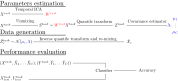
\includegraphics[width=1\textwidth]{figures/condica/method_figure}}
\caption{\textbf{Conditional ICA approach in depth.} 
The approach proceeds by learning a temporal ICA of rest data $X^{rest} \in
\mathbb{R}^{p, n}$ , resulting in
independent sources and unmixing matrix $W^{rest} \in \mathbb{R}^{k, p}$.
%
Applying the unmixing matrix to the task data, we obtain samples in the source
space $S^{task} \in \mathbb{R}^{k, n}$.
%
Afterwards, we map $S^{task}$ to a normal distribution, yielding $Z^{task} \in
\mathbb{R}^{k, n}$. 
%
Then, we estimate the covariance $\Lambda \in \mathbb{R}^{k, k}$ (all classes are assumed to have the
same covariance) and the class-specific means $\boldsymbol{\mu}_1, \dots, \mub_C \in \mathbb{R}^{k}$ according to Ledoit-Wolf's method.
%
For each class $c$, we can draw random samples $\tilde{Z}^{task}_c \in
\mathbb{R}^{k, n_{\mathrm{fakes}}}$ from the
resulting multivariate Gaussian distribution $\mathcal{N}(\mub_c, \Lambda)$ and
obtain fake data $\tilde{X}_c  \in
\mathbb{R}^{p, n_{\mathrm{fakes}}}$
by applying the inverse quantile transform and re-mixing the data using the pseudo inverse of the unmixing matrix.
%
We append these synthetic data to the actual data to create our new augmented
dataset on which we train classifiers.}
\label{Fig11}
\end{figure}
%

\section{Related work}
In image processing, data augmentation is part of standard toolboxes and
typically includes operations like cropping, rotation, translation.
%
On fMRI data these methods do not make much sense as brain condica are not invariant to such transformations.
%
More advanced techniques~\cite{zhuang2019fmri}%\cite{sandfort2019data}
are based on generative models such as GANs or variatonal
auto-encoders~\cite{kingma2013auto}. Although GAN-based method are powerful they are slow and difficult to train~\cite{arjovsky_wasserstein_2017}. In
appendix Table~\ref{app:runningtime:tab}, we show that Conditional ICA is several orders of magnitude faster than GAN-based methods.

Our method is not an adversarial procedure, however it relates to other
powerful generative models such as variatonal
auto-encoders~\cite{kingma2013auto} with which it shares strong similarities.
Indeed the analog of the encoding function in the variational auto-encoder is
given by $e(\xb) = \Lambda^{-\frac12}q(W^{rest} \xb)$ in our model and the analog to the decoding
function in the variational auto-encoder is given by $d(\zb) =
(W^{rest})^{\dagger}q^{-1}(\Lambda^{\frac12}\zb)$ in our model. As in the variational auto-encoder, $e$ approximately maps the distribution of the data to a standardized Gaussian distribution,
while the reconstruction error defined by the difference in l2 norm
$\|d(e(\xb)) - \xb\|^2_2$ must remain small.
Lastly, another classical generative model related to ours is normalizing
flows.  We note that when $W^{rest}$ is squared (no dimension reduction in ICA), the decoding operator $d$ is invertible (its inverse is $e$) making our
model an instance of normalizing flows. 
%
A great property is thus the simplicity and reduced cost of data generation.



\chapter{CondICA in practice}
\label{ch:condica2}
In the previous chapter, we have introduced Conditional ICA, a fast generative
model for task and rest fMRI data.
In this chapter, we first show that the generative model of resting state data shipped in Conditional ICA produces samples that neither linear nor non-linear classifiers are able to distinguish.
% 
Then we benchmark Conditional ICA as a generative model of task data against
various augmentation methods  on their
ability to improve classification accuracy on a large task fMRI dataset.
We find that Conditional ICA yields highest accuracy improvements.
In particular Conditional ICA outperforms GANs and conditional GANs~\cite{mirza2014conditional} while being much easier to optimize and interpret. 
Lastly, we show on 8 different datasets that the use of Conditional ICA results in systematic improvements in classification accuracy ranging from 1\% to 5\%.

\section{Dataset, data augmentation baselines and classifiers used}
\label{sec:condica:datasets}
The unmixing matrices are learned on the rest HCP
dataset~\cite{van2013wu} using 200 subjects.
These data were used after standard
preprocessing, including linear detrending, band-pass filtering
($[0.01, 0.1]Hz$) and standardization of the time courses.
The other 8 datasets~\cite{van2013wu, shafto2014cambridge,
  orfanos2017brainomics, pinel2019functional, pinel2007fast, pinel2013genetic,
  poldrack2016phenome, pinel2013genetic} are obtained from the Neurovault repository~\cite{gorgolewski2015neurovault}.
The classes used in each of these datasets correspond to the activation maps
related to contrasts (such as ``face vs tools'')
present in the set of tasks of each dataset. In table~\ref{fig:dataset:tab}, we
give references to the datasets used as well as the total number of samples
(subjects), the size of train and test sets in each of the cross validation
splits and the number of classes in each dataset. 

\begin{table}
\begin{center}
\begin{tabular}{c|c|c|c}
\hline
Dataset & Subjects, & Train/Test & Neurovault \\
 & classes  &  & collection 
\\ \hline
hcp~\cite{van2013wu}  & 787, 23 & 100/687  &  4337
\\
cam-can \cite{shafto2014cambridge}  & 605, 5 & 100/505  &  4342
\\
brainomics \cite{orfanos2017brainomics}  & 94, 19 & 50/44  &   4341
\\
archi \cite{pinel2019functional}  & 78, 30 & 40/38  &  4339
\\
la5c \cite{poldrack2016phenome}  & 191, 24 & 100/91  &  4343
\\
pinel2012archi \cite{pinel2019functional} & 76, 10 & 40/36  &  1952
\\
pinel2009twins \cite{pinel2013genetic}  & 65, 12 & 35/30  &  1952
\\
pinel2007fast \cite{pinel2007fast} & 133, 10 & 70/63  &  1952
\\\hline\hline
\end{tabular}
\end{center}
\caption{\textbf{Datasets used in the experiments.} The table provides
  references to the datasets that were used for our experiments, with
  the number of subjects, the number of classes, the number of subjects in train
  and test set in each cross validation split and the collection number in Neurovault}
  \label{fig:dataset:tab}
\end{table}


We consider 5 alternative
augmentation methods: \emph{ICA}, \emph{Covariance}, \emph{ICA + Covariance}, \emph{GANs} and \emph{CGANs}.
%
When no augmentation method is applied we use the label \emph{Original}.

The \emph{ICA} covariance method applies ICA to $X^{task}$ to generate unmixing matrices $W^{task}$ and
components $S^{task}=  W^{task} X^{task}$.
%
To generate a sample $\tilde{\xb}_c$ from class $c$, we sample
independently from each component restricted to the samples of class $c$ yielding $\tilde{\sbb}^{task}_c$ and mix the data: $\tilde{\xb}_c = (W^{task})^{\dagger}
\tilde{\sbb}^{task}_c$.
%

The \emph{Covariance} method generates a new sample of
synthetic data in class $c$ by sampling from a Multivariate Gaussian
with mean $\mub_c$ and covariance $\Sigma$, where $\mub_c$ is the
class mean and $\Sigma$ is the covariance of centered task data
estimated using Ledoit-Wolf method.
%
In brief, it assumes normality of the data per class.

The \emph{ICA + Covariance} method combines the augmentation
methods \emph{ICA} and \emph{Covariance}: samples are drawn following
the ICA approach, but with some additive non-isotropic Gaussian noise.
%
As in \emph{ICA} we estimate $W^{task}$ and $S^{task}$ from
$X^{task}$ via ICA.
%
Then we consider $R_{task} = X_{task} - W_{task} S_{task}$ and estimate the
covariance $\Sigma_R$ of $R_{task}$ via LedoitWolf's method.
%
We then generate a data sample $\tilde{\xb}_c$ from class $c$ as with ICA and add
Gaussian noise $\tilde{\nb} \sim \mathcal{N}(0,\Sigma_R)$.
%
Samples are thus generated as $\tilde{\xb}_c + \tilde{\nb}$.

The \emph{GANs} and \emph{CGANs}) methods rely on similar networks. The generator and discriminator have a mirrored architecture with 2 fully connected hidden layer of size (256 and 512).  The number of epochs, batch size, momentum and learning rate are set to 20k, 16, 0.9, 0.01 and we use the Leaky RELU activation function.

We evaluate the performance of augmentation methods through the use of classifiers: logistic regression (LogReg), linear
discriminant analysis with Ledoit-Wold estimate of covariance (LDA) perceptron
with two hidden layers (MLP) and random forrests (RF).
The hyper-parameters in each classifier are optimized through an internal 5-Fold
cross validation. We set the number of iterations in each classifier so that
convergence is reached. The exact specifications are given in table~\ref{fig:classifiers:tab}.

\begin{table}
  \begin{tabular}{ p{.11\textwidth} | p{.3\textwidth} |p{.5\textwidth}}
\hline
  Methods & Optimizer & Hyper-parameters \\
  \hline
LogReg & L-BFGS \newline ($20~000$ iterations) & inverse $L_2$ regularization
strength \newline in $\{0.0001, 0.001, 0.01, 0.1, 1 \}$ \\
  \hline
LDA  & Least-squares solver & Estimation of covariance \newline using Ledoit-Wolf's
                              method \\
  \hline
  RF &  - &  Default parameters in sklearn \\
  \hline
MLP  & Adam \newline ($20~000$ iterations, \newline momentum: $0.9$, \newline
batch size: $32$, \newline learning
       rate: $0.0001$) & $ReLU$ activation function, fully connected
                         architecture with two hidden layers both of size $1024$, L2
                         penalty coefficient: $10^{-5}$
\caption{\textbf{Optimizers and hyper-parameters of classifiers} For each classifier, we give the optimization method used as well as the value of hyper-parameters.}\label{fig:classifiers:tab} 
\end{tabular}
\end{table}


 
\section{Distinguish fake from real HCP resting state data}
This experiment is meant to assess the effectiveness of the data
augmentation scheme in producing good samples.
Data augmentation methods are trained on 200 subjects taken from HCP rest fMRI
dataset which amounts to $960k$ samples (4800
per individual). Then synthetic
data corresponding to $200$ synthetic subjects are produced, yielding
$960k$ fake samples and various classifiers are trained to distinguish fake from
real data using 5-Fold cross validation. The cross-validated accuracy is shown
in table~\ref{tab2}.
Interestingly, we observe a dissociation between linear models (LogReg
and LDA) that fail to discriminate between generated and actual data,
and non-linear models (MLP and RF) that can discriminate samples from
the alternative augmentation methods.
%
By contrast, all classifiers are at chance when Conditional ICA is used.

\begin{table}
\begin{center}
\begin{tabular}{c|cccc}
\hline
Models & LDA  & LogReg & Random Forest &  MLP 
\\ \hline
ICA   & 0.493 & 0.500 & 0.672 &  0.697
\\
Covariance   & 0.473 & 0.461 & 0.610 &  0.626
\\
ICA + Covariance   & 0.509 & 0.495 & 0.685 &  0.706
\\
GANs   & 0.501 & 0.498 & 0.592 &  0.607
\\
CGANs   & 0.498 &  0.493 & 0.579 & 0.604
\\\hline
\textbf{Conditional ICA}  & 0.503 & 0.489 & 0.512 &  0.523
\\\hline\hline
\end{tabular}
\end{center}
  \caption{\textbf{Distinguish fake from real HCP resting state data}
    We use HCP resting state data from $n=200$ subjects ($960k$ samples) and produce an equally
    large amount of fake data ($960k$ samples) using data augmentation methods.
    The table shows the 5-fold cross validated accuracy obtained with various
    classifiers. When Conditional ICA is used, all classifiers are at chance.
    %
    }\label{tab2}
\end{table}
%
\section{Comparing augmentation methods based on classification accuracy on task
  HCP dataset}
In order to compare the different augmentation methods, we measure their 
relative benefit in the context of multi-class classification.
We use 787 subjects from the HCP task dataset that contains 23 classes and
randomly split the dataset into a train set that contains 100 subjects and a test set
that contains 687 subjects. In each split we train augmentation methods on the
train set to generate fake samples corresponding to $200$ subjects.  
These samples are then appended to the train set, resulting in an
augmented train set on which the classifiers are trained. Results, displayed in
table~\ref{condica:tab3}, show that Conditional ICA always yields a higher accuracy
than when no augmentation method is applied. The gains are over 1\% on all
classifiers tested excepts with the random forest classifier which yields much
lower accuracy than other methods.
%
By contrast, ICA+Covariance and ICA lead to a decrease in accuracy
while the Covariance approach leads to non-significant
gains.
%

\begin{table}
  \setlength{\tabcolsep}{0.23em}
  % {\renewcommand{\arraystretch}{1}% for the vertical padding
  \begin{center}
    \begin{tabular}{c|c|c|c | c}
      \hline
      Models & LDA & LogReg & MLP& RF\\
      \hline
      Original           & 0.893 & 0.874 &  0.779 &0.782 \\
    ICA                & 0.814 & 0.840 &  0.803 &0.778\\
    Covariance         & 0.895 & 0.876 &  0.819 &0.780\\
    ICA + Covariance   & 0.816 & 0.840 &  0.815 &0.780\\
    GANs               & 0.877 & 0.863 &  0.771 &0.780\\
    CGANs              & 0.874 & 0.874 &   0.726&0.779 \\
    \hline                                      
      \textbf{Conditional ICA} &  \textbf{0.901} & \textbf{0.890} & \textbf{0.832} &  \textbf{0.783} \\
    \hline\hline
\end{tabular}
\end{center}
\caption{\textbf{Comparing augmentation methods based on classification accuracy on task
      HCP dataset} We compare augmentation methods based on the classification
    accuracy \textbf{(Acc)} obtained by 2 linear classifiers (LDA and LogReg) and two
    non-linear classifier (MLP and RF) trained on augmented datasets on HCP
    Task fMRI data. We report the mean accuracy across 5 splits.}
  \label{condica:tab3}
\end{table}

In table~\ref{app:runningtime:tab}, we give the running-time of GAN based
methods and Conditional ICA. This shows that in contrasts to deep learning based
methods, the computational over-head induced by CondICA is very low.
\begin{table}
  \begin{center}
    \begin{tabular}{|c|c|}
      \hline
      Methods & Running-time (secs)
      \\ \hline
      GANs  & 12948.2 ($\approx$ 3,60 hr)
      \\
      CGANs  & 11015.1 ($\approx$ 3,05 hr)
      \\
      \textbf{Conditional ICA}  & 62 s 
      \\
      \hline
    \end{tabular}
  \end{center}
  \caption{\textbf{Running time.} We display the running time of three methods used
    to generate synthetic data. Conditional ICA is several orders of magnitude faster than
    GANs or CGANs. In practice the computational over-head induced by Conditional ICA is negligible.}\label{app:runningtime:tab}
\end{table}

Lastly, we provide some visualization of fake examples produced by GANs, CGANs and Conditional ICA in figure~\ref{sec:visualization:fig}.
\begin{figure}
  \centerline{\includegraphics[width=0.8\linewidth]{figures/condica/fake_real_viz_v3_redim_improved.png}}
  \caption{\textbf{Data generation visualization.} Visualization of real
    (Original) and synthetic brain maps from three generation methods:
    Conditional ICA, CGANs and GANS. Three cognitive tasks are shown (reward, punish and math).
  }
  \label{sec:visualization:fig}
\end{figure}






\section{Gains in accuracy brought by conditional ICA on eight datasets.}
In this experiment we assess the gains brought by Conditional ICA data
augmentation on the eight different task fMRI datasets refered to in section~\ref{sec:condica:datasets}. The experimental pipeline is exactly the same as with the HCP task dataset.
We report in Fig.~\ref{Fig4} the cross-validated accuracy of
classifiers with and without augmentation.
We notice that the effect of data augmentation is
consistent across datasets, classifiers and splits, with 1\% to 5\% net gains.
%
\begin{figure}
  \centering
  \includegraphics[width=\textwidth]{figures/condica/accuracy_all_datasets_v5.png}
\caption{\textbf{Accuracy of models for eight multi-contrast datasets.} Cross
  validated accuracy of two linear (LDA and LogReg) and one non-linear
  classifier (MLP) with or without using data augmentation.
  %
  The improvement yielded by data augmentation is displayed in red.
  %
  Black error bars indicate standard deviation across splits while white error bars indicate standard deviation across splits with no augmentation.}
\label{Fig4}
\end{figure}
%

Lastly, we provide a sensitivity analysis on the number of components used in
CondICA in figure~\ref{condica:sensitivity:fig}.
CondICA gives good performance for numbers of components between 800 and 1000
components. In all experiments we used $k=900$ components.

\begin{figure}
  \centerline{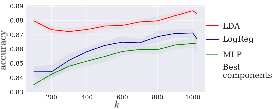
\includegraphics[width=0.8\textwidth]{figures/condica/sensitivity.pdf}}
  \caption{\textbf{Accuracy of augmented discriminative models when
      varying $k$.} We use 100 train subjects from the HCP task dataset to train Conditional ICA with $k$ components and generate $200$ fake subjects.
    Classifiers are trained on the train and fake subjects and tested on the
    left-out 687 subjects. We repeat the procedure
    for various values of $k$ using 5 random splits per value and
    report the mean accuracy across splits as a function of $k$.
    The dotted line represents the number of components that has been
    used in our experiments ($k=900$).
  }
  \label{condica:sensitivity:fig}
\end{figure}






\section{Conclusion}
Conditional ICA produces samples that cannot be distinguished from true actual rest by linear as well as non-linear classifiers, showing that it captures higher-order statistics than naive ICA-based generators.
%
When Conditional ICA is used as a data augmentation method, it yields consistent
improvement in classification accuracy: on 8 tasks fMRI datasets, we observe
increase in accuracy between 1\% and 5\% depending on the dataset and the
classifier used.
Importantly, this performance was obtained without any fine-tuning of
the method, showing its reliability. One can also notice that our experiments cover datasets with different cardinalities, from tens to thousand, and different baseline prediction accuracy.

The systematic performance improvement CanICA yields
makes it a promising candidate for data augmentation in a wide range of
contexts. Future work may focus on its applicability to other decoding tasks
such as the diagnosis of Autism Spectrum Disorder
(ASD)~\cite{eslami2019asd,eslami2019auto,dvornek2017identifying} or
Attention-Deficit/Hyperactivity Disorder detection (ADHD)~\cite{mao2019spatio}. Other extensions of the present work concern the adaptation to
individual feature (e.g. age) prediction where
fMRI has shown some potential.
%

\part{Conclusion}
\chapter{Conclusion}
\section{Resources resulting from this thesis}
\subsection{Mvlearn}
\subsection{Brainiak}
\section{Contributions outside of the scope of the thesis}
\subsection{A deep approach to model complex stimuli}
\subsection{Predicting resting state from fMRI}
\subsection{An optimal transport approach to hyperalignment}
\section{A note about resources used}
All the code is written in Python.
We use Matplotlib for plotting~\cite{hunter2007matplotlib} , scikit-learn for
machine-learning pipelines~\cite{pedregosa2011scikit}, MNE for MEG
processing~\cite{gramfort2013meg}, Nilearn for fMRI processing and for its CanICA implementation~\cite{abraham2014machine}, Brainiak~\cite{kumar2020brainiak} for its SRM implementation. 
% 




\cleardoublepage\include{FrontBackmatter/Bibliography}

\appendix
\part{Appendices}
\chapter{MultiViewICA}
\chapter{MultiViewICA}
\section{Likelihood}
\label{sec:app_likelihood}
\subsection{Initial form of likelihood}\label{sec:appendix:likelihood_transform}

To derive the likelihood, we start by conditioning on $\sbb$. Then, we make a variable transformation from $\xb_i$ to $\nb_i=W_i\xb_i-\sbb$, as opposed to the transformation to $\sbb$ as is usual in ICA. Using the probability transformation formula, we obtain
\begin{equation}
p_{\xb_i|\sbb}(\xb_i|\sbb)=|W_i|p_{\nb_i}(W_i\xb_i-\sbb)    
\end{equation}
where $p_{\nb_i}$ is the density of $\nb_i$. Note that the $\xb_i$ are conditionally independent given $\sbb$, so we have:
\begin{equation}
  p_{\xb|\sbb}(\xb|\sbb)=\prod_{i=1}^m  |W_i| p_{\nb_i}(W_i\xb_i-\sbb)
\end{equation}
and we next get the joint density as:
\begin{equation}
  p_{\xb, \sbb}(\xb,\sbb)=p_{\sbb}(\sbb) \prod_{i=1}^m  |W_i| p_{\nb^i}(W_i\xb_i-\sbb)
\end{equation}
Integrating out $\sbb$ gives Eq.~(\ref{eq:likelihood}).


\subsection{Integrating out the components}\label{sec:appendix:integration}

The integral in question, after factorization, is given by
\begin{equation}
\int_{\sbb} \prod_{j=1}^k \exp \left( -\frac{1}{2\sigma^2} \sum_{i=1}^m ((\wb_j^i)^{\top}\xb_i-s_j)^2 \right) p_{s}(s_j) d\sbb
\end{equation}
which factorizes for each $j$. Denote $y^i_j=(\wb_j^i)^{\top}\xb_i$ and $\tilde{s_j}=\frac1m\sum_{i=1}^m y^i_j$.  Fix $j$, and drop it to simplify notation. Then we need to solve the integral
\begin{align*}
   &\int_s \exp \left(-\frac{1}{2\sigma^2} \sum_{i=1}^m (y^i-s)^2 \right) p_{s}(s)ds\\
   &=\int_s \exp \left(-\frac{1}{2\sigma^2} [ m(\tilde{s}-s)^2 + \sum_{i=1}^m (y^i-\tilde{s})^2] \right) p_{s}(s)ds \\ 
&= \exp \left(-\frac{1}{2\sigma^2}\sum_{i=1}^m (y^i-\tilde{s})^2 \right) 
\int_z \exp \left(-\frac{m}{2\sigma^2} z^2 \right) p_{s}(\tilde{s}-z) dz
\end{align*}

where we have made the change of variable $z=\tilde{s}-s$. The remaining integral simply means that $d$ is smoothed by a Gaussian kernel, which can be computed exactly if $d$ is a Gaussian mixture. We therefore define $f(s) = \log \left(\int_z \exp \left(-\frac{m}{2\sigma^2} z^2 \right) p_{s}(s-z) dz\right)$.
\section{Initialization of MultiViewICA}
\label{sec:app_init}
Since the cost function $\mathcal{L}$ is non-convex, having a good initialization can make a difference in the final result.
% 
We propose a two stage approach.
% 
We begin by applying PermICA on the datasets, which gives us a first set of unimixing matrices $W_1^1, \dots, W_1^m$.
% 
Note that we could also use GroupICA for this task.
% 
Next, we perform a diagonal scaling of the mixing matrices, i.e. we find the diagonal matrices $\Lambda^1, \dots, \Lambda^m$ such that $\mathcal{L}(\Lambda^1W_1^1, \dots, \Lambda^mW_1^m)$ is minimized.
% 
To do so, we employ Algorithm~\ref{algo:mv_ica} but only take into account the diagonal of the descent direction at each step: the update rule becomes $W_i \leftarrow (I_k + \rho \text{Diag}(D))W_i$.
% 
The initial unmixing matrices for Algorithm~\ref{algo:mv_ica} are then taken as $\Lambda^1W_1^1, \dots, \Lambda^mW_1^m$.

Empirically, we find that this two stage procedure allows for the algorithm to start close from a satisfactory solution.
\section{Proofs of Section~\ref{sec:mvica}}
\label{sec:app_proofs}
\subsection{Proof of Prop.~\ref{prop:identifiability}}
\label{app:proof:mvica:identifiability}
We fix a subject $i$. Since $\sbb$ has independent components, so does $\sbb + \nb_i$. Following~\cite{comon1994independent},
Theorem 11, there exists a scale-permutation matrix $P^i$ such that $A'_i =
A_iP^i$. As a consequence, we have $\sbb  + \nb_i = P^i(\sbb' + \nb'^i)$ for all
$i$.

Then, we focus on subject 1 and subject $i \neq 1$:
\begin{align}
  &\sbb + \nb^1 - (\sbb + \nb_i) = P^1(\sbb' + \nb'^1) - P^i(\sbb' + \nb'^i)\\
  &\nb^1 - \nb_i = P^1(\sbb' + \nb'^1) - P^i(\sbb' + \nb'^i)\\
  &\iff P^1\sbb' - P^i\sbb' = P^i \nb'^i - \nb_i + \nb^1 - P^1 \nb'^1 \label{eq:condition_gaussian}
\end{align}
% This shows that $P^1\sbb' - P^i\sbb'$ is Gaussian which can only happen if $P^1= P^i$. 
Since the right hand side of equation (\ref{eq:condition_gaussian}) is a linear combination of Gaussian random variables, this would imply that $P^1\sbb' - P^i\sbb'$ is also Gaussian. However, given that $\sbb'$ is assumed to be non-Gaussian, the equality can only hold if $P^1
= P^i$ and both the right and the left hand side vanish.
Therefore, the matrices $P^i$ are all equal, and there exists a scale and permutation matrix $P$ such that $A'_i = A_iP$.

\subsection{Proof of Prop.~\ref{prop:robust}}
\label{ref:robust}
We consider $W_i = \Lambda (A_i)^{-1}$, where $\Lambda$ is a diagonal matrix.
%
We recall $\xb_i= A_i (\sbb + \nb_i),$ so that $\yb_i = W_i\xb_i= \Lambda(\sbb + \nb_i)$.
%
The gradient of $\loss$ is given by equation~\eqref{eq:gradient}:
\begin{align}
  \mathcal{G}^i &= \frac{1}{m}f'(\tilde{\sbb})(\sbb + \nb_i)^{\top}\Lambda + \frac{1 - 1/m}{\sigma^2} \Lambda\left(\nb_i - \frac{1}{m-1}\sum_{j\neq i} \nb^j\right)(\sbb + \nb_i)^{\top}\Lambda - I_k \\
  & = \frac{1}{m}f'(\Lambda(\sbb + \frac1m\sum_j\nb^j))(\sbb+\nb_i)^{\top} \Lambda + \frac{\sigma'^2(1 - 1/m)}{\sigma^2} \Lambda^2 - I_k
\end{align}
where we write $f'(\sbb) = \begin{bmatrix}f'(s_1) \\ \vdots \\ f'(s_k) \end{bmatrix}$.
Therefore, $\mathcal{G}^i$ is diagonal and constant across subjects (because $f'(\Lambda(\sbb + \frac1m\sum_j\nb^j))(\nb_i)^{\top} = f'(\Lambda(\sbb + \frac1m\sum_j\nb^j))(\nb^{i'})^{\top}$).
Let us therefore consider only its coefficient $(a, a)$, and let $\lambda = \Lambda_{aa}$:
$$
\mathcal{G}^i_{aa} =G(\lambda) = \phi(\lambda)\lambda + \frac{\sigma'^2(1 - 1/m)}{\sigma^2}\lambda^2 - 1,
$$
where $\phi(\lambda) = \frac{1}{m}f'(\lambda(s_a + \frac1m\sum_j n^j_a))(s_a+n_a^i)$. One the one hand, we have $G(0) = -1$. On the other hand, if we assume for instance that $f'$ has sub linear growth (i.e. $|f'(x)| \leq c|x|^{\alpha} +d$ for some $\alpha < 1$) or that $\phi$ is positive, we find that $G(+\infty) = +\infty$.
Therefore, $G$ cancels, which concludes the proof.

\subsection{Stability conditions}
\label{sec:stability}
We consider $W_i = \Lambda (A_i)^{-1}$ where $\Lambda$ is such that the gradients $\mathcal{G}^i$ all cancel. We consider a small relative perturbation of $W_i $ of the form $W_i \leftarrow (I_k + E^i)W_i$, and consider the effect on the gradient.
We define $\Delta^i=\mathcal{G}^i\left((I_k + E^1)W_1, \dots, (I_k + E^m)W_m\right)$.
Denoting $C = \frac{1 - 1/ m}{\sigma^2}$ and $\tilde{\nb} = \frac1m\sum_{i=1}^m \nb_i$, we find:
\begin{align}
     &\Delta^i=\underbrace{\frac1m f'\left(\Lambda(\sbb + \tilde{\nb}) + \frac1m \sum_{j=1}^m E^j\Lambda(\sbb +\nb^j)\right)(\sbb +\nb_i)^{\top}\Lambda(I_k + E^i)^{\top} }_{\Delta_1^i} +\\
     &C\underbrace{\left(\Lambda\nb_i - \frac{1}{m-1}\sum_{j\neq i} \Lambda\nbb^j + E^i\Lambda(\sbb + \nb_i) - \frac{1}{m-1}\sum_{j\neq i} E^j \Lambda(\sbb + \nb^j)\right)(\sbb + \nb_i)^{\top}\Lambda(I_k + E^i)^{\top}}_{\Delta_2^i} \\
     &- I_k\\
\end{align}

The first term is expanded at the first order, denoting $S = \sum_{j=1}^m E^j$:

\begin{align}
    \Delta_1^i &= \frac1m \left(f'(\Lambda(\sbb + \tilde{\nb})) + f''(\Lambda(\sbb + \tilde{\nb}))\odot \left(\frac1m \sum_{j=1}^m E^j\Lambda(\sbb +\nb^j)\right)\right)(\sbb +\nb_i)^{\top}\Lambda(I_k + E^i)^{\top}\\
    &=\frac1m f'(\Lambda(\sbb + \tilde{\nb}))(\sbb + \nb_i)^{\top}\Lambda(I_k + E^i)^{\top} + \frac1{m^2}S\odot  \left(f''(\Lambda(\sbb + \tilde{\nb}))(\sbb^2)^{\top}\Lambda^2 \right)\\
    &+\frac{1}{m^2}E^i\odot\left(f''(\Lambda(\sbb + \tilde{\nb}))((\nb_i)^2)^{\top}\Lambda^2 \right)
\end{align}
The symbol $\odot$ denotes the element-wise multiplication, $f'(\sbb) = \begin{bmatrix}f'(s_1) \\ \vdots \\ f'(s_k) \end{bmatrix}$ and $f''(\sbb) = \begin{bmatrix}f''(s_1) \\ \vdots \\ f''(s_k) \end{bmatrix}$.
Similarly, the second term gives at the first order: 
\begin{align}
    \Delta_2^i &= \sigma'^2\Lambda^2(I_k + E^i)^{\top} + (1 + \sigma'^2)E^i\Lambda^2 - \frac{1}{m-1} (S - E^i) \Lambda^2
\end{align}

Combining this, we find:

\begin{align}
 \Delta^i = (E^i)^{\top} + E^i \odot\Gamma^E
 +S\odot \Gamma^S
\end{align}
where 
$$
\Gamma^E= \left(\frac1{m^2}f''(\Lambda(\sbb + \tilde{\nb}))((\nb_i)^2)^{\top} + (1-\frac1m)\frac{\sigma'^2}{\sigma^2} + \frac{1}{\sigma^2} \right)\Lambda^2
$$
$$
\Gamma^S =\left(\frac1{m^2}f''(\Lambda(\sbb + \tilde{\nb}))(\sbb^2)^{\top} -\frac{1}{m\sigma^2}  \right)\Lambda^2
$$

are $k\times k$ matrices, independent of the subject.
This linear operator is the Hessian block corresponding to the $i$-th subject:
Denoting $\mathcal{H}$ the Hessian, it is the mapping $\mathcal{H}(E^1, \dots, E^m) = (\Delta^1, \dots, \Delta^m)$.

The coefficient $\Delta^i_{ab}$ only depends on $(E^i_{ab}, E^i_{ba}, E^1_{ab},\dots, E^m_{ab})$. Therefore, the Hessian is block diagonal with respect to the blocks of coordinates $(E^1_{ab}, E^1_{ba}, \dots, E^m_{ab}, E^m_{ba})$. Denote $\varepsilon = \Gamma^E_{ab}$, $\varepsilon' = \Gamma^E_{ba}$, $\beta = \Gamma^S_{ab}$ and $\beta'= \Gamma^S_{ba}$. The linear operator for the block is:

$$
K(\varepsilon, \varepsilon', \beta, \beta')=
\left(
    \begin{array}{ll|ll|l|ll}
\varepsilon + \beta & 1       & \beta & 0       & \dots  & \beta & 0       \\
1      & \varepsilon' + \beta' & 0      & \beta' & \dots  & 0      & \beta' \\
\hline
\beta & 0       & \varepsilon + \beta & 1       &        & \beta & 0       \\
0      & \beta' & 1      & \varepsilon' + \beta' & \ddots & 0      & \beta' \\
\hline
\vdots & \vdots  &        & \ddots  & \ddots & \vdots & \vdots  \\
\hline
\beta & 0       & \beta & 0       & \dots  & \varepsilon + \beta & 1       \\
0      & \beta' & 0      & \beta' & \dots  & 1      & \varepsilon' + \beta'
    \end{array}
\right)
$$
The positivity of $\mathcal{H}$ is equivalent to the positivity of this operator for all pairs $a, b$.
We now assume $\beta \beta' > 0$.

First, we should note that $K(\varepsilon, \varepsilon', \beta, \beta') $ is congruent to $K(\varepsilon \sqrt{\frac{\beta'}{\beta}}, \varepsilon' \sqrt{\frac{\beta}{\beta'}}, \sqrt{\beta\beta'}, \sqrt{\beta\beta'})$ via the basis $\text{diag}((\frac{\beta'}{\beta})^{1/4}, (\frac{\beta}{\beta'})^{1/4}, \cdots,(\frac{\beta'}{\beta})^{1/4}, (\frac{\beta}{\beta'})^{1/4})$.
%
We denote to simplify notation $\alpha = \varepsilon \sqrt{\frac{\beta'}{\beta}}$, $\alpha' = \varepsilon' \sqrt{\frac{\beta}{\beta'}}$ and $\gamma = \sqrt{\beta\beta'}$. We only have to study the positivity of $K(\alpha, \alpha', \gamma, \gamma)$.
We have:
$$
K(\alpha, \alpha', \gamma, \gamma) =  I_m  \otimes M_\alpha+ \gamma  \mathbb{1}\otimes I_2, \enspace M_\alpha = 
\begin{pmatrix}
\alpha & 1 \\
1 & \alpha'
\end{pmatrix}
$$
Since $I_m\otimes M_\alpha$ and $\gamma \mathbb{1}\otimes I_2$ commute, the minimum value of $\text{Sp}(K)$ is $\text{min}(I_m\otimes M_\alpha) + \text{min}(\gamma\text{Sp}(\mathbb{1}))=\frac12(\alpha + \alpha' - \sqrt{(\alpha - \alpha')^2 + 4}) + m\min(0, \gamma)$.
Since we assumed $\beta \beta' > 0$ we have $\gamma > 0$. This is similar to the usual ICA case, we find that the condition is $\alpha\alpha' > 1$.

If the following conditions hold for all pair of components $a, b$, the components are a local minimum of the cost function:
\begin{itemize}
    \item $\Gamma^S_{ab}\Gamma^S_{ba}\geq 0$
    \item $\Gamma^E_{ab}\Gamma^E_{ba} > 1$
\end{itemize}
\section{Identifiability for Shared Response Model}
\label{sec:app_identifiability}
The shared response model~\cite{chen2015reduced} (SRM) models the data $\xb_i \in \bbR^v$ of subject $i$ for $i = 1,\dots, m$ as
\begin{align*}
    \xb_i = A_i \sbb + \nb_i \enspace \text{with} \enspace \sbb \sim \Ncal(0, \Sigma), \enspace\nb_i \sim \Ncal(0, \rho_i^2 I_v), \enspace {A_i}^{\top}A_i = I_k
\end{align*}
where $A_i \in \bbR^{v, k}$, $\sbb \in \bbR^p$ and  $\Sigma \in \mathbb{R}^{k, k}$ is a symmetric positive definite matrix.

\begin{proposition}
SRM is not identifiable
\end{proposition}
\begin{proof}
Let us assume the data $\xb_i \enspace i=1, \dots, m$ follow the SRM model with parameters $\Sigma, A_i, \rho_i^2 \enspace i=1, \dots, m$. 

Let us consider an orthogonal matrix $O \in \Ocal_k$.
We call $A'_i = A_i O$ and $\Sigma' = O^{\top} \Sigma O$. 
$\Sigma'$ is trivially symmetric positive definite.

Then the data also follows the SRM model with different parameters $\Sigma', A'_i, \rho_i^2 \enspace i=1, \dots, m$.
\end{proof}

\begin{proposition}
We consider the decorrelated SRM model with an additional decorrelation assumption on the shared responses.
\begin{align*}
\xb_i = A_i \sbb + \nb_i \enspace \text{with} \enspace \sbb \sim \Ncal(0, \Sigma), \enspace\nb_i \sim \Ncal(0, \rho_i^2 I_v), \enspace {A_i}^{\top}A_i = I_k
\end{align*}
where $\Sigma$ is a positive \emph{diagonal} matrix. We further assume that the values in $\Sigma$ are all distinct and ranked in ascending order.
The decorrelated SRM is identifiable up to sign indeterminacies on the columns of 
$\begin{bmatrix}
A_1 \\
\vdots \\
A_m
\end{bmatrix}
$.
\end{proposition}
\begin{proof}
The decorrelated SRM model can be written
\begin{align*}
    &\xb_i \sim \Ncal(0, A_i \Sigma {A_i}^{\top} + \rho_i^2 I_v) \enspace \text{with}\enspace  {A_i}^{\top}A_i = I_k
\end{align*}
where $\Sigma$ is a positive diagonal matrix with distincts values ranked in ascending order.

Let us assume the data $\xb_i \enspace i=1, \dots, m$ follow the decorrelated SRM model with parameters $\Sigma, A_i, {\rho_i}^2 \enspace i=1, \dots, m$. Let us further assume that the data $\xb_i \enspace i=1, \dots, m$ follow the decorrelated SRM model with an other set of parameters $\Sigma', A'_i, {\rho'_i}^2 \enspace i=1, \dots, m$.

Since the model is Gaussian, we look at the covariances.
We have for $i \neq j$
\begin{align*}
    \bbE[\xb_i\left(\xb_j\right)^{\top}] = A_i\Sigma {A^j}^{\top} = A'_i \Sigma'{A'^j}^{\top} \enspace, 
\end{align*}
The singular value decomposition is unique up to sign flips and permutation. Since eigenvalues are positive and ranked the only indeterminacies left are on the eigenvectors. For each eigenvalue a sign flip can occur simultaneously on the corresponding left and right eigenvector.

Therefore we have $\Sigma' = \Sigma$, $A_i = A'_i D^{ij}$ and $A^j = A'^j D^{ij}$ where $D^{ij} \in \bbR^{k, k}$ is a diagonal matrix with values in $\{-1, 1\}$. This analysis holds for every $j \neq i$ and therefore $D^{ij} = D$ is the same for all subjects.

We also have for all $i$
\begin{align*}
    \bbE[\xb_i \left(\xb_i\right)^{\top}] = A_i \Sigma {A_i}^{\top} + \rho_i^2 I_v =  A'_i \Sigma' {A'_i}^{\top}  + {\rho'}_i^2 I_v\\
\end{align*}
We therefore conclude ${\rho'}_i^2 = \rho_i^2, i=1 \dots m$.

Note that if the diagonal subject specific noise covariance $\rho_i^2 I_v$ is replaced by any positive definite matrix, the model still enjoys identifiability.
\end{proof}

\section{fMRI experiments}
\label{sec:app_expts}
\subsection{Dataset description and preprocessing}
\label{preprocessing}
The full brain mask used to select brain regions is available in the Python package associated with the paper.

\paragraph{Sherlock}
In \emph{sherlock} dataset, 17 participants are watching "Sherlock" BBC TV show (beginning of episode 1). 
%
These data are downloaded from \url{http://arks.princeton.edu/ark:/88435/dsp01nz8062179}. 
%
Data were acquired using a 3T scanner with an isotropic spatial resolution of 3 mm. 
%
More information including the preprocessing pipeline is available in~\cite{chen2017shared}.
%
Subject 5 is removed because of missing data leaving us with 16 participants.
%
Although \emph{sherlock} data are downloaded as a temporal concatenation of two runs, we split it manually into 4 runs of 395 timeframes and one run of 396 timeframes so that we can perform 5 fold cross-validation in our experiments.


\paragraph{FORREST}
In FORREST dataset 20 participants are listening to an audio version of the Forrest Gump  movie.
%
FORREST data are downloaded from OpenfMRI~\cite{poldrack2013toward}. 
%
Data were acquired using a 7T scanner with an isotropic spatial resolution of 1~mm (see more details in~\cite{hanke2014high}) and resampled to an isotropic spatial resolution of 3~mm.
%
More information about the forrest project can be found at \url{http://studyforrest.org}.
%
Subject 10 is discarded because not all runs available for other subjects were available for subject 10 at the time of writing.
%
Run 8 is discarded because it is not present in most subjects.
 
\paragraph{RAIDERS}
In RAIDERS dataset, 11 participants are watching the movie "Raiders of the lost ark".
% 
The RAIDERS dataset belongs to the Individual Brain Charting dataset~\cite{ibc}.
% 
Data were acquired using a 3T scanner and resampled to an isotropic spatial resolution of 3~mm.
% 
The RAIDERS dataset reproduces the protocol described in~\cite{haxby2011common}.
%
Preprocessing details are described in~\cite{ibc}.

\paragraph{CLIPS}
In CLIPS dataset, 12 participants are exposed to short video clips. 
%
The CLIPS dataset also belongs to the Individual Brain Charting dataset (\cite{ibc}).
%
Data were acquired using a 3T scanner and resampled to an isotropic spatial resolution of 3~mm.
%
It reproduces the protocol of original studies described in \cite{nishimoto2011reconstructing} and \cite{huth2012continuous}.
%
Preprocessing details are described in~\cite{ibc}.

At the time of writing, the CLIPS and RAIDERS dataset from the individual brain charting dataset \url{https://project.inria.fr/IBC/} are available at \url{https://openneuro.org/datasets/ds002685}.
%
Protocols on the visual stimuli presented are available in a dedicated repository on Github: \url{https://github.com/hbp-brain-charting/public_protocols}.
% The informed consent of all subjects was obtained before scanning.
% Bertrand: There is no reason you deal with that

\subsection{Reconstructing the BOLD signal of missing subjects: Discussion on ROIs choice}
\label{brainmaps}

The quality of the reconstructed BOLD signal varies depending on the choice of the region of interest. In Figure~\ref{fig:brainmaps}, we plot for GroupICA, SRM and MultiViewICA, the R2 score per voxel using 50 components for datasets \emph{sherlock}, \emph{forrest}, \emph{raiders} and \emph{clips}. As could be anticipated from the task definition, \emph{forrest} obtains high reconstruction accuracy in the auditory cortices, while \emph{clips} shows good reconstruction in the visual cortex (occipital lobe mostly); the richer \emph{sherlock} and \emph{raiders} datasets yield good reconstructions in both domains, but also in other systems (language, motor).
%
We also see visually see that data reconstructed by MultiViewICA are
a better approximation of the original data than other methods.
%
This is particularly obvious for the \emph{clips} datasets where it is
clear that voxels in the posterior part of the superior
temporal sulcus are better recovered by MultiViewICA than by SRM or
GroupICA.

In order to determine the ROIs, we focus on the R2 score per voxel between the BOLD signal reconstructed by GroupICA and the actual bold signal. We run GroupICA with $10, 20$ and $50$ components and select the voxels that obtained a positive R2 score for all sets of components.
%
We discard voxels with an R2 score above 80\% as they visually correspond to artefacts and apply a binary opening using a unit cube as the structuring element. The chosen regions are plotted in figure~\ref{fig:roi}.

\begin{figure}
  \centering
  \includegraphics[width=\textwidth]{figures/mvica/reconstruction_score_fullbrain.pdf}
  \caption{\textbf{Reconstructing the BOLD signal of missing subjects: Reconstruction R2 score per voxel} We plot for GroupICA, SRM and MultiViewICA, the R2 score per voxel using 50 components for datasets \emph{sherlock}, \emph{forrest}, \emph{raiders} and \emph{clips}. We visually see that data reconstructed by MultiViewICA are more faithful reproduction of the original data than other methods.}
  \label{fig:brainmaps}
\end{figure}

\begin{figure}
  \centering
  \includegraphics[width=\textwidth]{figures/mvica/reconstruction_score_roi.pdf}
  \caption{\textbf{Data-driven choice of ROI} Chosen ROIs for the experiment: Reconstructing the BOLD signal of missing subjects.}
  \label{fig:roi}
\end{figure}

\subsection{Between-runs time-segment matching}
\label{app_spatialmaps}

\begin{figure}
  \centering
  \includegraphics[width=\textwidth]{figures/mvica/swetha_exp_full_fit.pdf}
  \caption{\textbf{Between runs time-segment matching}. Interesting components correlates more when they correspond to the same stimulus (same scenes of the movie) than when they correspond to distinct stimuli (different scenes).
  %We show that when MultiView ICA is used, we can locate a target time-segment in one session using the data of another session corresponding to the same stimuli.
  We extract 20 components and report the mean accuracy of the 3 best performing components}
  \label{fig:swetha}
\end{figure}

We measure the ability of each algorithm to extract meaningful shared components that correlate more when they correspond to the same stimulus than when they correspond to distinct stimuli. We use the \emph{raiders-full} dataset, which allows this kind of analysis because subjects watch some selected scenes from the movie twice, during the first two runs (1 and 2) and the last two (11 and 12).
%
First, the forward operators are learned by fitting each algorithm with 20 components on the data of all 11 subjects using all 12 runs. We then select a subset of 8 subjects and the shared components are computed by applying the forward operators and averaging.
%
We select a large target time-segment ($50$
timeframes) taken at random from run 1 and 2, and we try to localize the corresponding sample time-segment from the 10 last runs using a single component of the shared components.
%
The time-segment is said to be
correctly classified if the correlation between the target and corresponding sample
time-segment is higher than with any other time-segment (partially overlapping windows are excluded).
%
In contrast to the \emph{between subject time-segment matching} experiment, we obtain one accuracy score per component.
%
We repeat the experiment 10 times with different subsets of subjects randomly chosen and report the mean accuracy of the 3 best performing components in Figure~\ref{fig:swetha}. Error bars correspond to a 95~\% confidence interval.
%
MultiView ICA achieves the highest accuracy.

We then focus on the 3 best performing components of MultiView ICA. For each component, we plot in Figure~\ref{fig:app_spatialmaps} (left) the shared components during two sets of runs where subjects were exposed to the same scenes of the movie. We then study the localisation of these components.
%
We average the forward operators across subjects and plot the columns corresponding to the components of interest in Figure~\ref{fig:app_spatialmaps} (right).
%
As each column is seen as a set of weights over all voxels, it represents a spatial map.

The component 1 of the shared responses follows almost the same pattern in the two set of runs corresponding to the same scenes of the movie. The spatial map corresponding to component 1 highlights the language network.
%
In component 2, the temporal patterns during the viewing of identical scenes are also very similar. The corresponding spatial map highlights the visual network especially the visual dorsal pathway.
%
In component 3, there exists a similarity however less striking than with the two previous components. The corresponding spatial map highlights a contrast between the spatial attention network and the auditory network.

\begin{figure}
  \centering
  \includegraphics[width=\textwidth]{figures/mvica/swetha_exp_full_fit_appendix.pdf}
  \caption{\textbf{Between-runs time segment matching: spatial maps and timecourses} \emph{Left:} Timecourses of the 3 shared components yielding the highest accuracy. The two displayed set of runs correspond to the same scenes in the movie. \emph{Right:} Localisation of the same shared components in the brain}
  \label{fig:app_spatialmaps}
\end{figure}

\subsection{Reproducing time-segment matching experiment}
\label{appendix_reproduce}
We reproduce the time-segment matching experiments described in \cite{chen2016convolutional} and \cite{zhang2016searchlight} and use two fold classification over runs instead of 5-fold as we have done in the main paper. We used the sherlock data available at \url{http://arks.princeton.edu/ark:/88435/dsp01nz8062179} and the full brain mask provided in the Python package associated with the paper. We applied high-pass filtering (140 s cutoff) and the time series of each voxel were normalized to zero mean and unit variance.

The results are available in Figure~\ref{fig:supp_timesegment}.

\begin{figure}
  \centering
  \includegraphics[width=0.6\textwidth]{figures/mvica/timesegment_matching_cae.pdf}
  \caption{\textbf{Reproducing the time-segment matching experiment of \cite{chen2016convolutional}~\cite{zhang2016searchlight}} Mean classification accuracy - error bars represent 95\% confidence interval}
  \label{fig:supp_timesegment}
\end{figure}

\subsection{Impact of the hyperparameter $\sigma$ }
\label{sec:app_sigma_impact}
On top of the theoretical guarantees about the robustness of our method to the choice of the $\sigma$ parameter, we investigate its practical impact on the time-matching segment experiment, on the Sherlock dataset with $10$ components.
%
We compute the accuracy of the multi-view ICA pipeline with different choice of $\sigma$.
%
This is reported in Fig.~\ref{fig:supp_noise_sensitivity}. 
%
The accuracy is constant for a wide range of $\sigma$, only decreasing when $\sigma$ attains very high values.
\begin{figure}
  \centering
  \includegraphics[width=0.6\textwidth]{figures/mvica/noise_sensitivity_reb.pdf}
  \caption{\textbf{Effect of the parameter $\sigma$}: We compute the accuracy of the multiview-ICA pipeline on the time-segment matching experiment for various values of the $\sigma$ hyperparameter over a grid. The accuracy varies only marginally with $\sigma$.}
  \label{fig:supp_noise_sensitivity}
\end{figure}

\section{Related Work}
\label{sec:app_rel_work}
The following table describes some usual method for extracting shared components from multiple subjects datasets.
The column "Modality/Components" describes the type of data for which each algorithm was \emph{initially} proposed, even though each algorithm could be applied on any type of data. 
%
The components type can be either temporal if extracted components are time courses or spatial if they are spatial patterns. 
%
\begin{center}
\begin{longtable}{ |p{.15\textwidth} | p{.2\textwidth} |p{.2\textwidth}| p{.3\textwidth}|}
\hline
\textbf{Method} & \textbf{Modality/Components} &\textbf{Dimension reduction} & \textbf{Description}  \\
\hline
SRM \cite{chen2015reduced} & 
fMRI/Temporal
&
SRM
&
The model is $\xb_i = A_i\sbb + \nb_i$, with \emph{Gaussian} components and \emph{orthogonal} mixing matrices $A_i$\\
\hline
GroupPCA~\cite{smith2014group} &
fMRI/Spatial
&
GroupPCA
&
A memory efficient implementation of PCA applied on temporally concatenated data.\\
\hline
GIFT~ \cite{calhoun2001method} & 
fMRI/Spatial
&
Individual PCA + Group PCA (on component-wise concatenated data)
&
Single-subject ICA is applied on the aggregated data\\
\hline
EEGIFT~ \cite{eichele2011eegift} & 
EEG/Temporal
&
Individual PCA + Group PCA (on component-wise concatenated data)
&
Single-subject ICA is applied on the aggregated data\\
\hline
PermICA &
Any
&
Any
&
Single-subject ICA is applied on each subject's data, and the components are matched using the Hungarian algorithm\\
\hline
Clustering approach~\cite{esposito2005independent}&
fMRI/Spatial
&
Individual PCA
&
Single-subject ICA is applied on each subject's data, and the components are matched using a hierarchical clustering algorithm.\\
\hline
Measure projection analysis~\cite{bigdely2013measure}&
EEG/Temporal
&
Individual PCA
&
Single-subject ICA is applied on each subject's data, and the components are matched using a hierarchical clustering algorithm.\\
\hline
TensorICA \cite{beckmann2005tensorial} &
fMRI/Spatial
&
Group PCA (on spatially concatenated data)
&
TensorICA incorporates ICA assumptions into the PARAFAC model. The mixing matrices $A_1 \cdots A_n$ are such that $A_i = A D_i$ where $A$ is common to all subjects and $D_i$ are subject specific diagonal matrices.\\  
\hline
Unifying Approach of \cite{guo2008unified} &
fMRI/Spatial
&
Group PCA (on spatially concatenated data) + GroupPCA (on component-wise concatenated data).
&
The model is $\xb_i = A_i\sbb + \nb_i$ with a Gaussian mixture model on independent components and a matrix normal prior on the noise. \\
\hline
SR-ICA \cite{zhang2016searchlight} &
fMRI/Temporal
&
SR-ICA
&
SR-ICA incorporates ICA assumptions into the shared response model.  \\
\hline
CAE-SRM \cite{chen2016convolutional}
&
fMRI/Temporal
&
CAE-SRM
&
A convolutional auto-encoder is used to perform the unmixing. \\  
\hline
CanICA \cite{varoquaux2009canica} &
fMRI/Spatial
&
Individual PCA + multi set CCA (on component-wise concatenated data)
&
CanICA applies single-subject ICA on data reduced with PCA and CCA.
 \\  
\hline
Spatial ConcatICA~\cite{svensen2002ica} &
fMRI/Spatial
&
Group PCA (on spatially concatenated data)
&
ICA is applied on spatially concatenated data. The mixing is constrained to be the same across all subjects.
 \\  
 \hline
Temporal ConcatICA~\cite{cong2013validating} &
EEG/Temporal
&
Group PCA (on temporally concatenated data)
&
ICA is applied on temporaly concatenated data. The mixing is constrained to be the same across all subjects.
 \\  
\hline
coroICA \cite{pfister2019robustifying} &
Any
&
Any
&
The model is  $\xb_i = A\sbb_i + \nb_i$. The mixing is constrained to be the same across all subjects. \\
%\hline
%Arbitrary correlation factor analysis of~\cite{Monti18UAI} &
%fMRI/Temporal &
%Any &
%The probabilistic model of~\cite{Monti18UAI} assumes the mixing matrix is orthogonal, positive and shared across subjects but not necessarily square. It learns subjects specific co-variance matrices.  \\
\hline
\end{longtable}
\end{center}
\vspace{-10mm}
An additional related model is described in~\cite{gresele2019incomplete}. Similarly to our work, the ICA model has noise on the components side. However, the model involves nonlinear mixings, which are computationally unfeasible to optimize via maximum likelihood; a contrastive learning scheme is therefore adopted, and the likelihood is not derived in closed form. No evaluation on neuroimaging datasets is presented.

\section{Detailed Cam-CAN components}
\label{sec:app_montages}
We display each of the 11 shared components found by Multiview ICA on the Cam-CAN. The time-courses are on the left, the corresponding brain maps are on the right.


{\centering
\includegraphics[width=0.3\textwidth]{figures/mvica/camcan_source_0.pdf}%
\raisebox{0.2\height}{\includegraphics[width=0.68\textwidth]{figures/mvica/montage_0.png}} \\
\includegraphics[width=0.3\textwidth]{figures/mvica/camcan_source_1.pdf}%
\raisebox{0.2\height}{\includegraphics[width=0.68\textwidth]{figures/mvica/montage_1.png}} \\
\includegraphics[width=0.3\textwidth]{figures/mvica/camcan_source_2.pdf}%                        
\raisebox{0.2\height}{\includegraphics[width=0.68\textwidth]{figures/mvica/montage_2.png}} \\
\includegraphics[width=0.3\textwidth]{figures/mvica/camcan_source_3.pdf}%  
\raisebox{0.2\height}{\includegraphics[width=0.68\textwidth]{figures/mvica/montage_3.png}} \\
\includegraphics[width=0.3\textwidth]{figures/mvica/camcan_source_4.pdf}%
\raisebox{0.2\height}{\includegraphics[width=0.68\textwidth]{figures/mvica/montage_4.png}} \\
\includegraphics[width=0.3\textwidth]{figures/mvica/camcan_source_5.pdf}%
\raisebox{0.2\height}{\includegraphics[width=0.68\textwidth]{figures/mvica/montage_5.png}} \\
\includegraphics[width=0.3\textwidth]{figures/mvica/camcan_source_6.pdf}%
\raisebox{0.2\height}{\includegraphics[width=0.68\textwidth]{figures/mvica/montage_6.png}} \\
\includegraphics[width=0.3\textwidth]{figures/mvica/camcan_source_7.pdf}%
\raisebox{0.2\height}{\includegraphics[width=0.68\textwidth]{figures/mvica/montage_7.png}} \\
\includegraphics[width=0.3\textwidth]{figures/mvica/camcan_source_8.pdf}%
\raisebox{0.2\height}{\includegraphics[width=0.68\textwidth]{figures/mvica/montage_8.png}} \\
\includegraphics[width=0.3\textwidth]{figures/mvica/camcan_source_9.pdf}%
\raisebox{0.2\height}{\includegraphics[width=0.68\textwidth]{figures/mvica/montage_9.png}} \\
\includegraphics[width=0.3\textwidth]{figures/mvica/camcan_source_10.pdf}%
\raisebox{0.2\height}{\includegraphics[width=0.68\textwidth]{figures/mvica/montage_10.png}} \\
}

\section{Average forward operators on fMRI datasets}
\label{sec:spatial_maps}
We display the average forward operator across subjects on the Raiders, Forrest, Clips and Sherlock datasets obtained with MultiViewICA and GroupICA with 5 components. A 5~mm spatial smoothing was applied on all datasets, and the confound signals corresponding to the 5 components with the highest variance were removed before applying MultiViewICA or GroupICA.

{\centering

  \includegraphics[width=\textwidth]{figures/mvica/maps_forrest.png} \\
  \includegraphics[width=\textwidth]{figures/mvica/maps_sherlock.png} \\
  \includegraphics[width=\textwidth]{figures/mvica/maps_gallant.png} \\
  \includegraphics[width=\textwidth]{figures/mvica/maps_raiders.png} \\
}

\section{Synthetic benchmark using additive noise on the sensors}
\label{app:complex_cov}
We generate data according to the model $\xb_i = A_i\sbb + \nb_i$, where $\xb_i \in \mathbb{R}^{50}$, $\sbb \in \mathbb{R}^{20}$, and $\nb_i\sim \mathcal{N}(0, \sigma^2 I_{50})$. After applying individual PCA to obtain signals of dimension $20$, we apply the different ICA algorithms and report the reconstruction error in fig.~\ref{fig:reconstruction_synth}.

\begin{figure}
  \center
  \includegraphics[width=0.5\linewidth]{figures/mvica/distance.pdf}
  \caption{Synthetic experiment with model $\xb_i = A_i\sbb^i + \nb_i$} %{Light Unit}
  \label{fig:reconstruction_synth}
\end{figure}

\section{Summary of our quantitative results}
\label{sec:app_real_data}
Our quantitative results for the fMRI experiments of time-segment matching and BOLD signal reconstruction and on for the MEG phantom data experiment are summarized, respectively, in Table~\ref{tab:timeseg}, Table~\ref{tab:recon} and Table~\ref{tab:meg}. All methods are compared upon extraction of components with the same dimensionality ($20$ components).

\begin{table}
    \centering
    \begin{tabular}{|c|c | c | c|}
            \hline
         \textbf{Dataset} & \textbf{Method} & \textbf{Accuracy} & \textbf{Confidence interval} \\
         \hline
clips   & Chance      & 0.002&[0.001, 0.003] \\
        & CanICA    & 0.130&[0.112, 0.147] \\
        & PCA + GroupICA      & 0.124&[0.109, 0.139] \\
        & GroupICA    & 0.152&[0.133, 0.171] \\

        & PermICA     & 0.147&[0.126, 0.169] \\
        & SRM         & 0.115&[0.104, 0.126] \\
        & MultiViewICA& \textbf{0.167}&[0.142, 0.192] \\
        \hline
forrest & Chance      & 0.002&[0.001, 0.002] \\
        & CanICA    & 0.192&[0.170, 0.214] \\
        & PCA + GroupICA      & 0.088&[0.077, 0.098] \\
        & GroupICA    & 0.154&[0.137, 0.170] \\
        & PermICA     & 0.135&[0.118, 0.152] \\
        & SRM         & 0.188&[0.173, 0.203] \\
        & MultiViewICA& \textbf{0.448}&[0.411, 0.484] \\
        \hline
raiders & Chance      & 0.002&[0.001, 0.003] \\
        & CanICA    & 0.256&[0.220, 0.291] \\
        & PCA + GroupICA      & 0.331&[0.289, 0.372] \\
        & GroupICA    & 0.321&[0.281, 0.361] \\
        & PermICA     & 0.381&[0.341, 0.421] \\
        & SRM         & 0.265&[0.240, 0.289] \\
         & MultiViewICA& \textbf{0.408}&[0.358, 0.458] \\
         \hline
sherlock& Chance      & 0.005&[0.003, 0.006] \\
        & CanICA    & 0.607&[0.567, 0.648] \\
        & PCA + GroupICA      & 0.454&[0.416, 0.492] \\
        & GroupICA    & 0.519&[0.481, 0.556] \\
        & PermICA     & 0.399&[0.365, 0.434] \\
        & SRM         & 0.493&[0.465, 0.520] \\
        & MultiViewICA& \textbf{0.873}&[0.844, 0.903] \\
\hline
    \end{tabular}
    \caption{Timesegment matching: Summary of our quantitative results. We report the mean accuracy across cross-validation splits.}
    \label{tab:timeseg}
\end{table}

\begin{table}
    \centering
    \begin{tabular}{|c|c | c | c|}
            \hline
         \textbf{Dataset} & \textbf{Method} & \textbf{R2 score} & \textbf{Confidence interval} \\
         \hline
         clips   & Chance              & 0.000&[0.000 ,0.000] \\
        & CanICA            &  0.110&[ 0.097 , 0.123] \\
        & PCA + GroupICA              &  0.075&[ 0.058 , 0.092] \\
        & GroupICA            &  0.077&[ 0.059 , 0.094] \\
        & PermICA             &  0.099&[ 0.087 , 0.111] \\
        & SRM                 &  0.081&[ 0.069 , 0.094] \\
        & MultiViewICA        &  \textbf{0.114}&[ 0.099 , 0.128] \\
        \hline
forrest & Chance              & 0.000&[0.000 ,0.000] \\
        & CanICA            &  0.181&[ 0.169 , 0.193] \\
        & PCA + GroupICA              &  0.072&[ 0.054 , 0.090] \\
        & GroupICA            &  0.081&[ 0.062 , 0.099] \\
        & PermICA             &  0.098&[ 0.090 , 0.106] \\
        & SRM                 &  0.180&[ 0.168 , 0.193] \\
        & MultiViewICA        &  \textbf{0.191}&[ 0.177 , 0.204] \\
        \hline
raiders & Chance              & 0.000&[0.000 ,0.000] \\
        & CanICA            &  0.136&[ 0.122 , 0.149] \\
        & PCA + GroupICA              &  0.063&[ 0.045 , 0.080] \\
        & GroupICA            &  0.062&[ 0.043 , 0.081] \\
        & PermICA             &  0.107&[ 0.091 , 0.124] \\
        & SRM                 &  0.138&[ 0.121 , 0.154] \\
        & MultiViewICA        &  \textbf{0.144}&[ 0.124 , 0.164] \\
        \hline
sherlock& Chance              & 0.000&[0.000 ,0.000] \\
        & CanICA            &  0.156&[ 0.141 , 0.172] \\
        & PCA + GroupICA              &  0.087&[ 0.065 , 0.108] \\
        & GroupICA            &  0.091&[ 0.070 , 0.112] \\
        & PermICA             &  0.067&[ 0.055 , 0.078] \\
        & SRM                 &  \textbf{0.164}&[ 0.147 , 0.181] \\
        & MultiViewICA        &  0.161&[ 0.142 , 0.180] \\
        \hline

         
    \end{tabular}
    \caption{Reconstructing the BOLD signal of missing subjects: Summary of our quantitative results. We report the mean R2 score across cross-validation splits.}
    \label{tab:recon}
\end{table}

\begin{table}
    \centering
    \begin{tabular}{|c|c|c|c}
    \hline
         \textbf{Method} & \textbf{Reconstruction error} & \textbf{1st and 3d quartiles} 
         \\
         \hline
         MultiViewICA & \textbf{0.0045} & [0.0039, 0.0052] \\ 
GroupICA & 0.1098 & [0.0549, 0.1734] \\ 
PCA+GroupICA & 0.1111 & [0.0760, 0.1502] \\ 
PermICA & 0.0730 & [0.0423, 0.1037] \\ 
\hline
    \end{tabular}
    \caption{Phantom MEG data: Summary of our quantitative results with 2 epochs. We report the median reconstruction error across cross-validation splits.}
    \label{tab:meg}
\end{table}


\chapter{ShICA}
\section{Lemmas}
\label{app:sec:lemmas}
\begin{lemma}
\label{lemma:ica}
Let $\sbb \in \mathbb{R}^k$ and $\sbb'\in \mathbb{R}^k$ have independent components among which $g$ are Gaussian, and $P$ a rotation matrix such that $\sbb = P\sbb'$. Then, $P=\Pi^{-1} O \Pi'$ where $\Pi$ and $\Pi'$ are sign and permutation matrices such that the first $g$ components of $\Pi \sbb$ and $\Pi' \sbb'$ are Gaussian and $O$ is a block diagonal matrix such that $O^{(g)}$, the first $g \times g$ block of $O$, is orthogonal and the other block is identity.
\end{lemma}
\begin{proof}
  From~\cite{comon1994independent}, Theorem 10:
  Assume $\sbb = P\sbb'$, if the column $j$ of $P$ has more than one non-zero element then $s'_j$ is Gaussian. 
  
  Let us define permutations $\Pi_1$, $\Pi'_1$ such that the first $g$ components of $\Pi_1 \sbb$ and $\Pi'_1 \sbb'$ are Gaussian and $P_1  = \Pi_1 P (\Pi'_1)^{-1}$. We can see that $P_1$ is orthogonal.
  
  We have $\Pi_1 \sbb = P_1 \Pi'_1 \sbb'$. So the last $p-g$ columns of $P_1$ contain at most one non-zero element. Using orthogonality of $P_1$ this non-zero element has value $1$ or $-1$ and is also the only one in its line. Let us focus on column $l > g$. Assume column $l$ has its non-zero element at index $k \leq g$. Then line $k$ in $P_1$ is only non-zero at index $l$ and therefore $(\Pi_1 \sbb)_k$ (which is Gaussian) is equal to $(\Pi'_1 \sbb')_l$ (which is not). Therefore column $l$ can only have its non-zero element at an index greater than $g$. This shows that $P_1$ is block diagonal $P_1 = \begin{bmatrix} O_g & 0 \\ 0 & P_2 \end{bmatrix}$ where $O_g$ is orthogonal  and $P_2$ is a sign and permutation matrix.
  \begin{align}
      &\begin{bmatrix} O_g & 0 \\ 0 & P_2 \end{bmatrix} = \Pi_1 P (\Pi'_1)^{-1} \\
      & \iff \begin{bmatrix} O_g & 0 \\ 0 & I \end{bmatrix} \begin{bmatrix} I & 0 \\ 0 & P_2 \end{bmatrix}  = \Pi_1 P (\Pi'_1)^{-1} \\
      & \iff \Pi_1^{-1} \begin{bmatrix} O_g & 0 \\ 0 & I \end{bmatrix} \begin{bmatrix} I & 0 \\ 0 & P_2 \end{bmatrix} \Pi'_1  = P
  \end{align}
  
  Therefore setting $\Pi' =   \begin{bmatrix} I & 0 \\ 0 & P_2 \end{bmatrix} \Pi'_1$ and $\Pi = \Pi_1$ and $O= \begin{bmatrix}O_g & 0 \\ 0 & I  \end{bmatrix}$ concludes the proof.
  
\end{proof}

\begin{lemma}
\label{lemma:eigdecomp}
Assume that Assumption 2 holds for $\Sigma_i$, and that there is an orthogonal matrix $P$ and diagonal matrices $\Sigma_i'$ such that for all $i$, $\Sigma_i' = P\Sigma_iP^{\top}$. Then, $P$ is a permutation matrix.
\end{lemma}
\begin{proof}
The proof is in two parts. First, we show that there exist some coefficients $\alpha_1, \dots, \alpha_m$ such that the matrix $\sum_i\alpha_i\Sigma_i$ has distinct coefficients on the diagonal. Then, since we have $\sum_i\alpha_i\Sigma'_i = P\left(\sum_i\alpha_i\Sigma_i\right)P^{\top}$, and the diagonal $\sum_i\alpha_i\Sigma_i$ has distinct entries, we can invoke the unicity of the eigenvalue decomposition for symmetric matrices, which shows that $P$ is necessarily a permutation matrix.
Now, the only thing left is to prove is that Assumption 2 implies the existence of this linear combination.

We assume by contradiction that any linear combination of the $\Sigma_i$ has two equal entries.

For $\alpha = [\alpha_1, \dots, \alpha_m]$, we let $\mathcal{S}(\alpha) = \diag(\sum_i\alpha_i\Sigma_i)\in\bbR^p$, where $\diag(\cdot)$ extracts the diagonal entries. The operator $\mathcal{S}$ is linear.
%
We now define for $j, j'\leq p$ the linear form $\ell_{jj'}(\alpha) = \mathcal{S}(\alpha)_j - \mathcal{S}(\alpha)_{j'}\in\bbR$. The assumption on the linear combinations of $\Sigma_i$ simply rewrites:
For all $\alpha\in\bbR^m$, there exists $j, j'\leq p$ such that $\ell_{jj'}(\alpha) = 0$.

From a set point of view, this relationship writes
$$
\bigcup_{j, j'}\mathrm{Ker}(\ell_{jj'}) = \bbR^m\enspace.
$$
Since the $\ell_{jj'}$ are all linear forms, the $\mathrm{Ker}(\ell_{jj'})$ are subspaces of dimensions $m$ or $m-1$, and since their union is of dimension $m$, there exists $j, j'$ such that  $\mathrm{Ker}(\ell_{jj'}) = \bbR^m$, i.e. such that $\ell_{jj'} = 0$.

As a consequence, we have for all $\alpha$, $\mathcal{S}(\alpha)_j = \mathcal{S}(\alpha)_{j'}$. This implies that the sequences $(\Sigma_{ij})_i$ and $(\Sigma_{ij'})_i$ are equal, which contradicts Assumption 2.


We have therefore shown that Assumption 2 implies the existence of a linear combination of the $\Sigma_i$ that has distinct entries, which concludes the proof.
\end{proof}


\begin{lemma}
\label{lemma:nonzerocoord}
Let us consider the following eigenvalue problem:
 \begin{align}
  & \begin{bmatrix} I + \Sigma_1 & I & \dots & I \\
    I & I + \Sigma_2 & \ddots & \vdots \\
    \vdots &  \ddots & \ddots & I  \\
    I & \dots & I  &I + \Sigma_m
  \end{bmatrix} \zb = \lambda \begin{bmatrix}
    I + \Sigma_1 & 0 & \dots  & 0 \\
    0 & I + \Sigma_2 & \ddots & \vdots \\
    \vdots & \ddots & \ddots & 0 \\
    0& \dots  & 0 &  I + \Sigma_m  \\
  \end{bmatrix} \zb
  \label{reducedeig}
\end{align}
where $\forall i, \enspace 1 \leq i \leq m, \enspace  \Sigma_m \in \bbR^{p, p}$ are positive diagonal matrices and I is the identity matrix.
If the first $p$ eigenvalues are distincts, the first $p$ eigenvectors $\zb^1, \dots, \zb^p, \zb^i \in \mathbb{R}^{mp}$ have different first non-zero coordinates.
\end{lemma}
%\bt{You implicitly assume that D is the block-diagonal part of C ?}
\begin{proof}
We sort the eigenvectors in $p$ groups of $m$ vectors so that all
vectors in group $l$ have their $l$-th coordinate
different from 0.
Let $\zb^{(l)}$ be an eigenvector in group $l$ and let us call $\wb_l \in
\mathbb{R}^{m}$ the non-zero coordinates of this eigenvector: $\forall i \in \{1 \dots m \}, w_{li} = z^{(l)}_{l + (i-1)p}$.

We have:
\begin{align}
\begin{bmatrix}
  1 + \Sigma_{1l} & 1 & \dots & 1  \\
  1 & 1 + \Sigma_{2l} & \ddots  &\vdots \\
  \vdots & \ddots & \ddots & 1  \\
  1 & \dots & 1 & 1 + \Sigma_{ml}  \\
\end{bmatrix} \wb_l =  \begin{bmatrix}
  1 + \Sigma_{1l} & 0 & \dots  & 0 \\
  0 & 1 + \Sigma_{2l} & \ddots & \vdots \\
  \vdots & \ddots & \ddots & 0 \\
  0& \dots  & 0 &  1 + \Sigma_{ml}  \\
\end{bmatrix} \wb_l \lambda_l
\label{eigsimp}
\end{align}

We now show that the biggest eigenvalue of~\eqref{eigsimp} is strictly above 1 while all
others are strictly below 1. The core of the proof comes from the study of the eigenvalues of a matrix modified by a rank 1 matrix. The reasoning we use here follows~\cite{golub1973some} (end of section 5).

Let us introduce 
$K^l = \diag(\Sigma_{1l} \dots \Sigma_{ml})$ and $\ub = \begin{bmatrix} 1 \\ \vdots \\ 1 \end{bmatrix}$.
Let us drop the index $l$ in the notations for simplicity.

The problem can be rewritten
\begin{align}
  &(\ub \ub^{\top} + K) \wb =  (I + K) \wb \lambda \\
  & \iff (I + K)^{-1}(\ub \ub^{\top} + K) \wb =   \wb \lambda
\end{align}

The characteristic polynomial is given by:
\begin{align}
  &\mathcal{P}(\lambda) = \det( (I + K)^{-1} K - \lambda I + (I + K)^{-1} \ub \ub^{\top}) \label{carpol} \\
  &\propto \det( I + ((I + K)^{-1} K - \lambda I)^{-1}(I + K)^{-1} \ub \ub^{\top})
\end{align}
where we implicitly focus here on eigenvalues $\lambda$ such that $\det((I + K)^{-1} K - \lambda I) \neq 0 \iff \forall i, \lambda \neq \frac{k_i}{1 + k_i}$.

We then use the following property:
Let $A \in \mathbb{R}^{a, b}$ and $B \in \mathbb{R}^{b, a}$ we have
$\det(I_a + AB) = \det(I_b + BA)$.

Let us call $\chi(\lambda) = \det( I + ((I + K)^{-1} K - \lambda I)^{-1}(I + K)^{-1} \ub \ub^{\top})$ we have:
\begin{align}
\chi(\lambda)
  &= 1 + \ub^{\top}((I + K)^{-1} K - \lambda I)^{-1}(I + K)^{-1} \ub \\
  &= 1  + \sum_{i=1}^m \frac1{1 + k_i} \frac1{ \frac{k_i}{1 + k_i} - \lambda}
\end{align}
%\bt{transition from (16) to (17) is not obvious to me !}
where $k_i = \Sigma_{il} > 0$.
% Since $k_i = \Sigma_{il} > 0$, the above secular function is simple to
% study.
% Let us re-order the values $\kappa_i = \frac{k_i}{1 + k_i}$ by increasing
% order $\kappa_1 < \dots < \kappa_m$. The eigenvalues $\lambda_i$ are such that
% $\kappa_1 < \lambda_1 < \kappa_2 < \lambda_2 < \kappa_3 < \dots < \kappa_m <
% \lambda_m$.
% Trivially $\kappa_m < 1$.
Taking the derivative we get 
\begin{align}
\chi'(\lambda) = \sum_{i=1}^m \frac1{1 + k_i} \frac1{ (\frac{k_i}{1 + k_i} - \lambda)^2} > 0
\end{align}

Trivially, $\forall i, \frac{k_i}{1 + k_i} < 1$. We also have
\begin{align}
  \chi(1) = 1 + \sum_{i=1}^{m} \frac1{1 + k_i} \frac1{ \frac{k_i}{1 + k_i} - 1} = 1 - m < 0
\end{align}
 and $\lim_{\lambda \rightarrow + \infty} \chi(\lambda) = 1$ so as $\chi$
 is continuous and strictly increasing on $[1, +\infty[$. Therefore, it reaches $0$ only once on this interval (excluding 1 since we know $\chi(1) \neq 0$). Therefore the greatest eigenvalue $\lambda^*$ is strictly above $1$ while all other eigenvalues are strictly below $1$.
 
  Note that because $\chi' > 0$, $\lambda^*$ is of multiplicity $1$. In the analysis above we ignored those eigenvalues $\lambda$ such that $\lambda = \frac{k_i}{1 + k_i}$ for some $i$. However since $\frac{k_i}{1 + k_i} < 1$, none of these eigenvalues can be the largest one.
 
 Finally, the $p$ first eigenvectors belong to different groups (the
 corresponding eigenvalues are all strictly above 1). This shows that these eigenvectors have
 different first non-zero coordinates. 
 
\end{proof}

% \begin{lemma}
% \label{lemma:rotation}
%   Let us consider the problem $(\Lambda + \delta
%   E)\ub = \ub \psi$ where $\Lambda = \diag(\lambda_1 \dots \lambda_{mp})$ is a diagonal matrix of positive values arranged in decreasing order, $\delta E = o(\lambda_p - \lambda_{p+1})$ and $\delta E = o(\lambda_{pm})$. The first eigenvectors $[\ub^1 \dots  \ub^p]$ are given by
%   $[\ub^1 \dots \ub^p] = [e_1 \dots e_p] \Theta + \delta Z$ where $e_i$ are the vectors of the canonical basis in $\bbR^{mp}$,
%   $\Theta \in \mathbb{R}^{p \times p}$ is a rotation matrix and $\delta Z =
%   O(\delta E)$
% \end{lemma}
% \begin{proof}
%   In matrix form denoting $\Psi = \diag(\psi_1 \dots \psi_{mp})$ the eigenvalues
%   in descending order and $U = [\ub^1 \dots \ub^{mp}]$ the matrix of associated
%   eigenvectors.
%   We want to solve
%   \begin{align}
%     (\Lambda +  \delta E)  U =  U \Psi
%   \end{align}
%   When the difference between any two values of $\Lambda$ is in $O(\min(\lambda_{pm}, \lambda_p - \lambda_{p+1}))$, no
%   rotation indeterminacy appears. We refer the reader to section 3.1 of the tutorial of~\cite{bamieh2020tutorial} to
%   have an explicit formula:
%   $U = I - \Pi \odot \delta E$
%   where $\odot$  is the Hadamar product and
%   $\Pi_{ij} = \begin{cases}
%     0 & \text{if } i =j \\
%     \frac1{\lambda_i - \lambda_j} & \text{if } i \neq i \\
%   \end{cases}$.

%   The rotation indeterminacy appears whenever the difference between two values
%   in $\Lambda$ is of the same order than $\delta E$. In which case we can
%   reparametrize the problem by:
%   \begin{align}
%     (\Lambda' +  \delta E')  U =  U \Psi
%   \end{align}
%   where $\Lambda'$ is obtained by replacing $\lambda_i$ by $\lambda_{i-1}$
%   whenever $\lambda_i - \lambda_{i-1} = O(\delta E)$ and the corresponding terms are
%   added in $\delta E'$ so that we always have $\Lambda + \delta E = \Lambda' +
%   \delta E'$ and $\delta E' = O(\delta E)$.

%   Let us assume without loss of generality that the $l$ first diagonal values of
%   $\Lambda'$ are the same while all others are different. Following derivations in~\cite{bamieh2020tutorial}, the
%   eigenvectors are given by:
%   \begin{align}
%     U = \Theta - \Theta \Pi' \odot \Theta^{\top}\delta E' \Theta
%   \end{align}
%   where $\Theta$ is a matrix such that its first $l, l$ block $\Theta^l$ diagonalizes the
%   first $l, l$ block of $\delta E'$, the off-diagonal blocks are nul and the
%   last diagonal block is identity.
%   \[
%     \Theta = \begin{bmatrix} \Theta^l & 0 \\ 0 & I_{km - l} \\ \end{bmatrix}
%   \]
%   and $\Pi'$ is given by
%   $\Pi'_{ij} = \begin{cases} 0 & \text{if } \lambda_i = \lambda_j \\
%     \frac1{\lambda_i - \lambda_j} & \text{if } \lambda_i \neq \lambda_j
%   \end{cases}$.
  
%   This can be rewritten:
%   \begin{align}
%       [\ub^1 \dots \ub^l] = [\eb_1 \dots \eb_l]\Theta^l
%       [\ub^{l+1} \dots \ub^{pm}] = [\eb_{l+1} \dots \eb_{pm}]
%   \end{align}
%   In particular we see that the eigenvectors are given up to a correction term by the canonical vectors with eigenvalues given (up to a correction term) by the diagonal values in $\Lambda$, but the ones that correspond to the same values of $\lambda_i$ up to $O(\delta_E)$ undergo a rotation $\Theta^l$ that depends on the sampling noise.
  
%   Note that as $\delta E = o(\lambda_p - \lambda_{p+1})$, none of the first $p$ eigenvectors can have the same eigenvalue as the last $pm -p$ up to $O(\delta E)$.
%   Therefore the first $p$ eigenvectors are given by the first $p$ canonical vectors of $\bbR^{pm}$ up to a rotation and a correction term: $[\ub^1 \dots \ub^p] = [e_1 \dots e_p]
%   \mathcal{O} + \delta Z$. Where $\mathcal{O} \in \bbR^{p, p}$ is a rotation and $\delta Z = O(\|\delta E \|_F^2)$.
% \end{proof}
% \bt{I'm lost between $\Theta$ and$ \mathcal{O}$}

\section{Identifiability results for $m< 3$}
\label{app:identifiability}
We have a slightly weaker identifiability result when $m=2$.
\begin{prop}
  \label{prop:identifiability_2d}
  Let $m=2$, and suppose that the scalars $(1 + \Sigma_{1j})(1+\Sigma_{2j})$ for $j=1\dots p$ are all different. We let $\Theta'=(A_1', A_2', \Sigma_1',\Sigma_2')$ that also generates $\xb_1, \xb_2$. Then, there exists a permutation and scale matrix $P$ such that $A'_1 =A_1P$ and $A'_2 = A_2P^{-\top}$.
\end{prop}
\begin{proof}
  We let $P=A_1^{-1}A_1'$. Since $C_{12} = I_p$, it holds 
  $A_2^{-1}A_2'= P^{-\top}$. Then, we have
  $I_p + \Sigma_1 = P(I_p + \Sigma'_1)P^{\top}$. This means that there exists $U\in\mathcal{O}_p$ such that $P = (I_p + \Sigma_1)^{\frac12}U(I_p + \Sigma'_1)^{-\frac12}$. Since $P^{-\top}(I_p+\Sigma'_2)P^{-1} = I_p+\Sigma_2$, we find
  $U(I_p+\Sigma'_1)(I_p+\Sigma'_2)U^{\top} = (I_p+\Sigma_1)(I_p+\Sigma_2)$. By identification, $U$ is a permutation matrix, and $P$ is a scale and permutation matrix.
\end{proof}
As a consequence, when there are only two subjects, it is possible to recover the components and noise levels up to a scaling factor.
%
When there is only one view, $m=1$, there is a global rotation indeterminacy: 
$
A_1(I_p + \Sigma_1)A_1^{\top} = A'_1(I_p + \Sigma_1){A'_1}^{\top}
$
for $A'_1 = A_1(I_p + \Sigma_1)^{\frac12}U(I_p + \Sigma_1)^{-\frac12}$ where $U$ is any orthogonal matrix. In this case, we lose identifiability.

% \section{Derivation of gradient and Hessian for the joint diagonalization}
% \label{app:jointdiag}
% We use a similar approach as\pierre{do we really need the orthogonal algorithm ? anyways, this should be put in appendix} in~\cite{ablin2018beyond} and optimize this loss using a quasi-newton approach. In our case though, we have to take into account the orthogonality constraint.
% In order to take into account orthogonality constraints, the gradient $G$ and Hessian $H$ are defined as 
% $\loss(\exp(\eps) O) = \loss(O) + \langle \eps , G \rangle + \langle \eps , H \eps \rangle + o(\|\eps \|_F^2)$ where $\eps$ is a small skew-symmetric matrix.

% Let us call $D^i = \mathcal{O} \hat{W}_i C_{ii} \hat{W}_i^{\top} \mathcal{O}^{\top}$ and notice that $D^i$ is symmetric.
% We have
% \begin{align}
%     &\loss(\exp(\eps) \mathcal{O}) \\
%     &= \loss((I + \eps + \frac12 \eps^2) \mathcal{O}) + o(\|\eps^2\|) \\
%     &= \frac1{2n} \sum_{i=1}^m \log \det \diag((I + \eps + \frac12 \eps^2) D^i(I + \eps + \frac12 \eps^2)^{\top}) + o(\|\eps^2\|) \\
%     &= \frac1{2n} \sum_{i=1}^m \log \det( \diag(D^i) + \diag(D^i \eps^{\top}) + \diag(\eps D^i) + \\ &\enspace \enspace \enspace \enspace \diag(\eps D^i \eps^{\top}) + \diag(\frac12 \eps^2 D^i) + \diag(\frac12 D^i (\eps^2)^{\top})) + o(\|\eps^2\|)\\
%     &= \frac1{2n} \sum_{i=1}^m \log \det( \diag(D^i) + 2\diag(\eps D^i) + \diag(\eps D^i \eps^{\top}) + 2\diag(\frac12 \eps^2 D^i)) + o(\|\eps^2\|)\\
%     &= \loss(\mathcal{O}) + \frac1{2n} \sum_{i=1}^m \log \det( I + 2\frac{\diag(\eps D^i)}{\diag(D^i)} + \frac{\diag(\eps D^i \eps^{\top})}{\diag(D^i)} + 2\frac{\diag(\frac12 \eps^2 D^i)}{\diag(D^i)}) + o(\|\eps^2\|) \\
%     &= \loss(\mathcal{O}) + \frac1{2n} \sum_{i=1}^m \tr \log( I + 2\frac{\diag(\eps D^i)}{\diag(D^i)} + \frac{\diag(\eps D^i \eps^{\top})}{\diag(D^i)} + 2\frac{\diag(\frac12 \eps^2 D^i)}{\diag(D^i)}) + o(\|\eps^2\|) \\
%     &= \loss(\mathcal{O}) + \frac1{2n} \sum_{i=1}^m \tr( 2\frac{\diag(\eps D^i)}{\diag(D^i)} + \frac{\diag(\eps D^i \eps^{\top})}{\diag(D^i)} \\ &\enspace \enspace \enspace \enspace + 2\frac{\diag(\frac12 \eps^2 D^i)}{\diag(D^i)} - 2(\frac{\diag(\eps D^i)}{\diag(D^i)})^2) + o(\|\eps^2\|) \\
%     &= \loss(\mathcal{O}) + \frac1{2n} \sum_{i=1}^m  \sum_k \left[ \sum_l 2\frac{\eps_{kl} D^i_{lk}}{D^i_{kk}} + \sum_{lm} \frac{\eps_{kl} D^i_{lm} \eps_{km}}{D^i_{kk}} \right.\\  &\left.\enspace \enspace \enspace \enspace + \sum_{lm}\frac{ \eps_{kl} \eps_{lm} D^i_{mk}}{D^i_{kk}} - 2\sum_{lm} \frac{ \eps_{kl}D^i_{lk} \eps_{km}D^i_{mk}}{(D^i_{kk})^2} \right] + o(\|\eps^2\|)
% \end{align}
% By identification we get
% \begin{align}
%     &G_{kl} = \frac1{n} \sum_i \frac{D^i_{lk}}{D^i_{kk}}
%     &H_{klmn} = \frac1{n} \sum_i (\delta_{km} \frac{D^i_{ln}}{D^i_{kk}} + \delta_{lm}\frac{D^i_{nk}}{D^i_{kk}} - 2 \delta_{km} \frac{D^i_{lk} D^i_{nk}}{(D^i_{kk})^2})
% \end{align}

% \begin{align}
%     &G_{kl} = \frac1{n} \sum_i \frac{D^i_{lk}}{D^i_{kk}}
%     &H_{klmn} = \frac1{n} \sum_i (\delta_{km} \frac{D^i_{ln}}{D^i_{kk}} + \delta_{lm}\frac{D^i_{nk}}{D^i_{kk}} - 2 \delta_{km} \frac{D^i_{lk} D^i_{nk}}{(D^i_{kk})^2})
% \end{align}
% We approximate the Hessian by replacing $D^i_{lk}$ by $D^i_{kk} \delta_{lk}$. This approximation is exact when the unmixed covariances are truly diagonal. The approximated Hessian is given by
% $\hat{H}_{klmn} = \frac1{n} \sum_i (\delta_{km} \delta_{ln} \frac{D^i_{ll}}{D^i_{kk}} + \delta_{lm} \delta_{kn} - 2 \delta_{kmln})$.
% Using the fact that $\eps$ is a skew-symmetric matrix

% Let us call $\hat{D^i} = \frac1{n} \sum_i D^i$.
% \begin{align}
% \langle G , \eps \rangle + \frac12 \langle \eps , \hat{H} \eps \rangle &= \sum_{kl} \eps_{kl} G_{kl} + \frac12 \sum_{klmn} \hat{H}_{klmn} \eps_{kl} \eps_{mn} \\
% &= \sum_{kl} G_{kl} \eps_{kl} + \frac12 \left[\sum_{kl} \frac{\hat{D}^i_{ll}}{\hat{D}^i_{kk}} \eps_{kl}^2 + \sum_{kl}\eps_{kl} \eps_{lk} - 2\sum_k \eps_{kk} \right]
% \end{align}
% Using the fact that $\eps$ is anti-symmetric gives:
% \begin{align}
% \langle G , \eps \rangle + \langle \eps , \hat{H} \eps \rangle
% &= \sum_{k} \sum_{l < k} (G_{kl} - G_{lk}) \eps_{kl} + \frac12(\sum_{k} \sum_{l < k} (\frac{\hat{D}^i_{ll}}{\hat{D}^i_{kk}} + \frac{\hat{D}^i_{kk}}{\hat{D}^i_{ll}}) \eps_{kl}^2 -\sum_{k} \sum_{l < k}2\eps_{kl}^2) \\
% &= \sum_{k} \sum_{l < k} (G_{kl} - G_{lk}) \eps_{kl} + \frac12(\sum_{k} \sum_{l < k} \left[\frac{\hat{D}^i_{ll}}{\hat{D}^i_{kk}} + \frac{\hat{D}^i_{kk}}{\hat{D}^i_{ll}} - 2\right] \eps_{kl}^2)
% \end{align}
% So updates are given by
% $\mathcal{O} \leftarrow \exp(J) \mathcal{O}$ where $J_{kl} = \frac{G_{kl} - G_{lk}}{\frac{\hat{D}^i_{ll}}{\hat{D}^i_{kk}} + \frac{\hat{D}^i_{kk}}{\hat{D}^i_{ll}} - 2}$.


% \section{Derivation of log-likelihood}
% \label{likelihood_derivation}


% and the log-likelihood writes:
% \begin{align}
%   \mathcal{L} = &\sum_{i=1}^m\left(-\log|W_i| + \frac12 \log |\Sigma_i|\right) + \frac12 \log(|\sum_{i=1}^m \Sigma_i^{-1} + I|) + \frac12 (\sum_{i=1}^m \langle \yb_i , \Sigma_i^{-1} \yb_i \rangle \\&  - \frac12 \langle \left(\sum_{i=1}^m \Sigma_i^{-1} + I \right)^{-1} \sum_{i=1}^m \left(\Sigma_i^{-1} \yb_i \right) , \sum_{i=1}^m \left(\Sigma_i^{-1} \yb_i \right) \rangle)
% \end{align}
% which yields the expected formula.

\section{EM E-step and M-step for ShICA with Gaussian components}
  \subsection{E-step}
  \label{conditional_density}
  The complete likelihood is given by
\begin{equation}
  p(\xb, \sbb) = \prod_i p(\xb_i | \sbb) p(\sbb)=  \prod_i (|W_i| \Ncal(\yb_i; \sbb, \Sigma_i)) \Ncal(\sbb; 0, I_k)
\end{equation}

The likelihood writes
\begin{align}
  p(\xb) &= \int_{\sbb} \prod_{i=1}^m \left(|W_i| \Ncal(\yb_i; \sbb, \Sigma_i) \right) \Ncal(\sbb; 0, I_k) d \sbb \\
\end{align}

Denoting $P = (\sum_{i=1}^m \Sigma_i^{-1} + I)$ we can write
\begin{align}
  &\sum_{i=1}^m \langle \yb_i - \sbb, \Sigma_i^{-1} (\yb_i - \sbb) \rangle + \langle \sbb , \sbb \rangle \\
  &=  \sum_{i=1}^m \langle \yb_i , \Sigma_i^{-1} \yb_i\rangle + \langle \sbb ,(\sum_{i=1}^m \Sigma_i^{-1} + I) \sbb \rangle  -2 \langle \sbb ,\sum_{i=1}^m \left(\Sigma_i^{-1} \yb_i \right) \rangle \\
  &=  \sum_{i=1}^m \left(\langle \yb_i , \Sigma_i^{-1} \yb_i\rangle \right)  +\langle \sbb  - P^{-1}  \sum_{i=1}^m \left(\Sigma_i^{-1} \yb_i \right) , P (\sbb - P^{-1} \sum_{i=1}^m \left(\Sigma_i^{-1} \yb_i \right)) \rangle   \\&- \langle P^{-1} \sum_{i=1}^m \left(\Sigma_i^{-1} \yb_i \right) , \sum_{i=1}^m \left(\Sigma_i^{-1} \yb_i \right) \rangle 
\end{align}

Denoting
\begin{align*}
&\psi(\yb, \sbb, P, \Sigma) = \\& \exp(-\frac12 \langle \sbb  - P^{-1}  \sum_{i=1}^m \left(\Sigma_i^{-1} \yb_i \right) , P (\sbb - P^{-1} \sum_{i=1}^m \left(\Sigma_i^{-1} \yb_i \right)) \rangle)
\end{align*}
 we get
 \begin{align}
     p(\sbb | \xb) &= \frac{p(\xb, \sbb)}{p(\xb)} \\
                   &= \frac{\psi(\yb, \sbb, P, \Sigma)}{
                     \int_{\sbb} \psi(\yb, \sbb, P, \Sigma) d \sbb} \\
     &= \mathcal{N}(\sbb; P^{-1} \sum_{i=1}^m \left(\Sigma_i^{-1} \yb_i \right), P^{-1})
 \end{align}
so 
\begin{align}
  &\sbb|\xb \sim \Ncal( \EE[\sbb|\xb], \VV[\sbb | \xb])
\end{align}
where
\begin{align}
	&\EE[\sbb|\xb]= \left(\sum_{i=1}^m \Sigma_i^{-1}  + I \right)^{-1}  \sum_{i=1}^m \left(\Sigma_i^{-1} \yb_i \right)  \\
  &\VV[\sbb|\xb]= (\sum_{i=1}^m \Sigma_i^{-1}  + I)^{-1} 
\end{align}

\subsection{M-step}
The function to minimize in the M-step is then given by:
\begin{align}
  \Jcal &= -\log p(\xb, \sbb) \\
        &= \sum_{i=1}^m \log(|\Sigma_i|) + \\ &\enspace \enspace \enspace \frac12 \tr(\Sigma_i^{-1} \left[(\yb_i - \EE[\sbb | \xb]) (\yb_i - \EE[\sbb | \xb])^{\top}+ \VV[\sbb | \xb]\right]) \\ &\enspace \enspace \enspace + c
\end{align}
where $c$ does not depend on $\Sigma_i$

Therefore we get closed-form updates for $\Sigma_i$: 
\begin{align}
\Sigma_i \leftarrow  \diag((\yb_i - \EE[\sbb | \xb]) (\yb_i - \EE[\sbb | \xb])^{\top}+ \VV[\sbb | \xb])
\end{align}
Plugging in the closed-form formula for $\EE[\sbb|\xb]$ and $\VV[\sbb|\xb]$ we get updates that only depends on the covariances $\hat{C_{ij}} = \EE[\xb_i \xb_j^{\top}]$.
\begin{align*}
\Sigma_i \leftarrow &\diag(\hat{C_{ii}} \\&- 2 \VV[\sbb | \xb]  \sum_{j=1}^m \Sigma_j^{-1} \hat{C}_{ji}  \\&+ \VV[\sbb | \xb]  \sum_{j = 1}^m \sum_{l = 1}^m \left(\Sigma_j^{-1} \hat{C}_{jl} \Sigma_l^{-1} \right) \VV[\sbb | \xb] \\&+ \VV[\sbb | \xb])
\end{align*}


\section{EM E-step and M-step for ShICA with non-Gaussian components}
\label{app:emestep}

  \subsection{E-step}
  The complete likelihood is given by
\begin{align}
  p(\xb, \sbb) &= \prod_i p(\xb_i | \sbb) p(\sbb) \\
  &=  \sum_{\alpha \in \{\frac12, \frac32\}} p(\xb, \sbb | \alpha) 
\end{align}
where 
\[
p(\xb, \sbb | \alpha)  = \prod_i (|W_i| \Ncal(\yb_i; \sbb, \Sigma_i)) \Ncal(\sbb; 0, \alpha I_k)
\]

We denote $P_{\alpha} = (\sum_{i=1}^m \Sigma_i^{-1} + \frac1{\alpha}I), R_{\alpha} =  ((\sum_{i=1}^m \Sigma_i^{-1})^{-1} + \alpha I)$ and $\bar{\yb} = \frac{\sum_i \Sigma_i^{-1} \yb_i}{\sum_i \Sigma_i^{-1}}$. We introduce the constants $c_1, \dots c_3$ that are independent of $\alpha$ and $\sbb$.
We have:
\begin{align}
  p(\xb, \sbb | \alpha) &= \frac{c_1}{|\alpha I|}\exp(-\frac12(\sum_{i=1}^m \langle \yb_i - \sbb, \Sigma_i^{-1} (\yb_i - \sbb) \rangle + \frac1{\alpha}\langle \sbb , \sbb \rangle)) \\
  &= \frac{c_1}{|\alpha I|} \exp(-\frac12(\sum_{i=1}^m \langle \yb_i - \sbb + \nonumber \\& \enspace \enspace \bar{\yb} - \bar{\yb}, \Sigma_i^{-1} (\yb_i - \sbb + \bar{\yb} - \bar{\yb}) \rangle + \frac1{\alpha}\langle \sbb , \sbb \rangle)) \\
                        &= \frac{c_1}{|\alpha I|} \exp(-\frac12(\sum_{i=1}^m \langle \yb_i - \bar{\yb}, \Sigma_i^{-1} (\yb_i - \bar{\yb}) \rangle \nonumber \\& \enspace \enspace+ \sum_{i=1}^m \langle \bar{\yb} - \sbb, \Sigma_i^{-1} (\bar{\yb}- \sbb) \rangle + \frac1{\alpha}\langle \sbb , \sbb \rangle)) \\
  &= \frac{c_2}{|\alpha I|} \exp(-\frac12( \langle \bar{\yb} - \sbb, \sum_{i=1}^m  \Sigma_i^{-1} (\bar{\yb}- \sbb) \rangle + \frac1{\alpha}\langle \sbb , \sbb \rangle)) \\
                        &= \frac{c_2}{|\alpha I|} \exp(-\frac12( \langle \bar{\yb}, \sum_{i=1}^m  \Sigma_i^{-1} \bar{\yb} \rangle + \nonumber \\& \enspace \enspace
  \langle \sbb - P_{\alpha}^{-1} \sum_i \Sigma_i^{-1}\bar{\yb}, P_{\alpha} (\sbb - P_{\alpha}^{-1} \sum_i \Sigma_i^{-1} \bar{\yb}) \rangle \nonumber
   \\& \enspace - \langle P_{\alpha}^{-1} \sum_i \Sigma_i^{-1}\bar{\yb}, \sum_i \Sigma_i^{-1}\bar{\yb} \rangle)) \\
     &= \frac{c_2}{|\alpha I|} \exp(-\frac12( \langle \bar{\yb}, (\sum_{i=1}^m  \Sigma_i^{-1} -  \sum_{i=1}^m  \Sigma_i^{-1} P_{\alpha}^{-1} \sum_{i=1}^m  \Sigma_i^{-1}) \bar{\yb} \rangle + \nonumber \\
  & \enspace \langle \sbb - P_{\alpha}^{-1} \sum_i \Sigma_i^{-1}\bar{\yb}, P_{\alpha} (\sbb - P_{\alpha}^{-1} \sum_i \Sigma_i^{-1} \bar{\yb}) \rangle)) \\
                        &= \frac{c_2}{|\alpha I|} \exp(-\frac12( \langle \bar{\yb}, R_{\alpha}^{-1} \bar{\yb} \rangle + \nonumber \\& \enspace \enspace \langle \sbb - P_{\alpha}^{-1} \sum_i \Sigma_i^{-1}\bar{\yb}, P_{\alpha} (\sbb - P_{\alpha}^{-1} \sum_i \Sigma_i^{-1} \bar{\yb}) \rangle)) \label{app:51}  \\
  &= c_3 \mathcal{N}(\bar{y}; 0, R_{\alpha}) \mathcal{N}(\sbb, P_{\alpha}^{-1} \sum_i \Sigma_i^{-1}\bar{\yb}, P_{\alpha}^{-1}) \label{app:52}
\end{align}
In equation~\eqref{app:51}, we use the Woodburry matrix identity
$(A + B)^{-1} = A^{-1} - A^{-1} (A^{-1} + B^{-1})^{-1} A^{-1}$ with $A = (\sum_i \Sigma_i^{-1})^{-1}$ and $B = \alpha I$.

In equation~\eqref{app:52}, we use: $|\alpha I | \propto |R_{\alpha}||P_{\alpha}^{-1}|$. Indeed we have:
\begin{align}
&(\sum_{i=1}^m \Sigma_i^{-1} + \frac1{\alpha}I) ((\sum_i \Sigma_i^{-1})^{-1} \alpha I) = \alpha I + (\sum_i \Sigma_i^{-1})^{-1} \\
&\implies P_{\alpha}((\sum_i \Sigma_i^{-1})^{-1} \alpha I) = R_{\alpha} \\
& \implies |P_{\alpha}||\alpha I||(\sum_i \Sigma_i^{-1})^{-1}| = |R_{\alpha}| \\
& \implies |\alpha I | \propto |R_{\alpha}||P_{\alpha}^{-1}|
\end{align}


 Therefore we get
 \begin{align}
     p(\sbb | \xb) &= \frac{\sum_{\alpha} \mathcal{N}(\bar{y}; 0, R_{\alpha}) \mathcal{N}(\sbb, P_{\alpha}^{-1} \sum_i \Sigma_i^{-1}\bar{\yb}, P_{\alpha}^{-1})}{\sum_{\alpha} \mathcal{N}(\bar{y}; 0, R_{\alpha})} \\
 \end{align}
so 

 \begin{align}
  &\sbb|\xb \sim \frac{\sum_{\alpha \in \{\frac12, \frac32 \}}\theta_{\alpha} \Ncal( \eb_{\alpha}, V_{\alpha})}{\sum_{\alpha \in \{\frac12, \frac32 \}}\theta_{\alpha}}
 \end{align}

 \begin{align}
   &\eb_{\alpha}= \left(\sum_{i=1}^m \Sigma_i^{-1}  + \frac1{\alpha}I \right)^{-1}  \sum_{i=1}^m \left(\Sigma_i^{-1} \yb_i \right) \\
   &V_{\alpha} = (\sum_{i=1}^m \Sigma_i^{-1}  + \frac1{\alpha}I)^{-1} \\ 
   &\theta_{\alpha} = \mathcal{N}((\sum_{i=1}^m \Sigma_i^{-1})^{-1} \Sigma_i^{-1} \yb_i; 0, (\alpha I + \sum_{i=1}^m \Sigma_i^{-1})^{-1})
 \end{align}
  
 Therefore we get
\begin{align}
	&\EE[\sbb | \xb] = \frac{\sum_{\alpha \in \{\frac12, \frac32
  \}}\theta_{\alpha} \eb_{\alpha}}{\sum_{\alpha \in
  \{\frac12, \frac32 \}}\theta_{\alpha}} \\
  &\VV[\sbb | \xb] = \frac{\sum_{\alpha \in \{\frac12, \frac32
    \}}\theta_{\alpha} \vb_{\alpha}}{\sum_{\alpha \in
    \{\frac12, \frac32 \}}\theta_{\alpha}}
\end{align}
    

\subsection{M-step}
The function to minimize in the M-step is then given by:
\begin{align}
  \Jcal &= -\log p(\xb, \sbb) \\
  &= \sum_{i=1}^m - \log(|W_i|) + \log(|\Sigma_i|) + \\& \enspace \enspace \frac12 \tr(\Sigma_i^{-1} \left[(\yb_i - \EE[\sbb | \xb]) (\yb_i - \EE[\sbb | \xb])^{\top}+ \VV[\sbb | \xb]\right]) + c
\end{align}
where $c$ does not depend on $\Sigma_i$ or $W_i$

Therefore we get closed-form updates for $\Sigma_i$: 
\begin{align}
\Sigma_i \leftarrow  \diag((\yb_i - \EE[\sbb | \xb]) (\yb_i - \EE[\sbb | \xb])^{\top}+ \VV[\sbb | \xb])
\end{align}

% and the approximated Hessian $\widehat{\mathcal{H}^{W_i}}$
We update $W_i$ by performing a quasi-Newton step. 
% The gradient $\mathcal{G}^{W_i}$, the Hessian $\mathcal{H}^{W_i}$  are given by
% $\mathcal{G}((I + \epsilon)W_i) = C(W_i) + \langle \epsilon | \mathcal{G}^{W_i} \rangle +
% \frac12 \langle \epsilon | \mathcal{H}^{W_i} \epsilon \rangle$ so
% \begin{align*}
%   &\mathcal{G}^{} = -I + (\Sigma_i)^{-1}(\yb_i - \mathbb{E}[\sbb|\xb])(\yb_i)^{\top} , \enspace \mathcal{H}^{W_i}_{a, b, c, d} = \delta_{a, c} \frac{y_{ib} y_{id}}{\Sigma_i_a}, \enspace \widehat{\mathcal{H}^{W_i}_{a, b, c, d}} =  \delta_{a, c} \delta_{b, d}\frac{(y_{ib})^2}{\Sigma_i_a}
% \end{align*}
% where the Hessian approximation is exact when the unmixed data have truly independent components.

We use the relative gradient $\mathcal{G}^{W_i}$ and $\mathcal{H}^{W_i}$ defined
by
\begin{align}
\mathcal{J}(W_i + \varepsilon W_i) = \mathcal{J}(W_i) + \langle
 \varepsilon|\mathcal{G}^{W_i}\rangle + \frac12 \langle
 \varepsilon|\mathcal{H}^{W_i} \varepsilon \rangle
\end{align}

 We get:
 \begin{align}
   \mathcal{J}(W_i + \varepsilon W_i) &= \sum_{i=1}^m \bigg[ -\log(|W_i|) -\log(|I_k + \varepsilon|) \nonumber \\&- \log(\mathcal{N}(\yb_i + \varepsilon \yb_i; \sbb; \Sigma_i)) \bigg] + const \\
                                      &= \mathcal{J}(W_i) - \tr(\varepsilon) + \frac12 \tr(\varepsilon^2) \nonumber \\& \enspace \enspace + \frac12 \bigg[\langle \varepsilon \yb_i| (\Sigma_i)^{-1} (\yb_i - \sbb) \rangle + \nonumber \\& \enspace \enspace \langle (\yb_i - \sbb)| (\Sigma_i)^{-1} \varepsilon \yb_i \rangle + \langle \varepsilon \yb_i| (\Sigma_i)^{-1} \varepsilon \yb_i \rangle \bigg] \nonumber \\ & \enspace + o(\|\varepsilon\|^2) \\
                                      &= \mathcal{J}(W_i) - \sum_a \varepsilon_{a, a} + \frac12 \sum_{a, b} \varepsilon_{a,b} \varepsilon_{b, a} \nonumber \\& \enspace \enspace + \sum_{a, b} \varepsilon_{a, b} \left[(\Sigma_i)^{-1}(\yb_i - \sbb) (\yb_i)^{\top} \right]_{a, b} \nonumber \\& \enspace \enspace + \frac12 \sum_{a, b} \varepsilon_{a, b} \left[(\Sigma_i)^{-1} \varepsilon \yb_i (\yb_i)^{\top}\right]_{a, b} \nonumber \\ & \enspace + o(\|\varepsilon\|^2) \\
                                      &= \mathcal{J}(W_i) - \sum_a \varepsilon_{a, a} + \frac12 \sum_{a, b} \varepsilon_{a,b} \varepsilon_{b, a} \nonumber \\& \enspace \enspace + \sum_{a, b} \varepsilon_{a, b} \left[(\Sigma_i)^{-1}(\yb_i - \sbb) (\yb_i)^{\top} \right]_{a, b} + \nonumber \\& \enspace \enspace \frac12 \sum_{a, b, d} \varepsilon_{a, b} (\Sigma_i)^{-1}_{a, a} \varepsilon_{a, d} \left[\yb_i (\yb_i)^{\top}\right]_{d, b} \nonumber \\ & \enspace + o(\|\varepsilon\|^2)
 \end{align}

 So:
 \begin{equation}
 \mathcal{G}^{W_i}_{a, b} =  -\delta_{a,b} + \left[(\Sigma_i)^{-1} (\yb_i - \sbb)(\yb_i)^{\top}\right]_{a, b}
 \end{equation}
 and
 \begin{equation}
 \mathcal{H}^{W_i}_{a, b, c, d} = \delta_{a, d}\delta_{b, c} + \delta_{a, c} \frac{y_{ib} y_{id}}{\Sigma_{ia}}
 \end{equation}
 
 We approximate the Hessian by
 \begin{align}
 \widehat{\mathcal{H}^{W_i}_{a, b, c, d}} = \delta_{ad} \delta_{bc} + \delta_{ac} \delta_{bd}\frac{(y_{ib})^2}{\Sigma_{ia}}
\end{align}
where the Hessian approximation is exact when the unmixed data have truly independent components.

Updates for $W_i$ are then given by
$W_i \leftarrow (I - \rho (\widehat{\mathcal{H}^{W_i}})^{-1} \mathcal{G}^{W_i}) W_i$, 
where $\rho$ is chosen by backtracking line-search.
We alternate between computing the statistics $\mathbb{E}[\sbb|\xb]$ and
$\Var[\sbb|\xb]$ (E-step) and updates of parameters $\Sigma_i$ and $W_i$ for $i=1 \dots m$ (M-step).




% \begin{figure}
%   \includegraphics[width=0.5\textwidth]{./figures/synthetic_gaussian_source_50_samples.pdf}
% \end{figure}

\section{CamCAN spatial maps}
\label{app:shica:maps}
We use $m=496$ subjects and fit ShICA-ML with $p=10$ components. We localize the
components of each subject using sLoreta~\cite{pascual2002standardized}. Then
components are registered to a common brain and averaged. Thresholded maps are
displayed below along with the time courses of each component. Spatial maps obtained with ShICA-ML highlight the ventral visual cortex and auditive cortex. The results suggest that the response of the auditive cortex is faster and lasts a shorter time than the response of the ventral visual cortex.


% In contrast, maps obtained with CanICA are very similar and miss the activation in the auditory cortex.
% \subsubsection{Components obtained with ShICA-ML}
{\centering
\includegraphics[width=0.4\textwidth]{./figures/amvica/amvica_camcan_montage_0.png}\includegraphics[width=0.4\textwidth]{./figures/amvica/amvica_camcan_source_0.pdf} \\
\includegraphics[width=0.4\textwidth]{./figures/amvica/amvica_camcan_montage_1.png}\includegraphics[width=0.4\textwidth]{./figures/amvica/amvica_camcan_source_1.pdf} \\
\includegraphics[width=0.4\textwidth]{./figures/amvica/amvica_camcan_montage_2.png}\includegraphics[width=0.4\textwidth]{./figures/amvica/amvica_camcan_source_2.pdf} \\
\includegraphics[width=0.4\textwidth]{./figures/amvica/amvica_camcan_montage_3.png}\includegraphics[width=0.4\textwidth]{./figures/amvica/amvica_camcan_source_3.pdf} \\
\includegraphics[width=0.4\textwidth]{./figures/amvica/amvica_camcan_montage_4.png}\includegraphics[width=0.4\textwidth]{./figures/amvica/amvica_camcan_source_4.pdf} \\
\includegraphics[width=0.4\textwidth]{./figures/amvica/amvica_camcan_montage_5.png}\includegraphics[width=0.4\textwidth]{./figures/amvica/amvica_camcan_source_5.pdf} \\
\includegraphics[width=0.4\textwidth]{./figures/amvica/amvica_camcan_montage_6.png}\includegraphics[width=0.4\textwidth]{./figures/amvica/amvica_camcan_source_6.pdf} \\
\includegraphics[width=0.4\textwidth]{./figures/amvica/amvica_camcan_montage_7.png}\includegraphics[width=0.4\textwidth]{./figures/amvica/amvica_camcan_source_7.pdf} \\
\includegraphics[width=0.4\textwidth]{./figures/amvica/amvica_camcan_montage_8.png}\includegraphics[width=0.4\textwidth]{./figures/amvica/amvica_camcan_source_8.pdf} \\
\includegraphics[width=0.4\textwidth]{./figures/amvica/amvica_camcan_montage_9.png}\includegraphics[width=0.4\textwidth]{./figures/amvica/amvica_camcan_source_9.pdf} \\
}

% % \cleardoublepage\include{FrontBackmatter/Declaration}
% % \cleardoublepage\include{FrontBackmatter/Colophon}
% % ********************************************************************
% % Game Over: Restore, Restart, or Quit?
% %*******************************************************
\end{document}
% ********************************************************************
